\documentclass[12pt]{article}
 
\usepackage[margin=1in]{geometry} 
\usepackage{amsmath,amsthm,amssymb,graphicx,mathtools,tikz,float,mathrsfs,multicol,textcomp,gensymb,extarrows,dsfont,tikz-cd,subcaption,enumerate,cancel}
\usepackage[urlcolor=blue]{hyperref}
\hypersetup{
     colorlinks   = true,
     citecolor    = gray
} % Lime green, really?! Not only is that a sore sight, lime green has been an enemy of mine since 2007.
\usetikzlibrary{positioning}
\newcommand{\n}{\mathbb{N}}
\newcommand{\z}{\mathbb{Z}}
\newcommand{\q}{\mathbb{Q}}
\newcommand{\cx}{\mathbb{C}}
\newcommand{\real}{\mathbb{R}}
\newcommand{\field}{\mathbb{F}}
\newcommand{\h}{\mathbb{H}}
\newcommand{\m}{\mathbb{M}}
\newcommand{\p}{\mathbb{P}}
\newcommand{\ita}[1]{\textit{#1}}
\newcommand{\oneton}[1]{\{1,\dotsc,#1\}}
\newcommand\idea[1]{\begin{gather*}#1\end{gather*}}
\newcommand\proofs[1]{\begin{proof}#1\end{proof}}
\newcommand\inv[1]{#1^{-1}}
\newcommand\paren[1]{\left( #1 \right)}
\newcommand\setb[1]{\left \{ #1 \right \}}
\newcommand{\sqbrack}[1]{\left [ #1 \right ]}
\newcommand{\abs}[1]{\left | #1 \right |}
\newcommand{\vbrack}[1]{\left \langle #1 \right \rangle}
\newcommand{\norm}[1]{\left\| #1 \right\|}
\newcommand{\eps}{\varepsilon}
\newcommand{\ds}{\displaystyle}
\renewcommand{\i}[4]{\int_{#1}^{#2} {#3} \, \mathrm{d} {#4} }
\newcommand{\mono}{\hookrightarrow}
\newcommand{\epi}{\twoheadrightarrow}
\newcommand{\rd}{\mathrm{d}}
\newcommand{\Nabla}{\boldsymbol{\nabla}}
\newcommand{\fl}[1]{\left \lfloor #1 \right \rfloor}
\newcommand{\cl}[1]{\left \lceil #1 \right \rceil}

\newtheorem{theorem}{Theorem}[section]
\newtheorem{corollary}{Corollary}[theorem]
\newtheorem{lemma}[theorem]{Lemma}
\newtheorem*{claim}{Claim}
\theoremstyle{definition}
\newtheorem{definition}{Definition}[section]
\newtheorem*{remark}{Remark}

\hypersetup{
 colorlinks,
 linkcolor=blue
}

\usepackage[shortlabels]{enumitem}
\allowdisplaybreaks

\newcommand\interior[1]{#1^{\mathrm{o}}}

\begin{document}
\date{last updated 26 July 2022} 
\author{Alexander Louis J. Sabater}
\title{Real Analysis}
\maketitle
\newpage 
\tableofcontents
\newpage
\begin{abstract}
    These are my attempted solutions to the real part (get it) of the UC Santa Barbara Analysis qualifying exams, ordered by date. $\n$ denotes $\setb{ 0 } \cup \z^+$, $B_{\eps}(x)$ denotes the open ball of radius $\eps$ centered at $x$, $B_{\eps}[x]$ denotes the closed ball of radius $\eps$ centered at $x$ (in general we may need to distinguish between the closed ball $B_{\eps}[x]$ and the closure of the open ball $B_{\eps}(x)$), and $\mu$ denotes the Lebesgue measure (for the appropriate $\real^n$). A completed qual means every question has been answered completely, an answered qual means enough questions have been answered to turn in.
\end{abstract}
\section{Spring 1992 [Answered]}
Do 5 problems in each section. State which problems in each section you are not doing.
\subsection{Problem 1 \texorpdfstring{\cite{PZ}}{}}
Let $f$ be continuous: $\real \to \real$. Prove that $\displaystyle \frac{\mathrm{d}}{\mathrm{d}x} \int_0^x f = f(x)$.
\begin{proof}[Solution]
    Note that 
    \begin{align*}
        \frac{\mathrm{d}}{\mathrm{d}x} \int_0^x f & = \lim\limits_{h \to 0} \frac{1}{h} \sqbrack{ \int_0^{x+h} f - \int_0^x f } \\
        & = \lim\limits_{h \to 0} \frac{1}{h} \sqbrack{ \int_0^{x+h} f + \int_x^0 f } && \text{by properties of the integral} \\
        & = \lim\limits_{h \to 0} \frac{1}{h} \int_x^{x+h} f && \text{by properties of the integral.}
    \end{align*}
    Since $f$ is continuous, by Mean Value Theorem there exists $c$ between $x$ and $x+h$ such that 
    \[
        \int_x^{x+h} f = h f(c).
    \]
    Then 
    \[
         \frac{\mathrm{d}}{\mathrm{d}x} \int_0^x f = \lim\limits_{h \to 0} \frac{1}{h} \cdot h f(c) = \lim\limits_{h \to 0} f(c).
    \]
    As $h \to 0$, $c \to x$. Since $f$ is continuous,
    \[
        \lim\limits_{h \to 0} f(c) = f(x).
    \]
    Therefore 
    \[
        \frac{\mathrm{d}}{\mathrm{d}x} \int_0^x f = f(x).
    \]
\end{proof}

\subsection{Problem 2}
Let $\setb{ a_n }_{n=1}^{\infty}$ and $\setb{ b_n }_{n=1}^{\infty}$ be bounded sequences in $\real$. Prove that 
\[
    \limsup\limits_{n \to \infty} \paren{ a_n + b_n } \leq \limsup\limits_{n \to \infty} a_n + \limsup\limits_{n \to \infty} b_n .
\]
\begin{proof}[Solution]
    Recall that for a sequence $\setb{ a_n }_{n=1}^{\infty} \subset \real$, 
    \[
        \limsup\limits_{n \to \infty} a_n \coloneqq \lim\limits_{n \to \infty} \paren{ \sup\limits_{k \geq n} a_n }.
    \]
    Then 
    \begin{align*}
        \limsup\limits_{n \to \infty} \paren{ a_n + b_n } & = \lim\limits_{n \to \infty} \sqbrack{ \sup\limits_{k \geq n} \paren{ a_n + b_n } } \\
        & \leq \lim\limits_{n \to \infty} \paren{ \sup\limits_{k \geq n} a_n + \sup\limits_{k \geq n} b_n } && \text{by properties of the supremum} \\
        & = \lim\limits_{n \to \infty} \paren{ \sup\limits_{k \geq n} a_n } + \lim\limits_{n \to \infty} \paren{ \sup\limits_{k \geq n} b_n } \\
        & = \limsup\limits_{n \to \infty} a_n + \limsup\limits_{n \to \infty} b_n.
    \end{align*}
\end{proof}

\subsection{Problem 3}
Let $(X,\rho)$ be a metric space. Prove that the following are equivalent.
\begin{enumerate}[(a)]
    \item $(X,\rho)$ is separable.
    \item $(X,\rho)$ has a countable base.
    \item Each open cover has a countable subcover.
\end{enumerate}
\begin{proof}[Solution]
    \noindent
    \begin{enumerate}[(i)]
        \item second-countable $\implies$ separable: Suppose that $(X,\rho)$ has a countable base $\mathcal{B} = \setb{ B_n \mid n \in \z^+ }$. For each $n \in \z^+$, pick (by the Axiom of Countable Choice!) $a_n \in B_n$, and let $A \coloneqq \setb{ a_n \mid n \in \z^+ }$. Then $A$ is countable by construction. Now let $U \subseteq A$ be open and nonempty, then by definition of open with respect to a base there exists $m \in \z^+$ such that $B_m \subseteq U$. Then $a_m \in U$, so $a_m \in U \cap A$ and so $U \cap A \neq \varnothing$. Thus $A$ is a countable dense subset and so $(X,\rho)$ is separable.
        \item second-countable $\implies$ Lindel\"of: Suppose that $(X,\rho)$ has a countable base $\mathcal{B} = \setb{ B_n \mid n \in \z^+ }$. Let $\setb{ U_{\alpha} }_{\alpha \in J}$ be an open cover of $X$. For each $n \in \z^+$ for which it is possible, choose an element $U_n$ of $\setb{ U_{\alpha} }_{\alpha \in J}$ containing the basis element $B_n$. The collection $\setb{ U_n }_{n \in \z^+}$ is countable by construction. To show that it covers $X$, pick an element $x \in X$. Then there exists $\beta \in J$ such that $x \in U_{\beta}$. Since $U_{\beta}$ is open, there exists $m \in \z^+$ such that $x \in B_m \subseteq U_{\beta}$. Thus any element of $X$ is contained in an element of the collection $\setb{ U_n }_{n \in \z^+}$. Thus $\setb{ U_n }_{n \in \z^+}$ is a countable subcover.
        \item separable $\implies$ second-countable: Suppose that $(X,\rho)$ is separable, then $X$ has a dense countable subset $A \subseteq X$. Define the collection 
        \[
            \mathcal{B} \coloneqq \setb{ B_r(a) \mid a \in A, r \in \q^+ }.
        \]
        Since $\mathcal{B}$ is indexed by $A \times \q^+$ (which is countable), $\mathcal{B}$ is a countable collection of open sets. To show that $\mathcal{B}$ is a base for $(X,\rho)$, let $U \subseteq X$ be open and nonempty, and let $x \in U$. Then there exists $\eps > 0$ such that $x \in B_{\eps}(x) \subseteq U$. Choose $n \in \z^+$ such that $\frac{1}{n} < \frac{\eps}{2}$. Since $B_{\eps}(x)$ is open and nonempty, $B_{\eps}(x) \cap A \neq \varnothing$, so there exists $a \in B_{\frac{1}{n}}(x) \cap A$. Then 
        \begin{align*}
            \rho(a,x) & < \frac{1}{n} < \frac{\eps}{2} < \eps,
        \end{align*}
        so $x \in B_{\frac{1}{n}}(a)$, and for all $y \in B_{\frac{1}{n}}(a)$,
        \begin{align*}
            \rho(x,y) & \leq \rho(x,a) + \rho(a,y) < \frac{1}{n} + \frac{1}{n} \\
            & = \frac{2}{n} < \eps,
        \end{align*}
        and so $x \in B_{\frac{1}{n}}(a) \subseteq B_{\eps}(x) \subseteq U$. Therefore $\mathcal{B}$ is a countable base for $(X,\rho)$.
        \item Lindel\"of $\implies$ second-countable: Suppose that every open cover of $(X,\rho)$ has a countable subcover. For each $n \in \z^+$, the collection 
        \[
            U_n \coloneqq \setb{ B_{\frac{1}{n}}(x) \, \middle| \, x \in X }
        \]
        is an open cover of $X$, and so has a countable subcover $\mathcal{B}_n$. Take 
        \[
            \mathcal{B} \coloneqq \bigcup\limits_{n = 1}^{\infty} \mathcal{B}_n.
        \]
        We show that $\mathcal{B}$ is a base for $(X,\rho)$. Let $U \subseteq X$ be open and nonempty, and let $x \in U$. Then there exists $\eps > 0$ such that $x \in B_{\eps}(x) \subseteq U$. Choose $N \in \z^+$ such that $N > \frac{2}{\eps}$. Then since $\mathcal{B}_N$ is an open cover of $X$, there exists $y \in X$ such that $B_{\frac{1}{N}}(y) \in \mathcal{B}_N$ and $x \in B_{\frac{1}{N}}(y)$. Then for any $z \in B_{\frac{1}{N}}(y)$, 
        \begin{align*}
            \rho(z,x) & \leq \rho(z,y) + \rho(y,x) < \frac{1}{N} + \frac{1}{N} \\
            & = \frac{2}{N} < \eps.
        \end{align*}
        Thus $z \in B_{\eps}(x)$, and so $x \in B_{\frac{1}{N}}(y) \subseteq B_{\eps}(x) \subseteq U$. Hence $\mathcal{B}$ is a base for $(X,\rho)$.
    \end{enumerate}
\end{proof}

\subsection{Problem 4}
Let $f : \real \to \real$.
\begin{enumerate}[(a)]
    \item Prove that $f$ is uniformly continuous if and only if for each $\setb{ x_n }_{n=1}^{\infty}$ and $\setb{ y_n }_{n=1}^{\infty}$, $f(x_n) - f(y_n) \to 0$ whenever $x_n - y_n \to 0$.
    \item Using part (a) prove that if $f$ is continuous from $[0,1]$ into $\real$, then $f$ is uniformly continuous.
\end{enumerate}
\begin{proof}[Solution]
    \noindent
    \begin{enumerate}[(a)]
        \item Suppose that $f$ is uniformly continuous on $\real$. Let $\eps > 0$, then there exists $\delta > 0$ such that for any $x , y \in \real$ with $|x - y| < \delta$, $|f(x) - f(y)| < \eps$. Fix this $\delta$, and let $\setb{ x_n }_{n=1}^{\infty} , \setb{ y_n }_{n=1}^{\infty} \subset \real$ be sequences such that $\lim\limits_{n \to \infty} |x_n - y_n| = 0$. Then there exists $N \in \z^+$ such that for all $n > N$, $|x_n - y_n| < \delta$. Then $|f(x_n) - f(y_n)| < \eps$ for all $n > N$, and so $\lim\limits_{x \to \infty} |f(x_n) - f(y_n)| = 0$.
        
        Conversely, suppose that $f$ is not uniformly continuous. Then there exists $\eps_0 > 0$ such that for all $\delta > 0$, there exists $x_1 , x_2 \in \real$ with $|x_1 - x_2| < \delta$ and $|f(x_1) - f(x_2)| \geq \eps_0$. Fix this $\eps_0 > 0$, then for each $n \in \z^+$, there exists $x_n , y_n \in \real$ such that $|x_n - y_n| < \frac{1}{n}$ but $|f(x_n) - f(y_n)| \geq \eps_0$. Then $\setb{ x_n }_{n=1}^{\infty}, \setb{y_n}_{n=1}^{\infty} \subset \real$ satisfy $\lim\limits_{n \to \infty} |x_n - y_n| = 0$ but $|f(x_n) - f(y_n)| \geq \eps_0$ for all $n \in \z^+$. 
        \item Let $f : [0,1] \to \real$ be continuous, and suppose that $f$ is not uniformly continuous. Then there exists sequences $\setb{ x_n }_{n=1}^{\infty} , \setb{ y_n }_{n=1}^{\infty} \subset [0,1]$ and $\eps_0 > 0$ such that $\lim\limits_{n \to \infty} |x_n - y_n| = 0$ but $|f(x_n) - f(y_n)| \geq \eps_0$ for all $n \in \z^+$. Since $[0,1]$ is closed and bounded, it is compact by Heine-Borel Theorem. Thus $\setb{ x_n }_{n=1}^{\infty}$ and $\setb{ y_n }_{n=1}^{\infty}$ have convergent subsequences $\setb{ x_{n_k} }_{k=1}^{\infty}$ and $\setb{ y_{n_k} }_{k=1}^{\infty}$ with limits $x_0 , y_0 \in [0,1]$, respectively. Then $\setb{ \left| x_{n_k} - y_{n_k} \right| }_{k=1}^{\infty}$ is a subsequence of the convergent sequence $\setb{ \left| x_n - y_n \right| }_{n=1}^{\infty}$, and so 
        \begin{align*}
            0 & = \lim\limits_{n \to \infty} |x_n - y_n| = \lim\limits_{k \to \infty} \left|x_{n_k} - y_{n_k} \right| \\
            & = \left| \lim\limits_{k \to \infty} x_{n_k} - \lim\limits_{k \to \infty} y_{n_k} \right| = |x_0 - y_0| \\
            & = 0.
        \end{align*}
        Hence $x_0 = y_0$, and so $|f(x_0) - f(y_0)| = 0$. Thus by continuity of $f$,
        \[
            \lim\limits_{k \to \infty} \left| f \paren{ x_{n_k} } - f \paren{ y_{n_k} } \right| = |f(x_0) - f(y_0)| = 0 . 
        \]
        But since $\setb{ x_{n_k} }_{k=1}^{\infty}$ and $\setb{ y_{n_k} }_{k=1}^{\infty}$ are subsequences of $\setb{ x_n }_{n=1}^{\infty}$ and $\setb{ y_n }_{n=1}^{\infty}$, respectively, this contradicts $|f(x_n) - f(y_n)| \geq \eps_0$ for all $n \in \z^+$. Therefore $f$ is uniformly continuous.
    \end{enumerate}
\end{proof}

\subsection{Problem 5 \texorpdfstring{\cite{Munkres}}{}}
\begin{enumerate}[(a)]
    \item Let $f : [0,1] \to [0,1]$. Prove that $f$ is continuous whenever the graph of $f$ is closed in $\real \times \real$.
    \item Use (a) to show that the above is true for $f : \real \to [0,1]$.
    \item Give an example where it is not true for $f : \real \to \real$.
\end{enumerate}
\begin{proof}[Solution]
    \noindent 
    \begin{enumerate}[(a)]
        \item Let $\Gamma$ be the graph of $f$ in $\real \times \real$. Since $f : [0,1] \to [0,1]$, $\Gamma \subset [0,1]^2$. Suppose that $\Gamma$ is closed in $\real^2$. Let $\pi : [0,1]^2 \to [0,1]$ be projection onto the $x$-coordinate, \ita{i.e.}, $\pi : (x,y) \mapsto x$. Let $C \subseteq [0,1]$ be closed, then 
        \[
            \inv{f}(C) = \pi \Big( \big( [0,1] \times C \big) \cap \Gamma \Big).
        \]
        It suffices to show that $\pi$ is a closed map, then as $[0,1] \times C$ and $\Gamma$ are closed in $[0,1]^2$, so it their intersection. Hence $\inv{f}(C)$ is closed, and so $f$ is continuous. 
        \begin{lemma}[Tube Lemma]
            Let $X$, $Y$ be topological spaces, and suppose that $Y$ is compact. Let $x_0 \in X$, and suppose that $N \subseteq X \times Y$ is an open set containing $\setb{ x_0 } \times Y$. Then there exists an open neighborhood $W \subseteq X$ of $x_0$ such that $\setb{ x_0 } \times Y \subseteq W \times Y \subseteq N$.
        \end{lemma}
        \begin{proof}
            Let $\setb{ U_{\alpha} \times V_{\alpha} }_{\alpha \in J}$ be an open cover of $\setb{ x_0 } \times Y$, for $U_{\alpha} \subseteq X$ open and $V_{\alpha} \subseteq Y$ open such that $U_{\alpha} \times V_{\alpha} \subseteq N$ for all $\alpha \in J$. Since $\setb{ x_0 } \times Y \cong Y$ and $Y$ is compact, there exists a finite subcover $\setb{ U_i \times V_i }_{i = 1}^n$. If necessary, discard any element of this finite subcover that is disjoint from $\setb{ x_0 } \times Y$. Then as all of the $U_i \times V_i$'s intersect $\setb{ x_0 } \times Y$, $x_0 \in U_i$ for all $1 \leq i \leq n$. Define 
            \[
                W \coloneqq \bigcup\limits_{i = 1}^n U_i.
            \]
            Then $W$ is an open neighborhood of $x_0$. Lastly, we show that $\setb{ U_i \times V_i }_{i = 1}^n$ covers $W \times Y$. Let $(x,y) \in W \times Y$, then $x \in U_i$ for all $1 \leq i \leq n$. Furthermore, as $\setb{ U_i \times V_i }_{i = 1}^n$ covers $\setb{ x_0 } \times Y$, $y$ will be contained in some $V_j$ for some $1 \leq j \leq n$. Thus $(x,y) \in U_j \times V_j$, and so \[
                W \times Y \subseteq \bigcup\limits_{i = 1}^n U_i \times V_i.
            \]
            Since $U_i \times V_i \subseteq N$ for all $1 \leq i \leq n$, $W \times Y \subseteq N$ as desired.
        \end{proof}
        Let $C \subseteq [0,1]^2$ be closed. We show that $[0,1] \setminus \pi(C) \subseteq [0,1]$ is open. Let $x_0 \in [0,1] \setminus \pi(C)$, then $\setb{ x_0 } \times [0,1]$ is disjoint from $C$, and so $[0,1]^2 \setminus C$ is an open subset of $[0,1]^2$ that contains $\setb{ x_0 } \times [0,1]$. By the Tube Lemma, there exists an open neighborhood $W$ of $x_0$ such that $\setb{ x_0 } \times [0,1] \subseteq W \times [0,1] \subseteq [0,1]^2 \setminus C$. Since $W \times [0,1] \subseteq [0,1]^2 \setminus C$, $W$ must be disjoint from $\pi(C)$, and so $x_0 \in W \subseteq [0,1] \setminus \pi(C)$. Therefore $[0,1] \setminus \pi(C)$ is open.
        \item The same method as part (a) will work for part (b).
        \item Let 
        \[
            f(x) \coloneqq 
            \begin{cases}
                \frac{1}{x} , & \quad x \neq 0 , \\
                0 , & \quad x = 0.
            \end{cases}
        \]
        Clearly $f$ is not continuous. Let $F : \real^2 \to \real$ be given by $F(x,y) \coloneqq xy - 1$. Then 
        \[
            \Gamma = \setb{ (0,0) } \cup \inv{F} \paren{ \setb{ 0 } }.
        \]
        As $F$ is a polynomial in $x$ and $y$, it is continuous, and so $\inv{F} \paren{ \setb{ 0 } }$ is closed in $\real^2$. Thus $\Gamma$ is a finite union of closed sets, and thus is closed.
    \end{enumerate}
\end{proof}

\subsection{Problem 6}
\begin{enumerate}[(a)]
    \item Suppose $0 \leq a_n \leq c_n$ for all $n \geq N$. Show that $\displaystyle \sum\limits_{n = 1}^{\infty} a_n$ converges whenever $\displaystyle \sum\limits_{n = 1}^{\infty} c_n$ converges.
    \item Using (a) show that if $a_n > 0$ for all $n$ and $\displaystyle \limsup\limits_{n \to \infty} \frac{a_{n+1}}{a_n} < 1$, then $\displaystyle \sum\limits_{n = 1}^{\infty} a_n$ converges.
\end{enumerate}
\begin{proof}[Solution]
    \noindent 
    \begin{enumerate}[(a)]
        \item Since the series $\sum\limits_{n = 1}^{\infty} c_n$ converges, we can write 
        \[
            \sum\limits_{n = 1}^{\infty} c_n = \sum\limits_{n = 1}^{N-1} c_n + \underbrace{ \sum\limits_{n = N}^{\infty} c_n }_{ \eqqcolon C }.
        \]
        Then for all $M \in \z^+$ with $M \geq N$, 
        \[
            0 \leq A_M \coloneqq \sum\limits_{n = N}^M a_n \leq \sum\limits_{n = N}^M c_n.
        \]
        Thus both partial sums are positive and monotone increasing. Since the series of $c_n$'s converges, the partial sums of the $c_n$'s are bounded above by $C$, and so $\setb{ A_M }_{M=N}^{\infty}$ is also bounded above by $C$. Hence $\setb{ A_M }_{M=N}^{\infty}$ converges, and so $\sum\limits_{n = 1}^{\infty} a_n$ converges, since
        \begin{align*}
            \sum\limits_{n = 1}^{\infty} a_n & = \sum\limits_{n = 1}^{N-1} a_n + \sum\limits_{n = N}^{\infty} a_n = \text{a real number} + \lim\limits_{M \to \infty} A_M = \text{a real number}.
        \end{align*}
        \item Let 
        \[
            R \coloneqq \limsup\limits_{n \to \infty} \frac{a_{n+1}}{a_n} < 1.
        \]  
        Given some $0 < \eps < 1$, there exists $N \in \z^+$ such that for all $n > N$, 
        \[
            \frac{a_{n+1}}{a_n} < \underbrace{ R + \eps }_{ \eqqcolon \eta } < 1.
        \]
        Then $a_{n+1} < \eta a_n$ and $a_n < \eta^{n - N} a_N$ for all $n > N$. Then
        \[
            \sum\limits_{n = N + 1}^{\infty} \eta^{n - N} a_N = a_N \sum\limits_{n = 1}^{\infty} \eta^n 
        \]  
        converges since $0 < \eta < 1$. By part (a), $\sum\limits_{n = 1}^{\infty} a_n$ converges.
    \end{enumerate}
\end{proof}

\subsection{Problem 7 \texorpdfstring{\cite{SS}}{}}
Give no proofs.
\begin{enumerate}[(a)]
    \item Given $0 \leq \eps < 1$ outline a construction of a closed, nowhere dense subset of $[0,1]$ which has Lebesgue measure $\eps$.
    \item Using (a) find a function $f : [0,1] \to [0,1]$ such that the set of discontinuities is a non-void perfect set of measure zero and $f$ is the limit of a sequence of continuous functions.
\end{enumerate}
\begin{proof}[Solution]
    \noindent UNANSWERED
    \begin{enumerate}[(a)]
        \item 
        \item 
    \end{enumerate}
\end{proof}
\newpage
\section{Fall 1992 [Answered]}
A complete paper consists of answering 5 parts from each section. If you work on more than 5 parts on a section, make it clear which 5 parts you wish considered. Show all work you want considered and cross out or erase any extraneous work you do not wish considered.
\subsection{Problem 1 \texorpdfstring{\cite{PZ}}{}}
Define the Riemann integral of an integrable function $f$ defined on the interval $[a,b]$.
\begin{proof}[Solution]
    Let $P$ be a partition $a = x_0 < x_1 < x_2 < \dotsb < x_n = b$ of $[a,b]$. For each $1 \leq i \leq n$, choose $\xi_i \in [x_{i-1},x_i]$, and define the upper and lower sums of $f$ for the partition $P$ by 
    \begin{align*}
        U(P,f) & \coloneqq \sum\limits_{i = 1} M_i \Delta x_i \\
        UL,f) & \coloneqq \sum\limits_{i = 1} m_i \Delta x_i,
    \end{align*}
    where 
    \begin{align*}
        M_i & \coloneqq \sup\limits_{x_{i-1} \leq x \leq x_i } f(x), \\
        m_i & \coloneqq \inf\limits_{x_{i-1} \leq x \leq x_i } f(x), \\
        \Delta x_i & \coloneqq x_i - x_{i-1}.
    \end{align*}
    Define the upper and lower integrals of $f$ on $[a,b]$ by 
    \[
        \overline{\int}_a^b f(x) \, \mathrm{d}x \coloneqq \inf\limits_{P} U(P,f) , \qquad \underline{\int}_a^b f(x) \, \mathrm{d}x \coloneqq \sup\limits_{P} U(P,f)
    \]
    where infimum and supremum are taken over all partitions $P$ of $[a,b]$. Then $f$ is Riemann-integrable if 
    \[
        \overline{\int}_a^b f(x) \, \mathrm{d}x = \underline{\int}_a^b f(x) \, \mathrm{d}x.
    \]
\end{proof}

\subsection{Problem 2 \texorpdfstring{\cite{SS}}{}}
Define the Lebesgue integral of an integrable function defined on the interval $[a,b]$.
\begin{proof}[Solution]
    We will approach this in four steps.
    \begin{enumerate}[(a)]
        \item Let $f : [a,b] \to [0,+\infty]$ be simple function, \ita{i.e.}, the image of $f$ is a finite set. Then $f$ has a canonical representation 
        \[
            f = \sum\limits_{n = 1}^N a_n \chi_{E_n} , 
        \]
        where $a_n$ are the nonzero values that $f$ takes on and $E_n \coloneqq \inv{f} \paren{ \setb{ a_n } }$. Then \[
            \int_{[a,b]} f \, \mathrm{d}\lambda \coloneqq \sum\limits_{n = 1}^N a_n \lambda \paren{ E_n }.
        \]
        \item Next, let $f : [a,b] \to [0,+\infty]$ be a measurable function. Then we define
        \[
            \int_{[a,b]} f \, \mathrm{d}\lambda \coloneqq \sup \int_{[a,b]} \varphi \, \mathrm{d}\lambda , 
        \]
        where the supremum is taken over all simple functions $\varphi : [a,b] \to [0,+\infty)$ such that $0 \leq \varphi \leq f$.
        \item Finally, let $f : [a,b] \to [-\infty,+\infty]$ be any measurable function. We can decompose $f$ into its positive and negative parts by 
        \begin{align*}
            f^{+}(x) & \coloneqq \max \setb{ f(x) , 0 } , \\
            f^{-}(x) & \coloneqq \max \setb{ -f(x) , 0 }.
        \end{align*}
        Then $f^{+} , f^{-} : [a,b] \to [0,+\infty]$ are both measurable, and \[
            f = f^{+} - f^{-}.
        \]
        Thus we can define 
        \[
            \int_{[a,b]} f \, \mathrm{d}\lambda \coloneqq \int_{[a,b]} f^{+} \, \mathrm{d}\lambda - \int_{[a,b]} f^{-} \, \mathrm{d}\lambda .
        \]
    \end{enumerate}
\end{proof}

\subsection{Problem 3}
Let $\displaystyle f(x) = x^2 \sin \frac{1}{x}$, $f(0) = 0$.
\begin{enumerate}[(a)]
    \item Compute $f'(0)$.
    \item Compute $\limsup\limits_{x \to 0} f'(x)$ and $\liminf\limits_{x \to 0} f'(x)$.
    \item Give an example of a differentiable function $g$ such that $g'(0) > 0$ but $g$ is not increasing in any neighborhood of 0. (Hint: Note your answers to a) and b).)
\end{enumerate}
\begin{proof}[Solution]
    \noindent
    \begin{enumerate}[(a)]
        \item 
        \begin{align*}
            f'(0) & = \lim\limits_{h \to 0} \frac{f(0 + h) - f(0)}{h} = \lim\limits_{h \to 0} \frac{f(h) - 0}{h} \\
            & = \lim\limits_{h \to 0} \frac{1}{h} \cdot h^2 \sin \paren{ \frac{1}{h} } = \lim\limits_{h \to 0} h \sin \paren{ \frac{1}{h} }.
        \end{align*}
        Note that 
        \[
            -|h| \leq \left| h \sin \paren{ \frac{1}{h} } \right| \leq |h|
        \]
        for all $h \neq 0$, and so by Squeeze Theorem,
        \[
            f'(0) = \lim\limits_{h \to 0} h \sin \paren{ \frac{1}{h} } = 0.
        \]
        \item Recall that 
        \[
            \limsup\limits_{x \to x_0} f(x) \coloneqq \lim\limits_{\eps \downarrow 0} \paren{ \sup \setb{ f(x) | |x-x_0| < \eps } }.
        \]
        Note that 
        \[
            f'(x) = 
            \begin{cases}
                2x \sin \paren{ \frac{1}{x} } - \cos \paren{ \frac{1}{x} } , & \quad x \neq 0, \\
                0 , & \quad x = 0.
            \end{cases}
        \]
        Fix $\eps > 0$. Then there exists $N \in \z^+$ large enough such that 
        \[
            x_n \coloneqq \frac{1}{\pi(2n+1)} < \eps
        \]
        for all $n > N$. Then 
        \[
            f'(x_n) = \frac{2}{\pi(2n+1)} \cancelto{0}{ \sin \sqbrack{ \pi \paren{ 2n+1 } } } - \cos \sqbrack{\pi(2n+1)} = 1.
        \]
        Thus $\limsup\limits_{x \to 0} f'(x) = 1$. Similarly, for $n \in \z^+$ such that 
        \[
            y_n \coloneqq \frac{1}{2n\pi} < \eps,
        \]
        $f'(y_n) = -1$. Thus $\liminf\limits_{x \to 0} f'(x) = -1$.
        \item Let 
        \[
            g(x) \coloneqq 
            \begin{cases}
                x^2 \sin \paren{ \frac{1}{x} } + \frac{x}{2} , & \quad x \neq 0, \\
                0 , & \quad x = 0.
            \end{cases}
        \]
        $g'(x)$ exists for $x \neq 0$, and
        \begin{align*}
            \lim\limits_{h \to 0} \frac{g(0+h) - g(0)}{h} & = \lim\limits_{h \to 0} \frac{1}{h} \sqbrack{ h^2 \sin \paren{ \frac{1}{h} } + \frac{h}{2} } = \lim\limits_{h \to 0} h \sin \paren{ \frac{1}{h} } + \lim\limits_{h \to 0} \frac{1}{2} \\
            & = \frac{1}{2},
        \end{align*}
        and so $g'(0) = \frac{1}{2} > 0$ and so $g$ is differentiable. Let $(a,b)$ be any interval containing $0$. Then by similar reasoning as part (b), 
        \[
            \limsup\limits_{x \to 0} g(x) = \frac{3}{2} , \quad \liminf\limits_{x \to 0} g(x) = -\frac{1}{2}.
        \]
        Thus there exists infinitely many $x \in (a,b)$ such that $g(x) > 0$ and infinitely many $y \in (a,b)$ such that $g(x) < 0$. Therefore $g$ is not increasing on any neighborhood of $0$.
    \end{enumerate}
\end{proof}

\subsection{Problem 4}
\begin{enumerate}[(a)]
    \item State the Heine-Borel Theorem carefully.
    \item Use that theorem to show that if $f$ is continuous on $[a,b]$, then $f$ is bounded on $[a,b]$.
\end{enumerate}
\begin{proof}[Solution]
    \noindent
    \begin{enumerate}[(a)]
        \item A subset $K \subseteq \real$ is compact if and only if it is closed and bounded.
        \item Let $f : [a,b] \to \real$ be continuous. Since $[a,b]$ is closed and bounded, it is compact. Thus $f$ attains its minimum and maximum on $[a,b]$ by Extreme Value Theorem, and hence $f$ is bounded on $[a,b]$.
    \end{enumerate}
\end{proof}

\subsection{Problem 5}
Let $\setb{f_n}$ be a sequence of functions each defined on the real line $\real$. Prove: If each function $f_n$ is continuous at $x_0 \in \real$ and $\setb{ f_n }$ converges uniformly to $f$ on $\real$, then $f$ is continuous at $x_0$.
\begin{proof}[Solution]
    Let $\setb{ f_n : \real \to \real }_{n=1}^{\infty}$ be a sequence of functions. Suppose that $f_n$ is continuous at $x_0 \in \real$ for all $n \in \z^+$ and that $\setb{ f_n }_{n=1}^{\infty}$ converges uniformly to some $f : \real \to \real$. Let $\eps > 0$. Since $f_n$ is continuous at $x = x_0$ for all $n \in \z^+$, there exists $\delta > 0$ such that for all $x \in \real$ with $|x - x_0| < \delta$,
    \[
        |f_n(x) - f_n(x_0)| < \frac{\eps}{3}.
    \]
    Since $\setb{ f_n }_{n=1}^{\infty}$ converges to $f$, there exists $N_1 \in \z^+$ such that for all $n > N_1$, 
    \[
        | f(x_0) - f_n(x_0) | < \frac{\eps}{3}.
    \]
    Since $\setb{ f_n }_{n=1}^{\infty}$ converges \ita{uniformly} to $f$, there exists $N_2 \in \z^+$ such that for all $n > N_2$ and for all $x \in \real$,
    \[
        | f(x) - f_n(x) | < \frac{\eps}{3}.
    \]
    Now let $N \coloneqq \max \setb{ N_1 , N_2 }$. Then for all $n > N$ and for all $x \in \real$ with $|x - x_0| < \delta$, 
    \begin{align*}
        | f(x) - f(x_0) | & = | f(x) - f_n(x) + f_n(x) - f_n(x_0) + f_n(x_0) - f(x_0) | \\
        & \leq | f(x) - f_n(x) | + | f_n(x) - f_n(x_0) | + | f_n(x_0) - f(x_0) | \\
        & < \frac{\eps}{3} + \frac{\eps}{3} + \frac{\eps}{3} = \eps.
    \end{align*}
    Therefore $f$ is continuous at $x_0$.
\end{proof}

\subsection{Problem 6 \texorpdfstring{\cite{SS,Bartle}}{}}
Let $K$ be the Cantor set and let $M$ be the set of midpoints of the intervals complementary to $K$.
\begin{enumerate}[(a)]
    \item Is $M$ closed? Justify your answer.
    \item Prove that $K$ has the cardinality of the continuum.
\end{enumerate}
\begin{proof}[Solution]
    \begin{lemma}
        The Lebesgue measure $\mu(K)$ of the Cantor set $K$ is zero.
    \end{lemma}
    \begin{proof}
        Recall that the Cantor set $K$ is constructed as 
        \[
            K \coloneqq [0,1]  \Big\backslash \bigcup\limits_{n = 0}^{\infty} \bigcup\limits_{k = 0}^{3^n - 1} \paren{ \frac{3k+1}{3^{n+1}} , \frac{3k+2}{3^{n+1}} }.
        \]
        The first middle third has length $\frac{1}{3}$, the next two middle thirds have lengths that add up to $ \frac{2}{3^2}$, the next four middle thirds have lengths that add up to $\frac{2^2}{3^3}$, and so on. Then the total length, \ita{i.e.}, Lebesgue measure, of the removed intervals is given by 
        \begin{align*}
            \mu \paren{ [0,1] \setminus K } & = \frac{1}{3} + \frac{2}{3^2} + \dotsb + \frac{2^n}{3^{n+1}} + \dotsb \\
            & = \frac{1}{3} \sum\limits_{n = 0}^{\infty} \paren{ \frac{2}{3} }^n \\
            & = \frac{1}{3} \cdot \frac{1}{1 - \frac{2}{3}} \\
            & = \frac{1}{3} \cdot 3 \\
            & = \boxed{1.}
        \end{align*}
        Thus $\mu(K) = 0$.
    \end{proof}
    \begin{lemma}
        If $U \subseteq \real^n$ is open, then $\mu(U) > 0$
    \end{lemma}
    \begin{proof}
        Since $U$, for any $x_0 \in U$, there exists $\eps > 0$ such that $_0 \in B_{\eps}(x_0) \subseteq U$. Recall that open balls are measurable and have positive measure. Thus 
        \[
            \mu(U) \geq \mu \paren{ B_{\eps}(x_0) } > 0.
        \]
    \end{proof}
    \begin{enumerate}[(a)]
        \item Recall that the Cantor set $K$ is constructed as \[
            K \coloneqq [0,1]  \Big\backslash \bigcup\limits_{n = 0}^{\infty} \bigcup\limits_{k = 0}^{3^n - 1} \paren{ \frac{3k+1}{3^{n+1}} , \frac{3k+2}{3^{n+1}} }.
        \]
        The midpoints of the deleted intervals are 
        \begin{align*}
            \frac{1}{2} \paren{ \frac{3k+2}{3^{n+1} - \frac{3k+1}{3^{n+1}}} } & = \frac{1}{2} \cdot \frac{6k+3}{3^{n+1}} = \frac{2k+1}{2\cdot 3^n} = 3^{-n} \paren{ n + \frac{1}{2} }.
        \end{align*}
        Then 
        \[
            M \coloneqq \bigcup\limits_{n = 0}^{\infty} \bigcup\limits_{k = 0}^{3^n - 1} \setb{ 3^{-n} \paren{ n + \frac{1}{2} } }.
        \]
        $M$ is \ita{not} closed, otherwise $[0,1] \setminus M \subset K$ is open and thus contains an open interval $(a,b) \subseteq [0,1] \setminus M \subset K$, and so $\mu(K) \geq b-a > 0$, contradicting $\mu(K) = 0$.
        \item Note that for any $0 \leq x \leq 1$, $x$ can be written in a ternary expansion 
        \[
            x = \sum\limits_{n = 1}^{\infty} \frac{a_n}{3^n}
        \]
        where $a_n \in \setb{ 0 , 1 , 2 }$. Then if $x$ lies in one of the removed intervals in the construction of $K$, $a_n = 1$ for some $n \in \z^+$. Then the endpoints of the removed intervals have two possible ternary expansions, one of which contains no $1$'s. Choosing this ternary expansion, then $K$ consists of all $0 \leq x \leq 1$ that have no $1$'s in their ternary expansion, \ita{i.e.}, $a_n \in \setb{ 0 , 2 } $ for all $n \in \z^+$. Define $f : K \to [0,1]$ by 
        \[
            f \paren{ \sum\limits_{n = 1}^{\infty} \frac{a_n}{3^n} } \coloneqq \sum\limits_{n = 1}^{\infty} \frac{a_n}{2^{n+1}}.
        \]
        $f(x)$ is the binary representation of $\frac{x}{2}$. Thus $f$ is surjective, and so $|K| \geq |[0,1]|$. Hence $K$ is uncountable.
    \end{enumerate}
\end{proof}

\subsection{Problem 7}
Let $\n$ denote the positive integers for $m , n \in \n$, let $\rho(m,n) = |m-n|$. Below are two ``proofs;; in outline. If the ``proof'' is correct, fill in the necessary details. If the ``proof'' is incorrect, indicate the first incorrect statement and point out why that statement is incorrect.
\begin{enumerate}[(a)]
    \item $(\n,\rho)$ is a complete metric space. \\
    Proof: Every Cauchy sequence in $\n$ converges.
    \item $(\n,\rho)$ is \underline{not} complete. \\
    Proof: 
    \begin{enumerate}[i)]
        \item $\displaystyle \n = \bigcup\limits_{n \in \n} \setb{ n }$
        \item Thus $\n$ is a countable union of nowhere dense sets
        \item Thus $(\n,\rho)$ is not complete, by the Baire Category Theorem
    \end{enumerate}
\end{enumerate}
\begin{proof}[Solution]
    \noindent
    \begin{enumerate}[(a)]
        \item True. Let $\setb{ x_n }_{n=1}^{\infty}$ be a Cauchy sequence in $( \z^+ , \rho )$. Then for $\eps = \frac{1}{2}$, there exists $N \in \z^+$ such that for all $n , m > N$, 
        \begin{align*}
            \rho(x_n , x_m) & = |x_n - x_m| < \eps = \frac{1}{2}.
        \end{align*}
        But since $\setb{ x_n }_{n=1}^{\infty}$ is a sequence of positive integers, $|x_n - x_m| < \frac{1}{2}$ can only happen if $x_n = x_m$. Thus for all $n > N$, $x_n$ is fixed and so $\setb{ x_n }_{n=1}^{\infty}$ is a convergent sequence. Therefore $( \z^+ , \rho )$ is a complete metric space.
        \item False, the wrong step is step (ii). Singletons \ita{are} open in $( \z^+ , \rho )$, since $\setb{ n } = B_{\frac{1}{2}}(n)$. Thus 
        \[
            \paren{ \overline{ \setb{ n } } }^{\circ} = \setb{ n }^{\circ} = \setb{ n } \neq \varnothing.
        \]
    \end{enumerate}
\end{proof}

\subsection{Problem 8}
Let $f$ be continuous on $[0,1] \times [0,1]$. Define $F$ on $[0,1]$ by 
\[
    F(x) = \max \setb{ f(x,y) : 0 \leq y \leq 1 }
\]
Prove: $F$ is continuous on $[0,1]$.
\begin{proof}[Solution]
    Let $x_0 \in [0,1]$, $\eps > 0$. Note that for any $x \in [0,1]$, 
    \[
        | F(x) - F(x_0) | = \left| \max\limits_{0 \leq y \leq 1} f(x,y) - \max\limits_{0 \leq y \leq 1} f(x_0,y) \right| \leq \max\limits_{0 \leq y \leq 1} | f(x,y) - f(x_0,y) |.
    \]
    By Heine-Borel, $[0,1] \times [0,1]$ is compact and so there exists $y_0 \in [0,1]$ such that 
    \[
        | f(x,y_0) - f(x_0,y_0) | = \max\limits_{0 \leq y \leq 1} | f(x,y) - f(x_0,y) |.
    \]
    Since $[0,1] \times [0,1]$ is compact, $f$ is uniformly continuous. Thus there exists $\delta > 0$ such that for all $(x,y_0) \in [0,1] \times [0,1]$ with $| (x,y_0) - (x_0,y_0) | = |x - x_0| < \delta$, 
    \[
        \eps > |f(x,y_0) - f(x_0,y_0)| \geq | F(x) - F(x_0) |.
    \]
    Thus $F$ is continuous on $[0,1]$.
\end{proof}
\newpage
\section{Winter 1993 [Complete]}
Answer five questions from each part. Please be sure it is clear which questions you want graded. All problems count 10 points. This exam will test the extent of your knowledge and the clarity of your mathematical writing. Please do not write mush.
\subsection{Problem 1 \texorpdfstring{\cite{Berge}}{}}
\begin{enumerate}[a.]
    \item Complete the following definition. A subset $K$ of a metric space $X$ is said to be \underline{compact} if?
    \item If $X$ is the real numbers $\real$ with its usual metric, carefully state two alternative conditions, each of which is equivalent to compactness for a subset $K$ of $\real$.
    \item Using only the definition of compactness from part a (not the equivalent conditions), prove that the closed unit interval $[0,1]$ is compact.
\end{enumerate}
\begin{proof}[Answer]
    \noindent
    \begin{enumerate}[a.]
        \item A subset $K$ of a metric space $X$ is said to be \underline{compact} if every open cover of $K$ has a finite subcover.
        \item $K \subseteq \real$ is compact if and only if it is closed and bounded if and only if every sequence in $K$ has a convergent subsequence.
        \item By way of contradiction, suppose that $\mathcal{A} = \setb{ U_{\alpha} }_{\alpha \in J}$ is an open cover of $[0,1]$ with no finite subcover. Then at least one of the segments $\sqbrack{0 , \frac{1}{2}}$ and $\sqbrack{\frac{1}{2},1}$ cannot be covered by a finite subcollection of $\mathcal{A}$. Let $\sqbrack{a_,b_1}$ denote this segment. Subdivide $\sqbrack{a_,b_1}$ into two segments $\sqbrack{a_1,\frac{1}{2}(a_1+b_1)}$ and $\sqbrack{\frac{1}{2}(a_1+b_1),b_1}$; at least one of these segments cannot be covered by a finite subcollection of $\mathcal{A}$; let $\sqbrack{a_2,b_2}$ denote this segment. Continuing in this process we obtain a sequence of segments $\sqbrack{a_n,b_n}$. The sequence $\setb{ a_n }_{n=1}^{\infty}$ is monotone increasing and bounded above by 1, while the sequence $\setb{ b_n }_{n=1}^{\infty}$ is monotone decreasing and bounded below by 0. Thus $\setb{ a_n }_{n=1}^{\infty}$ has a limit, say, $a_0$ and $\setb{ b_n }_{n=1}^{\infty}$ has a limit, say, $b_0$. The sequence $|b_n - a_n|$ tends to $0$, so $b_0 = a_0$. Let $G_{\beta} \in \mathcal{A}$ such that $a_0 \in G_{\beta}$. Since $a_n$ and $b_n$ converges to the same value, there exists $N \in \z^+$ such that for all $n > N$, $a_n , b_n \in G_{\beta}$ (this is definition of convergence with respect to open sets). Thus $\sqbrack{a_n,b_n} \subset G_{\beta}$ for all $n > N$, which contradicts the definition of the $\sqbrack{a_n,b_n}$'s. Therefore the hypothesis that $\mathcal{A}$ has no finite subcover is false, and therefore $[0,1]$ is compact.
    \end{enumerate}
\end{proof}
\subsection{Problem 2 \texorpdfstring{\cite{PZ}}{}}
\begin{enumerate}[a.]
    \item Complete the following definition. A function $f : [0,1] \to \real$ is said to be \underline{Riemann integrable} if?
    \item Carefully state another condition that is equivalent to the definition of Riemann integrability for a function $f$ as in part (a). This condition must involve Lebesgue measure.
    \item Outline  proof (based directly on the definition, not the equivalent condition) that a continuous function $f : [0,1] \to \real$ is Riemann integrable. Give full details for at least one nontrivial step in your outline.
\end{enumerate}
\begin{proof}[Answer]
    \noindent
    \begin{enumerate}[a.]
        \item See Fall 1992, Problem 1. Equivalently, $f : [0,1] \to \real$ is Riemann-integrable if given any $\eps > 0$ there exists a partition $P$ of $[0,1]$ such that 
        \[
            U(P,f) - L(P,f) < \eps.
        \]
        \item $f : [0,1] \to \real$ is Riemann integrable if and only if it is bounded and the set of discontinuities of $f$ has Lebesgue measure zero.
        \item Let $f : [0,1] \to \real$ be continuous. Let $\eps > 0$; we show that there is a partition $P$ of $[0,1]$ such that $U(P,f) - L(P,f) < \eps$. Since $f$ is continuous on the compact interval $[0,1]$ it is uniformly continuous, so there exists $\delta > 0$ such that for all $0 \leq x , y \leq 1$ with $|x - y| < \delta$, $|f(x) - f(y)| < \eps$. Now, let $P$ be a partition of $[0,1]$ such that 
        \[
            \| P \| \coloneqq \max\limits_{1 \leq i \leq n} x_{i} - x_{i-1} < \delta.        
        \]
        By Extreme Value Theorem, there exists $y_i , z_i \in \sqbrack{x_{i-1},x_i}$ such that $f(y_i) = m_i$ and $f(z_i) = M_i$. Then $|y_i - z_i| < x_{i} - x_{i-1} < \delta$, and so $|M_i - m_i| = M_i - m_i < \eps$. Thus 
        \begin{align*}
            U(P,f) - L(P,f) & = \sum\limits_{i = 1}^n M_i \paren{ x_{i} - x_{i-1} } - \sum\limits_{i = 1}^n m_i \paren{ x_{i} - x_{i-1} } \\
            & = \sum\limits_{i = 1}^n \paren{ M_i - m_i } \paren{ x_{i} - x_{i-1} } < \sum\limits_{i = 1}^n \eps \paren{ x_{i} - x_{i-1} } \\
            & = \eps \sum\limits_{i = 1}^n \paren{ x_{i} - x_{i-1} } = \eps.
        \end{align*}
        Therefore $f$ is Riemann-integrable.
    \end{enumerate}
\end{proof}
\subsection{Problem 3}
\begin{enumerate}[a.]
    \item Complete the following definition. If $X$ and $Y$ are subsets of $\real$ with the inherited metric, a sequence $\setb{ f_n }$ of functions from $X$ to $Y$ is said to \underline{converge uniformly} to a function $f : X \to Y$ if?
    \item Prove or disprove the following statement directly from the definition in part (a).
    
    ``The sequence $f_n(x) = \sqrt[n]{x}$ is uniformly convergent to the constant function $f(x) = 1$ on the half open interval $(0,1]$.
\end{enumerate}
\begin{proof}[Answer]
    \noindent
    \begin{enumerate}[a.]
        \item The sequence $\setb{ f_n : X \to Y }$ of functions converges uniformly to $f : X \to Y$ if for all $\eps > 0$, there exists $N \in \z^+$ such that for all $n > N$ and for all $x \in X$, $|f_n(x) - f(x)| < \eps$.
        \item The negation of the definition is as follows: the sequence $\setb{ f_n : X \to Y }$ of functions does not converge uniformly to $f : X \to Y$ if there exists $\eps_0 > 0$ such that for all $n \in N$, there exists $N \in \z^+$, $N > n$, and $x_0 \in X$ such that $\left| f_N \paren{ x_0 } - f \paren{ x_0 } \right| \geq \eps_0$. 
        
        Let $\eps_0 \coloneqq \frac{1}{2}$, $n \in \z^+$ arbitrary. Let $N \coloneqq n + 1$. Since $\lim\limits_{x \to 0} f_n(x) = 0$ for all $n \in \z^+$, there exists $0 < x_0 < 1$ such that $\sqrt[N]{x_0} < \frac{1}{2}$. Then by the Triangle Inequality,
        \begin{align*}
            |1-0| & \leq \left| 1 - \sqrt[N]{x_0} \right| + \left| \sqrt[N]{x_0} - 0 \right| \\
            \left| \sqrt[N]{x_0} - 1 \right| & \geq 1 - \sqrt[N]{x_0} \\
            \left| f_N \paren{x_0} - f \paren{x_0} \right| & \geq 1 - \sqrt[N]{x_0} \\ 
            & > 1 - \frac{1}{2} \\
            & = \frac{1}{2} \\
            & = \eps_0.
        \end{align*}
        Therefore $f_n$ does not converge to $f$ on $(0,1]$.
    \end{enumerate}
\end{proof}
\subsection{Problem 4 \texorpdfstring{\cite{SS}}{}}
\begin{enumerate}[a.]
    \item Complete the following definition. A function $f : [0,1] \to \real$ is said to be of \underline{bounded variation} if?
    \item Prove or disprove the following statement, carefully stating any theorems you use that involve functions of bounded variation.
    
    ``If $\alpha$ is a monotone strictly increasing function, $\alpha : [0,1] \to \real$, and $f : [0,1] \to \real$ is a function of bounded variation, then $\displaystyle \int_0^1 f \, \mathrm{d}\alpha$ exists.''
\end{enumerate}
\begin{proof}[Answer]
    For convenience, let $\mathscr{P}[a,b]$ denote the set of all partitions $P$ of $[a,b]$.
    \begin{enumerate}[a.]
        \item Let $f : [0,1] \to \real$. Fix a partition $P = \setb{ 0 = x_0 < x_1 < \dotsb < x_{n-1} < x_n = 1 }$ of $[0,1]$. The variation $V(f,P)$ of $f$ on $[0,1]$ with respect to the partition $P$ is given by 
        \[
            V(f,P) \coloneqq \sum\limits_{i = 1}^n \left| f(x_i) - f(x_{i-1}) \right|.
        \]
        $f$ is said to be of bounded variation if 
        \[
            \sup\limits_{P \in \mathscr{P}[a,b] } V(f,P) < \infty,
        \]
        \item False. First, a review of the Riemann-Stieltjes integral. Let $f , \alpha : [a,b] \to \real$, where $\alpha$ is monotone increasing (or at least of bounded variation). Let 
        \[
            P = \setb{ a = x_0 < x_1 < \dotsb < x_{n-1} < x_n = b }
        \]
        be a partition of $[a,b]$, then the upper and lower Riemann-Stieltjes sums are given by 
        \begin{align*}
            U(f,P,\alpha) & \coloneqq \sum\limits_{i = 1}^n M_i \Delta \alpha_i \\
            L(f,P,\alpha) & \coloneqq \sum\limits_{i = 1}^n m_i \Delta \alpha_i,
        \end{align*}
        where 
        \begin{align*}
             M_i & \coloneqq \sup\limits_{x_{i-1} \leq x \leq x_i } f(x) \\ 
             m_i & \coloneqq \inf\limits_{x_{i-1} \leq x \leq x_i } f(x) \\
            \Delta \alpha_i & \coloneqq \alpha(x_i) - \alpha(x_{i-1}).
        \end{align*}
        The upper and lower Riemann-Stieltjes integrals are given by 
        \begin{align*}
            \overline{\int}_a^b f(x) \, \mathrm{d}\alpha & = \inf\limits_{P \in \mathscr{P}[a,b] } U(f,P,\alpha) \\
            \underline{\int}_a^b f(x) \, \mathrm{d}\alpha & = \sup\limits_{ P \in \mathscr{P}[a,b] } U(f,P,\alpha),
        \end{align*}
        Then if
        \[
            \overline{\int}_a^b f(x) \, \mathrm{d}\alpha = \underline{\int}_a^b f(x) \, \mathrm{d}\alpha,
        \]
        the Riemann-Stieltjes integral $\int_a^b f(x) \, \mathrm{d}\alpha$ exists and is equal to the upper and lower Riemann-Stieltjes integrals. 
        
        Note that a monotone and bounded function is of bounded variation. Hence $f : [0,1] \to \real$ given by 
        \[
            f(x) \coloneqq 
            \begin{cases}
                0 , & \quad 0 \leq x < 1, \\
                1 , & \quad x = 1
            \end{cases}
        \]
        is of bounded variation. Take $\alpha : [0,1] \to \real$ to be
        \[
            \alpha(x) \coloneqq 
            \begin{cases}
                x , & \quad 0 \leq x < 1, \\
                2 , & \quad x = 1.
            \end{cases}
        \]
        $\alpha$ is strictly increasing. Let $P$ be a partition of $[0,1]$, then $m_i = 0$ for all $1 \leq i \leq n$ and $M_i = 0$ for all $1 \leq i \leq n-1$, while $M_n = 1$. Then the upper and lower sums are
        \begin{align*}
            U(f,P,\alpha) & = \sum\limits_{i = 1}^n M_i \Delta \alpha_i = 0 + 1 \cdot \sqbrack{ \alpha \paren{ x_n } - \alpha \paren{ x_{n-1} } }  = 2 - x_{n-1} , \\
            L(f,P,\alpha) & = \sum\limits_{i = 1}^n m_i \Delta \alpha_i = 0.
        \end{align*}
        Since $x_{n-1} < 1$ for any partition of $[0,1]$, $2 - x_{n-1} > 1$. Thus 
        \begin{align*}
            \overline{\int}_a^b f(x) \, \mathrm{d}\alpha & = \inf\limits_{P} U(f,P,\alpha) = \inf\limits_{P} \paren{ 2 - x_{n-1} } \geq 1, \\
            \underline{\int}_a^b f(x) \, \mathrm{d}\alpha & = \sup\limits_{P} U(f,P,\alpha) = \sup\limits_{P} \setb{ 0 } = 0,
        \end{align*}
        and so $\overline{\int}_a^b f(x) \, \mathrm{d}\alpha \neq \underline{\int}_a^b f(x) \, \mathrm{d}\alpha$. Therefore $\int_a^b f(x) \, \mathrm{d}\alpha$ does not exist.
    \end{enumerate}
\end{proof}
\subsection{Problem 5}
Let $f : \real^3 \to \real$ be defined by $f(x,y,z) = z^{10} + 6yz + x^3 - x^5 - y^6$. Let $S = \setb{ (x,y,z) \, \middle| \, f(x,y,z) = 6}$, and note that $(1,1,1) \in S$. Prove that there is a neighborhood $N$ of $(1,1,1)$ and an open subset $M$ of one of the coordinate planes such that $S \cap N$ can be viewed as the graph of a function $g : M \to \real$. Find the equation of the tangent plane to the graph of $g$ at $(1,1,1)$.
\begin{proof}[Answer]
    We evaluate the partials of $f$ at $P \coloneqq \paren{x_0,y_0,z_0} \coloneqq (1,1,1)$:
    \begin{align*}
        f_x(x,y,z) & = 3x^2 - 5x^4 \\
        f_x(P) & = 3 \cdot 1^2 - 5 \cdot 1^4 = 3 - 5 = -2 \\
        f_y(x,y,z) & = 6z - 6y^5 \\
        f_y(P) & = 6\cdot1 - 6\cdot1^5 = 6 - 6 = 0 \\
        f_z(x,y,z) & = 10z^9 + 6z \\
        f_z(P) & = 10\cdot1^9 + 6\cdot1 = 10 + 6 = 16.
    \end{align*}
    Then by Implicit Function Theorem, there exists a neighborhood of $N$ $P$ and a neighborhood $M$ of $\paren{x_0,z_0}$ (so $M$ is an open subset of the $xz$-plane) such that for all $(x,z) \in M$  there exists a unique $y$ such that $(x,y,z) \in S$. This defines a continuous function $g : M \to \real$ whose graph is $S \cap N$. The tangent plane to the graph of $g$ at $P$ is found by the same method as finding the tangent plane to $S$ at $P$:
    \[
        \nabla f (P) \cdot \paren{ \mathbf{x} - P } = 0,
    \]
    where $\nabla f = (f_x,f_y,f_z)$ and $\mathbf{x} = (x,y,z)$. Then 
    \begin{align*}
        0 & = \nabla f (P) \cdot \paren{ \mathbf{x} - P } = (-2,0,16) \cdot (x - 1 , y - 1 , z - 1) \\
        & = -2x + 2 + 16z - 16 = 16z - 2x - 14.
    \end{align*}
    Thus the equation of the tangent plane is $\boxed{ 8z - x = 7 . }$
\end{proof}
\subsection{Problem 6 \texorpdfstring{\cite{PZ}}{}}
Consider the series $\displaystyle g(x) = \sum\limits_{n = 1}^{\infty} f_n(x)$, where $f_n : \real \to \real$ are continuous functions for $n = 1 , 2 , \dotsc$.
\begin{enumerate}[a.]
    \item Carefully state a theorem that concludes that $g$ is a continuous function. Trivial theorems such as 
    
    ``$g$ is continuous whenever all the functions $f_n$ are constant functions.''
    
    will receive no credit.
    \item Carefully state a theorem that concludes that $g$ is a differentiable function on $\real$.
    \item If $f_n(x) = n^{-3} \cos(nx)$ for each $n = 1 , 2 , \dotsc$, then is $g$ continuously differentiable on all of $\real$? Explain!
\end{enumerate}
\begin{proof}[Answer]
    \noindent
    \begin{enumerate}[a.]
        \item This is an application of Weierstras $M$ Test. If for each $n \in \z^+$ $|f_n(x)| \leq M_n$ for all $x \in \real$ and the series $\sum\limits_{n = 1}M_n$ converges, then $g$ is continuous. 
        \item If part (a) is satisfied, $f_n$ is continuously differentiable for all $n \in \z^+$, and the sum of the derivatives satisfies part (a), then $g$ is continuously differentiable with derivative equal to the sum of the derivatives of the $f_n$'s.
        \item Note that the $f_n$'s are continuously differentiable, with derivative $f_n'(x) = -\frac{1}{n^2} \sin(nx)$. Since
        \[
            |f_n(x)| = \left| \frac{1}{n^3} \cos(nx) \right| \leq \frac{1}{n^3}
        \]
        for all $n \in \z^+$ and 
        \[
            \sum\limits_{n = 1}^{\infty} \frac{1}{n^3} < \infty,
        \]
        the sum $\sum\limits_{n = 1}^{\infty} f_n(x)$ converges uniformly on $\real$. Lastly, since 
        \[
            |f_n'(x)| = \left| -\frac{1}{n^2} \sin(nx) \right| \leq \frac{1}{n^2}
        \]
        and 
        \[
            \sum\limits_{n = 1}^{\infty} \frac{1}{n^3} < \infty,
        \]
        the sum $\sum\limits_{n = 1}^{\infty} f_n'(x)$ converges uniformly on $\real$. Therefore $g(x) \coloneqq \sum\limits_{n = 1}^{\infty} f_n(x)$ is continuously differentiable on $\real$. 
    \end{enumerate}
\end{proof}
\newpage
\section{Spring 1993 [Completed]}
Do 5 of the 8 problems.
\subsection{Problem 1 \texorpdfstring{\cite{copper.hat}}{}}
Prove or disprove: If $\setb{ f_n }_{n \geq 1}$ is a sequence of continuous real-valued functions on an interval $I$ and $f_n \to 0$ uniformly on a set $E \subset I$ then $f_n \to 0$ uniformly on the closure $\overline{E}$ of $E$.
\begin{proof}[Answer]
    Note that to answer this question in the affirmative, we must suppose the continuity of the $f_n$'s on $\overline{E}$. Otherwise, take $I = E \coloneqq (0,1]$ and take 
    \[
        f_n(x) = 
        \begin{cases}
            1 , & \quad x = 0, \\
            0 , & \quad 0 < x \leq 1.
        \end{cases}
    \]
    Then $f_n$ converges uniformly to $0$ on $E$, but $f_n$ does not converge at all to $0$ on $\overline{E}$.
    
    We prove this in general: suppose that $\setb{ f_n }_{n=1}^{\infty}$ is a sequence of continuous functions that converges uniformly to $f$ on $E$, and each $f_n$ is also continuous on $\overline{E}$. By uniform convergence of $\setb{ f_n }_{n=1}^{\infty}$, $f$ is continuous on $E$. 
    Let $\eps > 0$, then by uniform convergence of $\setb{ f_n }_{n=1}^{\infty}$ there exists $N \in \z^+$ such that for all $n , m > N$ and for all $x \in E$,
    \[
        \abs{ f_n(x) - f_m(x) } < \frac{\eps}{3}.
    \]
    Let $x_0 \in \overline{E}$, then there exists a sequence $\setb{ x_k }_{k=1}^{\infty} \subseteq E$ such that $\lim\limits_{k \to \infty} x_k = x_0$. Using this sequence we can extend $f$ to $\overline{E}$ by defining
    \[
        f \paren{ x_0 } \coloneqq \lim\limits_{k \to \infty} f \paren{ x_k }.
    \]
    By continuity of $f$, this definition is well-defined. Then by continuity of $f_n$ there exists $N_1 \in \z^+$ such that for all $k > N_1$,
    \[
        \abs{ f_n \paren{ x_k } - f \paren{ x_0 } } < \frac{\eps}{3}.
    \]
    Similarly, there exists $N_2 \in \z^+$ such that for all $k > N_2$, 
    \[
        \abs{ f_m \paren{ x_k } - f \paren{ x_0 } } < \frac{\eps}{3}.
    \]
    Then for all $n , m > N$ and $k > \max \setb{ N_1 , N_2 }$,
    \begin{align*}
        \abs{ f_n \paren{ x_0 } - f_m \paren{ x_0 } } & = \abs{ f_n \paren{ x_0 } - f_n \paren{ x_k } + f_n \paren{ x_k } - f_m \paren{ x_k } + f_m \paren{ x_k } - f_m \paren{ x_0 } } \\
        & \leq \abs{ f_n \paren{ x_0 } - f_n \paren{ x_k } } + \abs{ f_n \paren{ x_k } - f_m \paren{ x_k } } + \abs{ f_m \paren{ x_k } - f_m \paren{ x_0 } } \\
        & < \frac{\eps}{3} + \frac{\eps}{3} + \frac{\eps}{3} = \eps.
    \end{align*}
    Therefore $\setb{ f_n }_{n=1}^{\infty}$ converges uniformly to $f$ on $\overline{E}$, and since each $f_n$ is continuous on $\overline{E}$, $f$ is also continuous on $\overline{E}$.
\end{proof}
\subsection{Problem 2 \texorpdfstring{\cite{Lin}}{}}
Prove that an increasing function on $\real$ has at most a countable set of points of discontinuity.
\begin{proof}[Answer]
    Let $f : \real \to \real$ be increasing, and let $D \subseteq \real$ be the set of discontinuities of $f$. Recall that a monotone function only has jump discontinuities. For each $x_0 \in Df$, define an interval $I \paren{ x_0 } = (a,b)$ where 
    \[
        a \coloneqq \lim\limits_{x \to x_0^-} f(x) , \qquad b \coloneqq \lim\limits_{x \to x_0^+} f(x).
    \]
    \begin{claim}
        $I \paren{ x_0 }$ is well defined and nonempty.
    \end{claim}
    \begin{proof}
        Since $f$ is increasing we have
        \begin{align*}
            a & = \lim\limits_{x \to x_0^-} f(x) = \sup\limits_{x < x_0} f(x) \\
            & \leq f \paren{ x_0 } \leq \inf\limits_{x > x_0} f(x) \\
            & = \lim\limits_{x \to x_0^+} f(x) = b.
        \end{align*}
        Lastly, since $x_0$ is a point of discontinuity, $a \neq b$. Thus $a < b$ and so $I \paren{ x_0 }$ is nonempty.
    \end{proof}
    \begin{claim}
        For any two $x_0 , y_0 \in D$ distinct, $I \paren{ x_0 } \cap I \paren{ y_0 } = \varnothing$.
    \end{claim}
    \begin{proof}
        Take $x_0 < y_0$, then since $f$ is increasing we have $a_{x_0} < b_{x_0} \leq a_{y_0} < b_{y_0}$. Thus 
        \[
            I \paren{ x_0 } \cap I \paren{ y_0 } = \paren{ a_{x_0} , b_{x_0} } \cap \paren{ a_{y_0} , b_{y_0} } = \varnothing.
        \]
    \end{proof}
    For $x_0 \in D$, $I \paren{ x_0 }$ contains infinitely many rational points. Thus if $D$ were uncountable, there would be uncountably many rational points contained in $\bigcup\limits_{x_0 \in D} I \paren{ x_0 }$. Thus $\q$ would be uncountable, which is absurd, and so $D$ must at most be countable.
\end{proof}
\subsection{Problem 3}
Let $ \displaystyle f(x,y) = 
\begin{cases} \frac{xy}{x^2 + y^2} , & \quad \text{if } (x,y) \neq (0,0), \\ 0 , & \quad \text{if } (x,y) \neq (0,0).
\end{cases}$ Determine whether $f$ is continuous at $(0,0)$. Justify your answer.
\begin{proof}[Answer]
    Note that for $h \neq 0$, 
    \[
        \lim\limits_{h \to 0} (h,h) = \lim\limits_{h \to 0} (h,-h) = (0,0).
    \]
    Then 
    \begin{align*}
        \lim\limits_{h \to 0} f(h,h) & = \lim\limits_{h \to 0} \frac{h\cdot h}{h^2 + h^2} = \lim\limits_{h \to 0} \frac{h^2}{2h^2} \\
        & = \lim\limits_{h \to 0} \frac{1}{2} = \frac{1}{2},
    \end{align*}
    but 
    \begin{align*}
        \lim\limits_{h \to 0} f(h,-h) & = \lim\limits_{h \to 0} \frac{h\cdot -h}{h^2 + h^2}  = \lim\limits_{h \to 0} \frac{-h^2}{2h^2} \\
        & = \lim\limits_{h \to 0} -\frac{1}{2} = -\frac{1}{2}.
    \end{align*}
    Thus $\lim\limits_{(x,y) \to (0,0)} f(x,y)$ does not exist and so $f$ is not continuous at $(0,0)$.
\end{proof}
\subsection{Problem 4}
Let $\displaystyle F(x) = \int_0^{x^3} e^{t^2} \, \mathrm{d}t$. Calculate $F'(x)$. State clearly any general theorems that you use.
\begin{proof}[Answer]
    Let $a,b : \real \to \real$ be differentiable, and let $f : \real \to \real$ be continuous. Then by the Fundamental Theorem of Calculus $f$ has an antiderivative, say $g$. Then $F : \real \to \real$ given by 
    \[
        F(x) \coloneqq \int_{a(x)}^{b(x)} f(t) \, \mathrm{d}t
    \]
    can be written as 
    \[
        F(x) = g(t) \Big|_{t = a(x)}^{t = b(x)} = g \paren{ b(x) } - g \paren{ a(x) }.
    \]
    by the Fundamental Theorem of Calculus. Thus $F$ is the sum, product, and composition of differentiable functions, and so is differentiable with derivative 
    \[
        F'(x) = g' \paren{ b(x) } b(x) - g' \paren{ a(x) } a(x) = f \paren{ b(x) } b'(x) - f \paren{ a(x) } a'(x).
    \]
    Set $a(x) \equiv 0$, $b(x) \coloneqq x^3$, $f(t) \coloneqq e^{t^2}$, then 
    \[
        F'(x) =e^{ \paren{ x^3 }^2 } \cdot 3x^2 - e^{0^2} \cdot 0 = \boxed{ 3x^2 e^{x^6}. }
    \]
\end{proof}
\subsection{Problem 5 \texorpdfstring{\cite{SS}}{}}
Let $\setb{ E_n }_{n \geq 1}$ be a sequence of subsets of $[0,5]$, each of Lebesgue measure at least 2. Let $E$ consist of those numbers which are members of infinitely many of the sets $E_n$. Prove or disprove that $E$ is measurable and has measure at least 2.
\begin{proof}[Answer]
    For each $n \in \z^+$, let $A_n \coloneqq \bigcup\limits_{k = n}^{\infty} E_k$. Note that $x \in E$ if and only if $x \in A_n$ for all $n \in \z^+$, thus
    \[
        E = \bigcap\limits_{n = 1}^{\infty} A_n = \bigcap\limits_{n = 1}^{\infty} \bigcup\limits_{k = n}^{\infty} E_k.
    \]
    Since $A_n \supseteq A_{n+1}$ for all $n \in \z^+$, $A_n \searrow E$. Since $A_n$ is a countable union of measurable sets, it is measurable, and so $E$ is also measurable. Now $E_n \subseteq A_n$, and so $\mu \paren{ A_n } \geq \mu \paren{ E_n } \geq 2$. Thus $\mu(E) \geq 2$.
\end{proof}
\subsection{Problem 6}
Let $f : \real \to \real$ satisfy the inequality $|f(x)| \leq \left| x \right|^3$ for all $x \in \real$.
\begin{enumerate}[(a)]
    \item Prove that $f'(0) = 0$.
    \item If $f''(0)$ exists, must $f''(0) = 0$? Provide a proof or a counterexample.
\end{enumerate}
\begin{proof}[Answer]
    Since $|f(x)| \leq \left| x \right|^3$ for all $x \in \real$, then $|f(0)| \leq |0|^3 = 0$, and so $f(0) = 0$.
    \begin{enumerate}[(a)]
        \item Let $h \in \real$, $h \neq 0$. Then
        \begin{align*}
            \left| \frac{f(h) - f(0)}{h} \right| & = \left| \frac{f(h)}{h} \right| \\
            & \leq \frac{ |h|^3 }{|h|} = |h|^2 \\
            & \to 0
        \end{align*}
        as $h \to 0$. Thus $f'(0)$ exists and is equal to $0$.
        \item Note that the second derivative can be written as
        \begin{align*}
            f''(x) & = \lim\limits_{h \to 0} \frac{f'(x+h) - f'(x-h)}{h} \\
            & = \lim\limits_{h \to 0} \frac{1}{h} \sqbrack{ \lim\limits_{h_1 \to 0} \frac{ f(x + h + h_1) - f(x + h - h_1) }{h_1} - \lim\limits_{h_2 \to 0} \frac{ f(x - h + h_2) - f(x-h -h_2) }{h_2} }.
        \end{align*}
        If $f'(x)$ exists, then we can take $h_1 = h_2 = h$ and write
        \begin{align*}
            f''(x) & = \lim\limits_{h \to 0} \frac{1}{h} \sqbrack{ \lim\limits_{h \to 0} \frac{ f(x+2h) - f(x) }{h} - \lim\limits_{h \to 0} \frac{ f(x) - f(x-2h) }{h} } \\
            & = \lim\limits_{h \to 0} \frac{ f(x + 2h) - 2f(x) + f(x-2h) }{ h^2 }.
        \end{align*}
        Now let $h \in \real$, $h \neq 0$. Then 
        \begin{align*}
            \left| \frac{ f(2h) - 2f(0) + f(-2h)}{h^2} \right| & = \left| \frac{ f(2h) + f(-2h)}{h^2} \right| = \frac{ | f(2h) + f(-2h) | }{ |h|^2 } \\
            & \leq \frac{ |f(2h)| + |f(-2h)| }{ |h|^2 } = \frac{ |2h|^3 + |-2h|^3 }{ |h|^2 } \\
            & = \frac{8|h|^3 + 8|h|^3}{|h|^2} = \frac{ 16|h|^3 }{|h|^2} \\
            & = 16|h| \to 0
        \end{align*}
        as $h \to 0$. Thus $f''(0) = 0$.
    \end{enumerate}
\end{proof}
\subsection{Problem 7 \texorpdfstring{\cite{PZ,Lax}}{}}
Let $(C,\rho)$ denote the metric space of continuous functions on $[0,1]$ wth the metric $\rho(x,y) = \max\limits_{0 \leq t \leq 1} |x(t) - y(t)|$. Answer the following questions. No justification is necessary.
\begin{enumerate}[(a)]
    \item True or false: $x_n \to x_0$ in $C$ if and only if $x_n \to x_0$ uniformly on $I$.
    \item Show that $(C,\rho)$ is separable by providing a countable dense subset of $(C,\rho)$.
    \item True or false: $(C,\rho)$ is complete.
    \item Which of the functions, if any, is (are) on the boundary of the unit ball $B = \setb{ x \mid \rho(x,0) \leq 1 }$ of $C$:
    \begin{enumerate}[(i)]
        \item $x(t) = 1$
        \item $x(t) = t^2$
        \item $x(t) = t^2 + 1$
        \item $x(t) = 0$.
    \end{enumerate}
    \item True or false: $B$ is compact.
    \item Let $D = \setb{ x \in C \mid x \text{ is differentiable}}$. Is $D$ closed in $C$?
\end{enumerate}
\begin{proof}[Answer]
    \noindent
    \begin{enumerate}[(a)]
        \item True. 
        \begin{lemma}[$T_n$ Test]
            If $f_n : A \subseteq \real \to \real$, then $\setb{ f_n }_{n=1}^{\infty}$ converges uniformly to $f : A \to \real$ if and only if 
            \[
                \lim\limits_{n \to \infty} \underbrace{ \sup\limits_{x \in A} \left| f_n(x) - f(x) \right| }_{ \eqqcolon T_n } = 0.
            \]
        \end{lemma}
        \begin{proof}
            Suppose that $\setb{ f_n }_{n=1}^{\infty}$ converges uniformly to $f$ on $A$. Let $\eps > 0$, then there exists $N \in \z^+$ such that for all $n > N$ and for all $x \in A$,
            \[
                \left| f_n(x) - f(x) \right| < \frac{\eps}{2}.
            \]
            Then for all $n > N$,
            \begin{align*}
                T_n & = \sup\limits_{x \in A} \left| f_n(x) - f(x) \right| \leq \frac{\eps}{2} < \eps.
            \end{align*}
            Thus $\lim\limits_{n \to \infty} T_n = 0$. Conversely, suppose that $\lim\limits_{n \to \infty} T_n = 0$. Let $\eps > 0$, then there exists $N \in \z^+$ such that for all $n > N$, 
            \begin{align*}
                \left| T_n - 0 \right| & = \left| T_n \right| = T_n < \eps.
            \end{align*}
            Then for all $n > N$ and for all $x \in A$, 
            \begin{align*}
                \left| f_n(x) - f(x) \right| & \leq \sup\limits_{x \in A} \left| f_n(x) - f(x) \right| = T_n < \eps.
            \end{align*}
            Therefore $\setb{ f_n }_{n=1}^{\infty}$ converges uniformly to $f$ on $A$.
        \end{proof}
        Since the elements of $C$ are continuous functions defined on the compact set $[0,1]$, then for all $x, y \in C$
        \[
            \max\limits_{0 \leq t \leq 1} |x(t) - y(t)| = \sup\limits_{0 \leq t \leq 1} |x(t) - y(t)|
        \]
        by the Extreme Value Theorem. Thus $x_n \to x_0$ in $C$ if and only if $x_n \to x_0$ uniformly on $[0,1]$.
        \item By the Weierstrass Approximation Theorem, every $x \in C$ can be approximated by a polynomial $p$. Restricting $p$ to have rational coefficients gives a countable dense subset of $(C,\rho)$.
        \item True. Let $\setb{ x_n }_{n = 1}^{\infty} \subset C$ be a Cauchy sequence. Then for all $\eps > 0$ there exists $N \in \z^+$ such that for all $n , m > N$, 
        \[
            d(x_n , x_m) = \max\limits_{ 0 \leq t \leq 1} \left| x_n(t) - x_m(t) \right| < \eps.
        \]
        Note that for each $0 \leq t \leq 1$, $\setb{ x_n(t) }_{n = 1}^{\infty}$ is a Cauchy sequence of real numbers, since the above condition implies that for all $\eps > 0$, there exists $N \in \z^+$ such that for all $n , m > N$,
        \[
            | x_n(t) - x_m(t) | \leq \sup\limits_{0 \leq t \leq 1} \left| x_n(t) - x_m(t) \right| < \eps.
        \]
        Since $(\real, | \cdot |)$ is complete, $\setb{ x_n(t) }_{n = 1}^{\infty}$ converges to some $x_t \in \real$. Define $x : [0,1] \to \real$ by $x(t) \coloneqq x_t$. We claim that $\setb{ x_n }_{n=1}^{\infty}$ converges to $x$ in $(C,\rho)$. 
    
        Let $\eps > 0$. Then there exists $N \in \z^+$ such that for all $n , m > N$, 
        \begin{align*}
            \sup\limits_{0 \leq t \leq 1} | x(t) - x_n(t) | = \sup\limits_{0 \leq t \leq 1} | x_t - x_n(t) | < \frac{\eps}{2}.
        \end{align*}
        Then for each $0 \leq t \leq 1$ there exists $m_t > N$ such that
        \[
            \left| x(t) - x_{m_t}(t) \right| < \frac{\eps}{2}.
        \]
        Then for $n > N$ and for all $0 \leq t \leq 1$,
        \begin{align*}
            | x(t) - x_n(t) | & = \left| x(t) - x_{m_t}(t)  + x_{m_t}(t) - x_n(t) \right| \\
            & \leq \left| x(t) - x_{m_t}(x) \right| + | x(t) - x_n(t) | \\
            & < \frac{\eps}{2} + \sup\limits_{0 \leq t \leq 1} | x(t) - x_n(t) | \\
            & < \frac{\eps}{2} + \frac{\eps}{2} = \eps.
        \end{align*}
        Thus $\setb{x_n}_{n=1}^{\infty}$ converges uniformly to $x$ on $[0,1]$, and so $\setb{x_n}_{n=1}^{\infty}$ converges to $x$ in $(C,\rho)$.
    
        Since the uniform limit of continuous functions is continuous, $x \in C$. Therefore $\setb{x_n}_{n=1}^{\infty}$ converges to $x$, thus $(C,\rho)$ is a complete metric space.
        \item Note that $C$ is in fact a vector space, and in fact a (real) normed vector space with norm given by $\|x\| \coloneqq \rho(x,0)$. Furthermore, in a real normed vector space, the closure of the open ball is exactly the closed ball. Thus the boundary of the unit ball $B$ is $\setb{ x \in C \mid \rho(x,0) = 1 }$.
        \begin{enumerate}[(i)]
            \item Yes, this is immediate.
            \item Yes, since 
            \begin{align*}
                \rho(x,0) & = \max\limits_{0 \leq t \leq 1} |x(t) - 0| = \max \limits_{0 \leq t \leq 1} \left| t^2 \right| \\
                & = \max \limits_{0 \leq t \leq 1} t^2 = 1.
            \end{align*}
            \item No, since
            \begin{align*}
                \rho(x,0) & = \max\limits_{0 \leq t \leq 1} |x(t) - 0| = \max \limits_{0 \leq t \leq 1} \left| t^2 + 1 \right| \\
                & = \max \limits_{0 \leq t \leq 1} t^2 + 1 = 2.
            \end{align*}
            \item No, this is immediate.
        \end{enumerate}
        \item False. In general, if $(X,\|\cdot\|)$ is a real normed vector space of infinite dimension, then the unit ball is not compact. 
        \item False. Let $x_n(t) \coloneqq \left| t - \frac{1}{2} \right|^{1 + \frac{1}{n}}$, $x(t) \coloneqq \left| t - \frac{1}{2} \right|$.
        \begin{claim}
            $x_n$ is differentiable for all $n \in \z^+$.
        \end{claim}
        \begin{proof}
            For $0 \leq t \leq \frac{1}{2}$, 
            \begin{align*}
                x_n(t) & = \left| t - \frac{1}{2} \right|^{ 1 + \frac{1}{n} } = \paren{ \frac{1}{2} - t }^{ 1 + \frac{1}{n} } = \paren{ \frac{1}{2} - t } \sqrt[n]{ \frac{1}{2} - t },
            \end{align*}
            and so for $\frac{1}{2} \leq t \leq 1$,
            \begin{align*}
                x_n(t) & = \left| t - \frac{1}{2} \right|^{ 1 + \frac{1}{n} } = \paren{ t - \frac{1}{2} }^{ 1 + \frac{1}{n} } = \paren{ t - \frac{1}{2} } \sqrt[n]{ t - \frac{1}{2} }.
            \end{align*}
            Thus on $\sqbrack{0,\frac{1}{2}}$ and $\sqbrack{\frac{1}{2},1}$, $f$ is equal to a differentiable function, and on $\sqbrack{0,\frac{1}{2}} \cap \sqbrack{\frac{1}{2},1} = \setb{ \frac{1}{2} }$
            \[
                \paren{ \frac{1}{2} - \frac{1}{2} }^{ 1 + \frac{1}{n} } = \paren{ t - \frac{1}{2} }^{ 1 + \frac{1}{n} } = 0.
            \]
            By an analogue of the Pasting Lemma, $x_n$ is differentiable for all $n \in \z^+$.
        \end{proof}
        \begin{claim}
            $\setb{ x_n }_{n = 1}^{\infty}$ converges to $x$.
        \end{claim}
        \begin{proof}
            Since $x_n$ and $x$ are both symmetric about $t = \frac{1}{2}$, 
            \begin{align*}
                \rho \paren{ x_n , x } & = \max\limits_{0 \leq t \leq 1} \left| x_n - x \right| = \max\limits_{\frac{1}{2} \leq t \leq 1} \left| x_n - x \right| \\
                & = \max\limits_{\frac{1}{2} \leq t \leq 1} \left| \left| t - \frac{1}{2} \right|^{1+\frac{1}{n}} - \left| t - \frac{1}{2} \right| \right| = \max\limits_{\frac{1}{2} \leq t \leq 1} \left| \paren{ t - \frac{1}{2} }^{1+\frac{1}{n}} - \paren{ t - \frac{1}{2} } \right| \\
                & = \max\limits_{\frac{1}{2} \leq t \leq 1} \sqbrack{ t - \frac{1}{2} - \paren{ t - \frac{1}{2} }^{1+\frac{1}{n}} }. 
            \end{align*}
            We maximize $y(t) \coloneqq t - \frac{1}{2} - \paren{ t - \frac{1}{2} }^{1+\frac{1}{n}}$ on $\sqbrack{ \frac{1}{2} , 1 }$. Then 
            \[
                y'(t) = 1 - \paren{ 1 + \frac{1}{n} } \paren{ t - \frac{1}{2} }^{ \frac{1}{n} }
            \]
            is defined for all $\frac{1}{2} \leq t \leq 1$, and so the critical points of $y$ are where $y'(t) = 0$. Thus solving for $y'(t_0) = 0$ gives us
            \begin{align*}
                0 & = y'(t_0) = 1 - \paren{ 1 + \frac{1}{n} } \sqrt[n]{ t_0 - \frac{1}{2} } , \\
                1 & = \paren{ 1 + \frac{1}{n} } \sqrt[n]{ t_0 - \frac{1}{2} } , \\
                \paren{ 1 + \frac{1}{n} }^{-1} & = \sqrt[n]{ t_0 - \frac{1}{2} } , \\
                \paren{ 1 + \frac{1}{n} }^{-n} & = t_0 - \frac{1}{2} , \\
                t_0 & = \paren{ 1 + \frac{1}{n} }^{-n} + \frac{1}{2}.
            \end{align*}
            Now we compare the value of $y$ at $t_0$ and the endpoints:
            \begin{align*}
                y \paren{ \frac{1}{2} } & = \frac{1}{2} - \frac{1}{2} - \paren{ \frac{1}{2} - \frac{1}{2} }^{1 + \frac{1}{n}} = 0, \\
                y(1) & = 1 - \frac{1}{2} - \paren{ 1 - \frac{1}{2} }^{1 + \frac{1}{n}} = \frac{1}{2} - \frac{1}{2^{1 + \frac{1}{n}}} = \frac{1}{2} \paren{ 1 - \frac{1}{\sqrt[n]{2}} }, \\
                y(t_0) & = \sqbrack{ \paren{ 1 + \frac{1}{n} }^{-n} + \frac{1}{2} - \frac{1}{2} } \sqbrack{ 1 - \paren{ \paren{ 1 + \frac{1}{n} }^{-n} + \frac{1}{2} - \frac{1}{2} }^{\frac{1}{n}} } \\
                & = \paren{ 1 + \frac{1}{n} }^{-n} \sqbrack{ 1 - \paren{ 1 + \frac{1}{n} }^{-1} } = \paren{ 1 + \frac{1}{n} }^{-n} \paren{ 1 - \frac{1}{1 + \frac{1}{n}} } \\
                & = \paren{ 1 + \frac{1}{n} }^{-n} \frac{ \frac{1}{n} }{ 1 + \frac{1}{n} } = \frac{1}{n} \paren{ 1 + \frac{1}{n} }^{-n-1}.
            \end{align*}
            Then 
            \[
                \rho \paren{ x_n , x } = \max \setb{ \frac{1}{2} \paren{ 1 - \frac{1}{\sqrt[n]{2}} } , \frac{1}{n} \paren{ 1 + \frac{1}{n} }^{-n-1} }.
            \]
            Note that 
            \[
                \lim\limits_{n \to \infty} \frac{1}{2} \paren{ 1 - \frac{1}{\sqrt[n]{2}} } = \frac{1}{2} (1 - 1) = 0.
            \]
            To evaluate 
            \[
                \lim\limits_{n \to \infty} \frac{1}{n} \paren{ 1 + \frac{1}{n} }^{-n-1},
            \]
            first note that 
            \[
                \log \sqbrack{ \paren{ 1 + \frac{1}{n} }^{-n-1} } = -(n+1) \log \paren{ 1 + \frac{1}{n} } = \frac{ \log \paren{ 1 + \frac{1}{n} } }{ \frac{1}{-(n+1)} }.
            \]
            Then taking $n \to \infty$ gives us the indeterminate form $\frac{0}{0}$, so by L'Hopital's Rule we have 
            \begin{align*}
                \lim\limits_{n \to \infty} \log \sqbrack{ \paren{ 1 + \frac{1}{n} }^{-n-1} } & = \lim\limits_{ n \to \infty } \frac{ \log \paren{ 1 + \frac{1}{n} } }{ \frac{1}{-(n+1)} } = \lim\limits_{ n \to \infty } \frac{ \paren{ \frac{1}{ 1 + \frac{1}{n} } } \cdot -\frac{1}{n^2} }{ \frac{1}{(n+1)^2} } \\
                & = \lim\limits_{ n \to \infty } \frac{ (n+1)^2 }{ -n^2 - n } = -1,
            \end{align*}
            and so 
            \[
                \lim\limits_{n \to \infty} \paren{ 1 + \frac{1}{n} }^{-n-1} = e^{-1}.
            \]
            Thus 
            \begin{align*}
                \lim\limits_{n \to \infty} \frac{1}{n} \paren{ 1 + \frac{1}{n} }^{-n-1} & = \paren{ \lim\limits_{n \to \infty} \frac{1}{n} } \sqbrack{ \lim\limits_{n \to \infty} \paren{ 1 + \frac{1}{n} }^{-n-1} } = 0 \cdot \frac{1}{e} = 0.
            \end{align*}
            Thus $\lim\limits_{n \to \infty} T_n = 0$, and so $x_n$ converges to $x$ uniformly on $[0,1]$.
        \end{proof}
        Thus $\setb{ x_n }_{n = 1}^{\infty}$ is a sequence in $D$ that converges to $x$. However, $x$ is not differentiable, and so $D$ is not closed.
    \end{enumerate}
\end{proof}
\subsection{Problem 8}
Let $f$ be differentiable on $[a,b]$ with $|f'(x)| \leq 1$ for all $x \in [a,b]$. Prove that $f$ is of bounded variation on $[a,b]$.
\begin{proof}[Answer]
    Let 
    \[
        P \coloneqq \setb{ a = x_0 < x_1 < x_2 < \dotsb < x_{n-1} < x_n = b }
    \]
    be a partition of $[a,b]$. Then the variation $V(f,P)$ of $f$ on $[a,b]$ with respect to the partition $P$ is 
    \[
        V(f,P) \coloneqq \sum\limits_{i = 1}^n \left| f(x_i) - f(x_{i-1}) \right|.
    \]
    Since $f$ is differentiable on $[a,b]$, by Mean Value Theorem we have for all $1 \leq i \leq n$ 
    \[
        f \paren{ x_i } - f \paren{ x_{i-1} } = f' \paren{ c_i } \paren{ x_i - x_{i-1} }
    \]
    for some $x_{i-1} < c_i < x_i$. Then 
    \begin{align*}
        \left| f \paren{ x_i } - f \paren{ x_{i-1} } \right| & = \left| f' \paren{ c_i } \paren{ x_i - x_{i-1} } \right| = \left| f' \paren{ c_i } \right| \left|  x_i - x_{i-1} \right| \\
        & \leq \left| \paren{ x_i - x_{i-1} } \right| = x_i - x_{i-1}.
    \end{align*}
    Thus 
    \begin{align*}
        V(f,P) & = \sum\limits_{i = 1}^n \left| f(x_i) - f(x_{i-1}) \right| \leq \sum\limits_{i = 1}^n x_i - x_{i-1} \\
        & = x_n - x_0 = b - a.
    \end{align*}
    Thus 
    \[
        \sup\limits_{P \in \mathscr{P}[a,b]} V(f,P) = b - a < \infty
    \]
    and so $f$ is of bounded variation.
\end{proof}
\newpage
\section{Spring 1994 [Completed]}
Do 5 out of 8.
\subsection{Problem 1 \texorpdfstring{\cite{Lin}}{}}
Give an example of a function $f : [-1,1] \to \real$ which is differentiable at $0$ and discontinuous elsewhere.
\begin{proof}[Answer]
    Let $f : [-1,1] \to \real$ be given by 
    \[
        f(x) \coloneqq 
        \begin{cases}
            x^2 , & \quad x \in \q , \\
            0 , & \quad x \notin \q.
        \end{cases}
    \]
    Then $f$ is differentiable at $0$, since for any $0 < |h| < 1$ we have
    \begin{align*}
        \frac{f(h) - f(0)}{h} & \leq \frac{h^2}{h} \\
        & = h \\
        & \to 0
    \end{align*}
    as $h \to 0$. However, $f$ is discontinuous elsewhere: take any $0 < |x| < 1$, then there exists a sequence of rationals $\setb{ x_n }_{n=1}^{\infty}$ converging to $x$, so $\lim\limits_{n \to \infty} f \paren{ x_n } = x^2$, however, for a sequence of irrationals $\setb{ y_n }_{n=1}^{\infty}$ converging to $x$, $\lim\limits_{n \to \infty} f \paren{ y_n } = 0 \neq x^2$.
\end{proof}
\subsection{Problem 2}
Let $A \subseteq \real^n$ be a bounded set. Let $g : A \to \real$ be a continuous function such that $g(A) = [0,1) \cup [3,4)$. What can you say about $A$? Explain.
\begin{proof}[Answer]
    Recall that the image of a compact and connected set under a continuous function is also compact and connected. Since $g(A)$ is neither, $A$ must neither be compact nor connected.
\end{proof}
\subsection{Problem 3 \texorpdfstring{\cite{Desmos}}{}}
Let $D_1(0) = \setb{ \vec{x} = (x,y) \in \real^2 \, \middle| \, \sqrt{x^2 + y^2} = \norm{ \vec{x} } \leq 1 }$.

Let $K = \setb{ \vec{x} \in D_1(0) \, \middle| \, x \leq 0 \text{ or } y \geq 0 }$.

Define 
\[
    f \paren{ \vec{x} } = \mathrm{Distance} \paren{ \vec{x} , K } = \inf\limits_{ \vec{z} \in K } \norm{ \vec{x} - \vec{z} }.
\]
\begin{enumerate}[a)]
    \item Prove that $f$ is uniformly continuous in $\real^2$.
    \item Explain (without proof) where $f$ fails to be differentiable.
\end{enumerate}
\begin{proof}[Answer]
    In polar coordinates, we can write
    \[
        K = \setb{ \paren{r \cos \theta , r \sin \theta } \in \real^2 \, \middle| \, 0 \leq r \leq 1 , 0 \leq \theta \leq \frac{3\pi}{2} }.
    \]
    \begin{figure}[H]
        \centering
        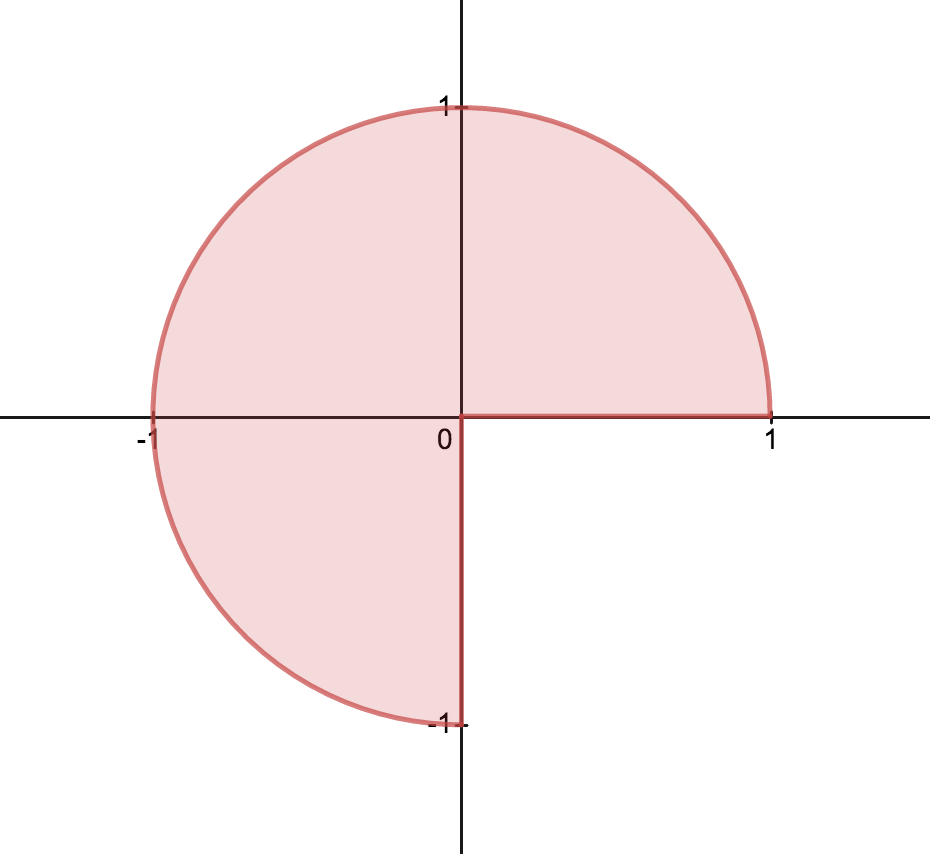
\includegraphics[width = 0.5\textwidth]{1.png}
        \caption{$K$. Plotted in \cite{Desmos}.}
        \label{fig:fig1}
    \end{figure}
    Note that $K$ is closed and bounded, and so is compact by Heine-Borel. Then 
    \begin{align*}
        f \paren{ \mathbf{x} } & = d \paren{ \mathbf{x} , K } \\
        & = \inf\limits_{ \mathbf{z} \in K } \norm{ \mathbf{x} - \mathbf{z} } \\
        & = \min\limits_{ \mathbf{z} \in K } \norm{ \mathbf{x} - \mathbf{z} }.
    \end{align*}
    Clearly for $\mathbf{x} \in K$, $f \paren{ \mathbf{x} } = 0$. Now, for $\mathbf{x} = (x,y) \notin K$ there are two cases to consider. 
    \begin{enumerate}
        \item If $x \leq 0$ or $y \geq 0$, then $\sqrt{x^2+y^2} > 1$ and $f \paren{ \mathbf{x} } = f(x,y)$ is just the length of the line segment connecting the point $(x,y)$ to $\frac{\mathbf{x}}{\norm{\mathbf{x}}} = \frac{(x,y)}{\sqrt{x^2,y^2}}$, which is 
        \begin{align*}
            \norm{ (x,y) - \frac{(x,y)}{\sqrt{x^2,y^2}} } & = \norm{ \paren{ 1 - \frac{1}{\sqrt{x^2+y^2}} } (x,y) } \\
            & = \abs{ 1 - \frac{1}{\sqrt{x^2+y^2}} } \norm{ (x,y) } \\
            & = \paren{ 1 - \frac{1}{\sqrt{x^2+y^2}} } \sqrt{x^2+y^2} && \text{since $\sqrt{x^2+y^2} > 1$} \\
            & = \sqrt{x^2+y^2} - 1.
        \end{align*}
        \begin{figure}[H]
            \centering
            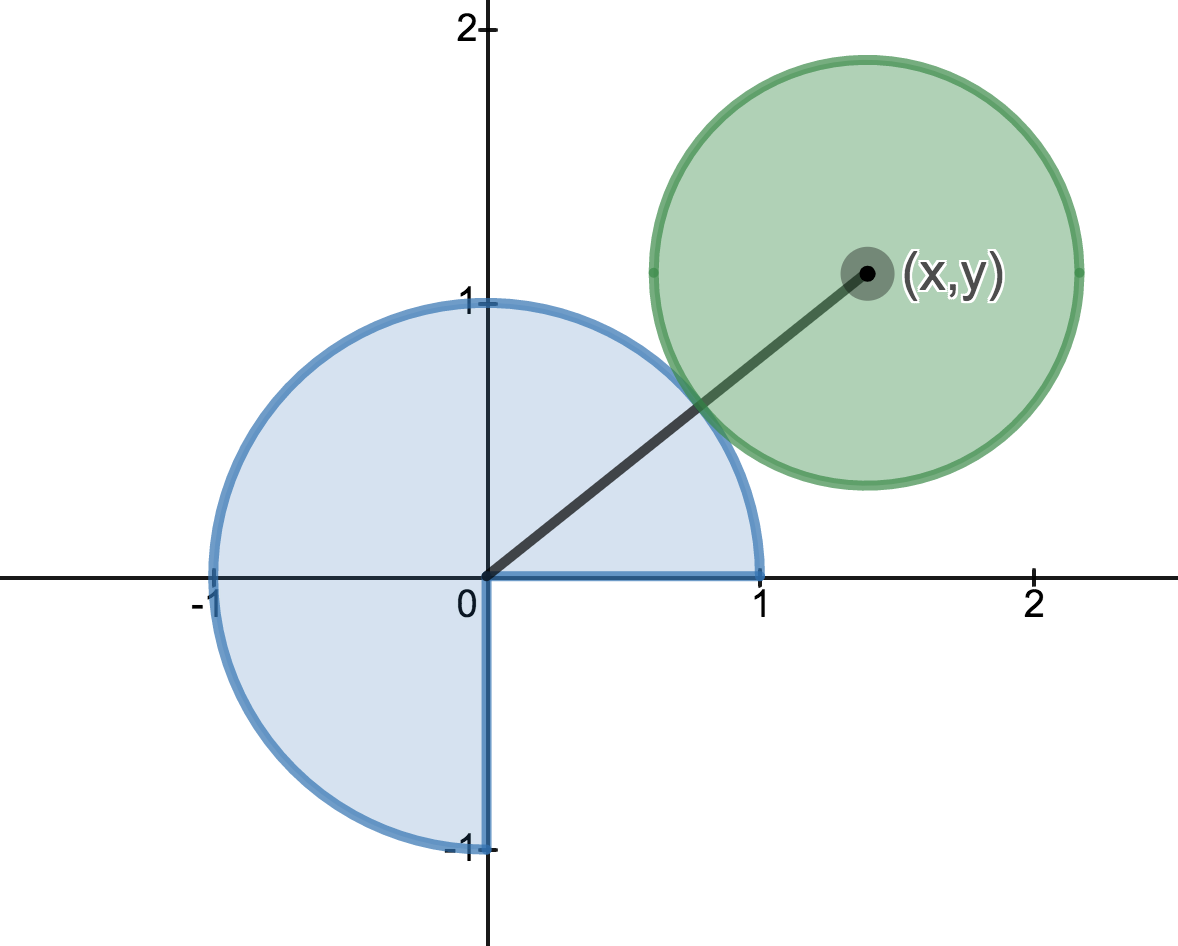
\includegraphics[width = 0.5\textwidth]{2.png}
            \caption{Diagram illustrating $f(x,y)$ for $x \leq 0$ or $y \geq 0$ and $\sqrt{x^2+y^2} > 1$. Plotted in \cite{Desmos}.}
            \label{fig:fig2}
        \end{figure}
        \item Now if $(x,y) \notin K$ and $x > 0$ and $y < 0$, there are two more cases to consider.
        \begin{enumerate}
            \item $\max\setb{x,|y|} \leq 1$. Then $f(x,y)$ is the length of the shortest line segment to either the $x$- or $y$-axes, so $f(x,y) = \min \setb{x,|y|}$.
            \begin{figure}[H]
                \centering
                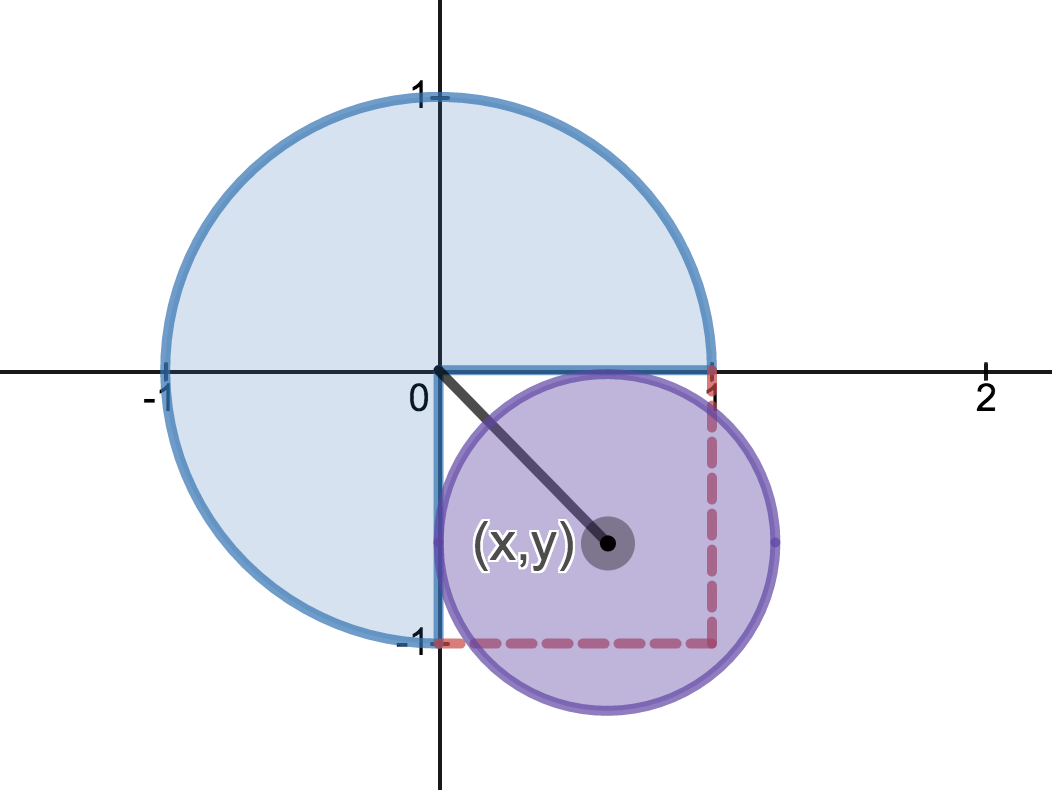
\includegraphics[width = 0.5\textwidth]{3.png}
                \caption{Diagram illustrating $f(x,y)$ for $x > 0$, $y < 0$, and $\max\setb{x,|y|} \leq 1$. Plotted in \cite{Desmos}.}
                \label{fig:fig3}
            \end{figure}
            \item $\max\setb{x,|y|} > 1$. This breaks down into three more cases.
            \begin{enumerate}
                \item $x > |y|$. Then $f(x,y)$ is the length of the line segment connecting $(x,y)$ to $(1,0)$, so 
                \[
                    f(x,y) = \norm{ (x,y) - (1,0) } = \sqrt{(x-1)^2+y^2}.
                \]
                \item $x < |y|$. Then $f(x,y)$ is the length of the line segment connecting $(x,y)$ to $(0,-1)$, so 
                \[
                    f(x,y) = \norm{ (x,y) - (0,-1) } = \sqrt{x^2+(y+1)^2}.
                \]
                \item $x = |y|$. Then $(x,y)$ is equidistant to $(1,0)$ and $(0,-1)$, so both of the above formulae apply. Writing $(x,y) = (x,-x)$, we check that they are consistent:
                \begin{align*}
                    (x-1)^2 + (-x)^2 & = (x-1)^2 + x^2 \\
                    x^2 + (-x+1)^2 & = x^2 + (x-1)^2 \checkmark.
                \end{align*}
            \end{enumerate}
             \begin{figure}[h]

                \begin{subfigure}{0.5\textwidth}
                    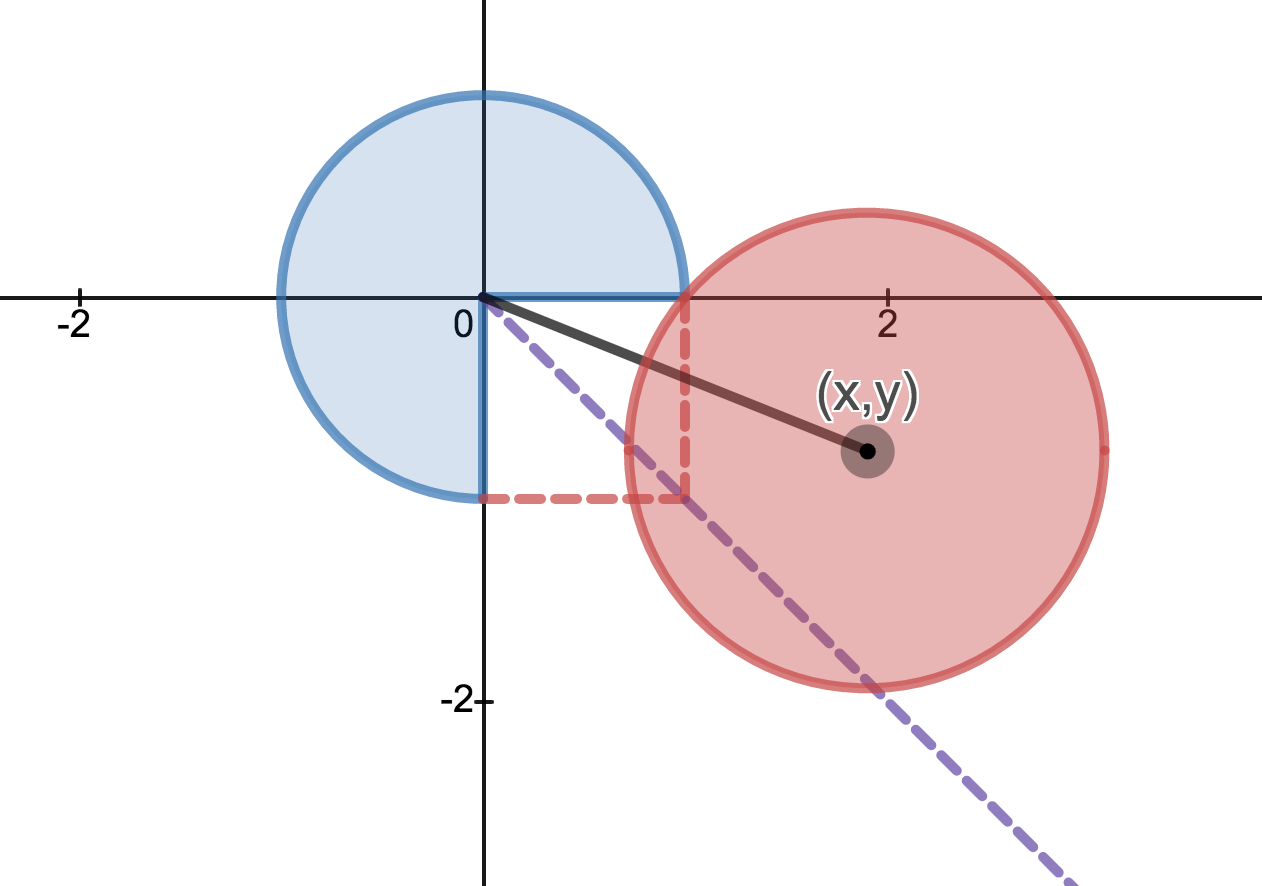
\includegraphics[width=\textwidth]{4} 
                    \caption{}
                    \label{fig:fig4}
                \end{subfigure}
                \begin{subfigure}{0.5\textwidth}
                    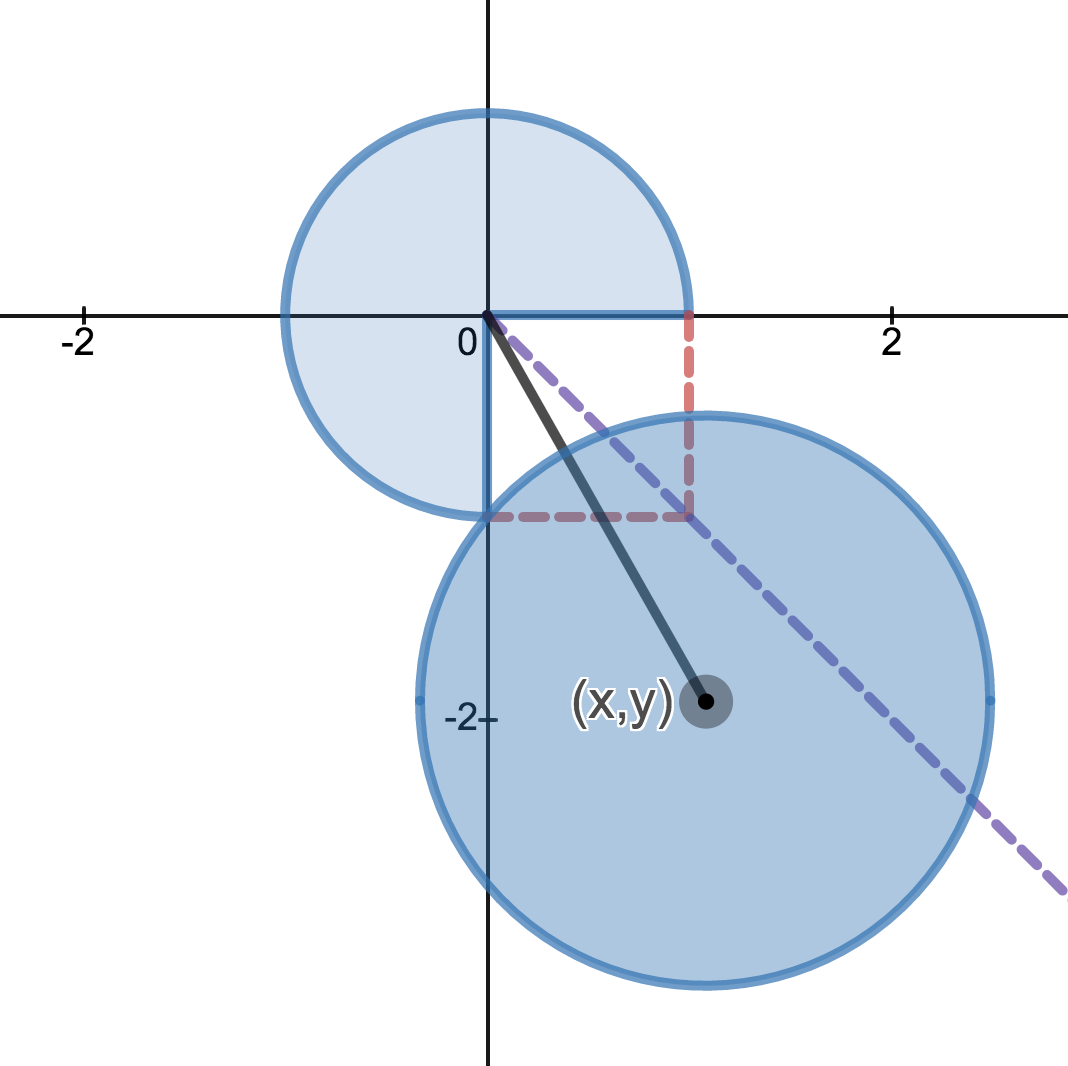
\includegraphics[width=\textwidth]{5}
                    \caption{}
                    \label{fig:fig5}
                \end{subfigure}

                \caption{Diagram illustrating $f(x,y)$ for $x > 0$, $y < 0$, and $\max\setb{x,|y|} < 1$. Plotted in \cite{Desmos}.}
                \label{fig:fig4and5}
            \end{figure}
        \end{enumerate}
    \end{enumerate}
    Finally, we can write down a closed form expression for $f$:
    \[
        f(x,y) = 
        \begin{cases}
            0 , & \quad x \leq 0 \text{ or } y \geq 0 , x^2 + y^2 \leq 1, \\
            \sqrt{x^2+y^2} - 1 , & \quad x \leq 0 \text{ or } y \geq 0 , x^2 + y^2 > 1 , \\
            \min\setb{x,|y|} , & \quad x > 0 , y < 0 , \max\setb{x,|y|} \leq 1 \\
            \sqrt{(x-1)^2+y^2} , & \quad x > 0 , y < 0 , \max\setb{x,|y|} > 1 , x \geq |y| , \\
            \sqrt{x^2+(y+1)^2} , & \quad x > 0 , y < 0 , \max\setb{x,|y|} > 1 , x < |y| .
        \end{cases}
    \]
    \begin{enumerate}[a)]
        \item Let $\eps > 0$, $\mathbf{x} , \mathbf{y} \in \real^2$, and without loss of generality take $f \paren{ \mathbf{x} } \geq f \paren{ \mathbf{y} }$. Then
        \begin{align*}
            \abs{ f \paren{ \mathbf{x} } - f \paren{ \mathbf{y} } } & = f \paren{ \mathbf{x} } - f \paren{ \mathbf{y} } = \min\limits_{ \mathbf{z} \in K } \norm{ \mathbf{x} - \mathbf{z} } - \min\limits_{ \mathbf{w} \in K } \norm{ \mathbf{y} - \mathbf{w} } \\
            & \leq \min\limits_{ \mathbf{z} \in K } \paren{  \norm{ \mathbf{x} - \mathbf{y} } + \norm{ \mathbf{y} - \mathbf{z} } } - \min\limits_{ \mathbf{w} \in K } \norm{ \mathbf{y} - \mathbf{w} } \\ 
            & = \norm{ \mathbf{x} - \mathbf{y} } + \min\limits_{ \mathbf{z} \in K } \norm{ \mathbf{y} - \mathbf{z} } - \min\limits_{ \mathbf{w} \in K } \norm{ \mathbf{y} - \mathbf{w} } \\
            & = \norm{ \mathbf{x} - \mathbf{y} } + \min\limits_{ \mathbf{w} \in K } \norm{ \mathbf{y} - \mathbf{w} } - \min\limits_{ \mathbf{w} \in K } \norm{ \mathbf{y} - \mathbf{w} } = \norm{ \mathbf{x} - \mathbf{y} } \\
            & < \eps
        \end{align*}
        for $\norm{ \mathbf{x} - \mathbf{y} } < \eps$. Therefore $f$ is uniformly continuous.
        \item $f$ is not differentiable on 
        \[
            \setb{ (x,y) \, \middle| \, \max \setb{x,y} \leq 1 , x > 0 , y < 0 },
        \]
        due to the minimum function itself not being differentiable. 
    \end{enumerate}
\end{proof}
\subsection{Problem 4}
\begin{enumerate}
    \item Give an example of a bounded function 
    \[
        h_1 : [0,1] \to \real
    \]
    such that $h_1$ has infinitely many discontinuities but is Riemann integrable.
    \item Give an example of a bounded function 
    \[
        h_2 : [0,1] \to \real
    \]
    such that $h_2$ is not Riemann integrable.
\end{enumerate}
\begin{proof}[Answer]
    \noindent 
    \begin{enumerate}[a)]
        \item Recall that a bounded function $f : [a,b] \to \real$ is Riemann-integrable on $[a,b]$ if the set of discontinuities of $f$ has measure zero. Let $h_1 :[0,1] \to \real$ be given by 
        \[
            h_1(x) \coloneqq 
            \begin{cases}
                1 , & \quad x = \frac{1}{n} \text{ for some } n \in \z^+ , \\
                0 , & \quad \text{otherwise}.
            \end{cases}
        \]
        Then $h_1$ is discontinuous at each $x_n = \frac{1}{n}$ for $n \in \z^+$, and so $h_1$ has infinitely many discontinuities. However, $h_1$ has only countably many discontinuities, so $f$ is Riemann integrable, and in fact 
        \[
            \int_0^1 h_1(x) \, \mathrm{d}x = 0.
        \]
        \item Let $h_2 : [0,1] \to \real$ be given by 
        \[
            h_2(x) \coloneqq 
            \begin{cases}
                1 , & \quad x \in \q, \\
                0 , & \quad x \notin \q.
            \end{cases}
        \]
        Clearly $h_2$ is bounded. Let 
        \[
            \mathcal{P} \coloneqq \setb{ 0 = x_0 < x_1 < x_2 < \dotsb < x_{n-1} < x_n = 1 }
        \]
        be a partition of $[0,1]$. Then as there are infinitely many rationals and irrationals in each $\sqbrack{ x_{i-1} , x_i }$, $M_i = 1$ and $m_i = 0$ for all $1 \leq i \leq n$. Thus
        \begin{align*}
            U(h_2,\mathcal{P}) & = \sum\limits_{i = 1}^n M_i \Delta x_i = \sum\limits_{i = 1}^n \Delta x_i = 1, \\
            L(h_2,\mathcal{P}) & = \sum\limits_{i = 1}^n m_i \Delta x_i = 0.
        \end{align*}
        Thus 
        \begin{align*}
            \overline{\int_0^1} h_2(x) \mathrm{d}x & = \inf\limits_{\mathcal{P} \in \mathscr{P}[0,1]} U(h_2,P) = 1, \\
            \underline{\int_0^1} h_2(x) \mathrm{d}x & = \sup\limits_{\mathcal{P} \in \mathscr{P}[0,1]} U(h_2,P) = 0,
        \end{align*}
        and so $h_2$ is not Riemann-integrable.
    \end{enumerate}
\end{proof}
\subsection{Problem 5}
Prove that there is no function
\[
    f : \setb{ (x,y) \in \real^2 \, \middle| \, x^2 + y^2 = 1 } \to \real
\]
which is continuous and one to one.
\begin{proof}[Answer]
    By way of contradiction, suppose that there exists $f : S^1 = \setb{ (x,y) \in \real^2 \, \middle| \, x^2 + y^2 = 1 } \to \real$ continuous and injective. Since $S^1$ is compact and connected, $f(S^1)$ is also compact and connected in $\real$, and so it is equal to a closed interval $[a,b]$ for some $a \leq b$. Since $S^1$ is (uncountably) infinite and $f$ is injective, $a < b$. Let $a < c < b$, then by injectivity of $f$ there exists a unique $p \in S^1$ such that $f(p) = c$. Then the restriction of $f$ to $S^1 \setminus \setb{ p }$ is still a continuous injection, and its image is precisely 
    \[
        f \paren{ S^1 } \setminus \setb{ f(p) } = [a,b] \setminus \setb{ c } = [a,c) \cup (c,b].
    \]
    However, $S^1 \setminus \setb{ p }$ is connected while $[a,c) \cup (c,b]$ is not, contradicting the continuity of $f$. Therefore no such function $f$ exists.
    
    In particular, this shows that $S^1$ is not homeomorphic to $\real$ or to a closed interval $[a,b]$.
\end{proof}
\subsection{Problem 6}
Prove that every uncountable subset of $\real^n$ has an accumulation point.
\begin{proof}[Answer]
    We prove the contrapositive: if $A \subseteq \real^n$ has no accumulation points, then it must be countable. Since $A$ has no accumulation points, for each $a \in A$ there exists an open neighborhood $a \in U_a \subset \real^n$ such that $U_a \cap A = \setb{ a }$. Then the collection $\setb{ U_a }_{a \in A}$ is an open cover of $A$. Since $\real^n$ is metrizable and second-countable, so is $A$, and in particular $A$ is Lindel\"of. Thus there exists a countable subcover $\setb{ U_{a_n} }_{n = 1}^{\infty}$. Since each $U_{a_n}$ intersects $A$ in exactly one element of $A$, this shows that $A$ has at most countably infinitely many elements. 
\end{proof}
\subsection{Problem 7 \texorpdfstring{\cite{Lin}}{}}
Prove that for $k \in \n$ large enough, the system of equations
\begin{align*}
    x + x^{10} y^5 \sin \paren{ xy } & = 10^{-k} \\
    x + y - \paren{ x^2 + y^2 }^3 e^{xy} & = \frac{1}{k}
\end{align*}
has a solution $\paren{ x_k , y_k }$.
\begin{proof}[Answer]
    Let $f : \real^2 \to \real^2$ be given by 
    \[
        f(x,y) \coloneqq 
        \begin{bmatrix}
            x + x^{10} y^5 \sin \paren{ xy } \\
            x + y - \paren{ x^2 + y^2 }^3 e^{xy}
        \end{bmatrix}.
    \]
    Then $Df$ is given by 
    \begin{align*}
        (Df)(x,y) & = 
        \begin{bmatrix}
            1 + 10x^9y^5\sin(xy) + x^{10}y^6\cos(xy) & 5x^{10}y^4\sin(xy) + x^{11}y^5\cos(xy) \\
            1 - 6x\paren{x^2+y^2}^2e^{xy} - y\paren{x^2+y^2}^3e^{xy} & 1 - 6y\paren{x^2+y^2}^2e^{xy} - x\paren{x^2+y^2}^3e^{xy}
        \end{bmatrix} \\
        & = 
        \begin{bmatrix}
            1 + x^9 y^5 \sqbrack{ 10 \sin(xy) + xy \cos(xy) } & x^{10} y^4 \sqbrack{ 5 \sin(xy) + xy \cos(xy) } \\
            1 - \paren{ x^2 + y^2 }^2 \paren{ x^2y + 6x + y^3 } e^{xy} & 1 - \paren{ x^2 + y^2 }^2 \paren{ x^3 + xy^2 + 6y } e^{xy}
        \end{bmatrix}
    \end{align*}
    At $(x,y) = (0,0)$,
    \[
        (Df)(0,0) = 
        \begin{bmatrix}
            1 & 0 \\
            1 & 1
        \end{bmatrix}
    \]
    and 
    \[
        \det \paren{ (Df)(0,0) } = 1 - 0 = 1 \neq 0.
    \]
    By Inverse Function Theorem, there exists open neighborhoods $U , V \subseteq \real^2$ of $(0,0)$ such that $f : U \to V$ has a continuously differentiable inverse $g : V \to U$. Let $\eps > 0$ such that $B_{\eps}(0) \subseteq V$, then choose $k \in \z^+$ large enough such that $k > \frac{\sqrt{2}}{\eps}$. Then $\paren{ 10^{-k} , \frac{1}{k} } \in B_{\eps}(0)$, since \begin{align*}
        \norm{ \paren{ 10^{-k} , \frac{1}{k} } } & = 10^{-2k} + \frac{1}{k^2} < \frac{1}{k^2} + \frac{1}{k^2} \\
        & = \frac{2}{k^2} < 2\frac{\eps}{2} \\
        & = \eps.
    \end{align*}
    Thus there exists a unique $\paren{ x_k , y_k } \in U$ such that $f \paren{ x_k , y_k } = \paren{ 10^{-k} , \frac{1}{k} }$.
\end{proof}
\subsection{Problem 8 \texorpdfstring{\cite{Leon}}{}}
In each case, give an example of a sequence of continuous and bounded functions $f_n : \real \to \real$ such that
\begin{enumerate}[a)]
    \item for each $x \in \real$, $f_n(x) \to f(x)$ but $f_n$ does not converge to $f$ uniformly in $\real$.
    \item $f_n \to f$ uniformly in $\real$ but
    \[
        \lim\limits_{n \to \infty} \int_{-\infty}^{\infty} f_n \neq \int_{-\infty}^{\infty} f.
    \]
    \item $f_n$ does not converge uniformly to $f$ but 
    \[
        \lim\limits_{n \to \infty} \int_{-\infty}^{\infty} f_n = \int_{-\infty}^{\infty} f.
    \]
    \end{enumerate}
\begin{proof}[Answer]
    \noindent 
    \begin{enumerate}[a)]
        \item For each $n \in \z^+$, let 
        \[
            f_n(x) \coloneqq 
            \begin{cases}
                1 - |x|^n , & \quad -1 \leq x \leq 1 , \\
                0 , & \quad \text{otherwise}.
            \end{cases}
        \]
        On $[-1,1]$ and $\real \setminus [-1,1]$, $f_n$ is continuous, and since
        \[
            \lim\limits_{x \to \pm 1} f_n(x) = f_n(\pm1) = 0,
        \]
        $f_n$ is continuous for all $x \in \real$.
        Then $f_n$ converges to $f = \chi_{(-1,1)}$, since $f_n(\pm1) = 0$ for all $n \in \z^+$, while for all $-1 < x < 1$, 
        \begin{align*}
            \lim\limits_{n \to \infty} f_n(x) & = \lim\limits_{n \to \infty} 1 - |x|^n = 1 - 0 = 1.
        \end{align*}
        However, this convergence is not uniform, since $f$ is not continuous (uniform limit of continuous functions is continuous).
        \item Let
        \[
            g(x) \coloneqq \frac{1}{x^2+1},
        \]
        and let $f_n(x) \coloneqq \frac{1}{n} g \paren{  \frac{x}{n} }$ for each $n \in \z^+$. Then $f_n$ converges uniformly to $f = 0$, since
        \begin{align*}
            \sup\limits_{x \in \real} \abs{ f_n(x) - f(x) } & = \sup\limits_{x \in \real} \abs{ \frac{1}{n} \frac{1}{\paren{ \frac{x}{n} }^2+1} }  = \sup\limits_{x \in \real} \frac{1}{\frac{x^2}{n}+n} \\
            & = \frac{1}{n} \to 0
        \end{align*}
        as $n \to \infty$. However,
        \begin{align*}
            \int_{-\infty}^{\infty} f_n(x) \, \mathrm{d}x & = \int_{-\infty}^{\infty} \frac{1}{n} g \paren{  \frac{x}{n} } \, \mathrm{d}x = \int_{-\infty}^{\infty} g(y) \, \mathrm{d}y \\
            & = \int_{-\infty}^{\infty} \frac{\mathrm{d}y}{y^2+1} = \pi
        \end{align*}
        for all $n \in \z^+$, and so 
        \[
            \lim\limits_{n \to \infty} \int_{-\infty}^{\infty} f_n(x) \, \mathrm{d}x \neq \int_{-\infty}^{\infty} f(x) \, \mathrm{d}x.
        \]
        \item Using the same functions from part a), we have 
        \begin{align*}
            \int_{-\infty}^{\infty} f_n(x) \, \mathrm{d}x & = \int_{-1}^1 \paren{ 1 - |x|^n } \, \mathrm{d}x = 2 \int_0^1 \paren{ 1 - |x|^n } \, \mathrm{d}x \\
            & = 2 \int_0^1 \paren{ 1 - x^n } \, \mathrm{d}x = 2 \paren{ \left. x - \frac{x^{n+1}}{n+1} \right|_{0}^{1} } \\
            & = 2 \paren{ 1 - \frac{1}{n+1} - 0 } = 2 \paren{ 1 - \frac{1}{n+1} },
        \end{align*}
        and so 
        \begin{align*}
            \lim\limits_{n \to \infty} \int_{-\infty}^{\infty} f_n(x) \, \mathrm{d}x & = \lim\limits_{n \to \infty} 2 \paren{ 1 - \frac{1}{n+1} } = 2 ( 1 - 0 ) = 2.
        \end{align*}
        Lastly,
        \begin{align*}
            \int_{-\infty}^{\infty} f(x) \, \mathrm{d}x & = \int_{-1}^{1} \, \mathrm{d}x = 1 - (-1) = 2,
        \end{align*}
        and so 
        \[
            \lim\limits_{n \to \infty} \int_{-\infty}^{\infty} f_n(x) \, \mathrm{d}x = \int_{-\infty}^{\infty} f(x) \, \mathrm{d}x.
        \]
    \end{enumerate}
\end{proof}
\newpage
\section{Spring 2014 [Completed]}
Solve 3 of the 4 problems in both Parts 1 and 2. Each problem is worth 10 points. This exam will test the extent of your knowledge and the clarity of your mathematical writing, so be sure to show all your working and justify all your steps. You must pass \textbf{both} parts in order to pass the exam. 
\subsection{Problem 1 \texorpdfstring{\cite{Cesaro}}{}}
\begin{enumerate}[(a)]
    \item Let $\setb{ s_n }_{n = 1}^{\infty}$ be a sequence of real numbers. Define the sequence 
    \[
        \sigma_n = \frac{1}{n} \sum\limits_{k = 1}^n s_k.
    \]
    Prove that if $\lim_{n \to \infty} s_n = L$, then $\lim_{n \to \infty} \sigma_n = L$.
    \item Give an example that shows the converse is false.
\end{enumerate}
\begin{proof}[Answer]
    \noindent
    \begin{enumerate}[(a)]
        \item We show that 
        \[
            \liminf\limits_{n \to \infty} s_n \leq \liminf\limits_{n \to \infty} \sigma_n \leq \limsup\limits_{n \to \infty} \sigma_n \leq \limsup\limits_{n \to \infty} s_n .
        \]
        Then if $\setb{ s_n }_{n = 1}^{\infty}$ converges, so does $\setb{ \sigma_n }_{n = 1}^{\infty}$, and they both converge to the same limit.
        
        By definition of the limit superior and limit inferior, we have
        \begin{align*}
            \liminf\limits_{n \to \infty} s_n & \leq \limsup\limits_{n \to \infty} s_n , \\
            \liminf\limits_{n \to \infty} \sigma_n & \leq \limsup\limits_{n \to \infty} \sigma_n .
        \end{align*}
        Now, recall that for any sequence $\setb{ s_n }_{n = 1}^{\infty}$,
        \[
            \limsup\limits_{n \to \infty} s_n = \lim\limits_{n \to \infty} \paren{ \sup\limits_{m \geq n} s_m }.
        \]
        Fix $k \leq m$, then 
        \begin{align*}
            \sigma_m & = \frac{1}{m} \sum\limits_{j = 1}^m s_j = \frac{1}{m} \paren{ \sum\limits_{j = 1}^k s_j + \sum\limits_{j = k + 1}^m s_j } \\
            & = \frac{1}{m} \sum\limits_{j = 1}^k s_j + \frac{1}{m} \sum\limits_{j = k + 1}^m s_j \leq \frac{1}{m} \sum\limits_{j = 1}^k s_j + \frac{m - (k+1) - 1}{m} \paren{ \sup\limits_{\ell \geq k + 1} s_{\ell} } \\
            & = \frac{1}{m} \sum\limits_{j = 1}^k s_j + \frac{m - k}{m} \paren{ \sup\limits_{\ell \geq k} s_{\ell} }.
        \end{align*}
        Thus 
        \begin{align*}
            \sup\limits_{m \geq n} \sigma_m & \leq \sup\limits_{m \geq n} \sqbrack{ \frac{1}{m} \sum\limits_{j = 1}^k s_j + \frac{m - k}{m} \paren{ \sup\limits_{\ell \geq k} s_{\ell} } } \\
            & \leq \sup\limits_{m \geq n} \paren{ \frac{1}{m} \sum\limits_{j = 1}^k s_j } + \sup\limits_{m \geq n} \sqbrack{ \frac{m - k}{m} \paren{ \sup\limits_{\ell \geq k} s_{\ell} } } \\
            & = \frac{1}{n} \sum\limits_{j = 1}^k s_j + \paren{ 1 - \frac{k}{n} } \paren{ \sup\limits_{\ell \geq k} s_{\ell} },
        \end{align*}
        and so 
        \begin{align*}
            \lim\limits_{n \to \infty} \paren{ \sup\limits_{m \geq n} \sigma_m } & \leq \lim\limits_{n \to \infty} \sqbrack{ \frac{1}{n} \sum\limits_{j = 1}^k s_j + \paren{ 1 - \frac{k}{n} } \paren{ \sup\limits_{\ell \geq k} s_{\ell} } } \\
            & = \lim\limits_{n \to \infty} \paren{ \frac{1}{n} \sum\limits_{j = 1}^k s_j } + \lim\limits_{n \to \infty} \sqbrack{ \paren{ 1 - \frac{k}{n} } \paren{ \sup\limits_{\ell \geq k} s_{\ell} } } \\
            & = 0 + \sup\limits_{\ell \geq k} s_{\ell}.
        \end{align*}
        Finally, 
        \begin{align*}
            \lim\limits_{k \to \infty} \sqbrack{ \lim\limits_{n \to \infty} \paren{ \sup\limits_{m \geq n} \sigma_m } } & \leq \lim\limits_{k \to \infty} \paren{ \sup\limits_{\ell \geq k} s_{\ell} } , \\
            \limsup\limits_{n \to \infty} \sigma_n & \leq \lim\limits_{n \to \infty} \paren{ \sup\limits_{m \geq n} s_{m} } \\
            & = \limsup\limits_{n \to \infty} s_n.
        \end{align*}
        A similar argument shows that 
        \[
            \liminf\limits_{n \to \infty} s_n \leq \liminf\limits_{n \to \infty} \sigma_n.
        \]
        \item Let 
        \[
            s_n \coloneqq 
            \begin{cases}
                1 , & \quad n \text{ even, } \\
                0 , & \quad n \text{ odd. }
            \end{cases}
        \]
        Then $\limsup\limits_{n \to \infty} s_n = 1$ while $\liminf\limits_{n \to \infty} s_n = 0$, so $\setb{ s_n }_{n=1}^{\infty}$ does not converge. However, for $n$ even,
        \begin{align*}
            \sigma_n & = \frac{1}{n} \big( \underbrace{ 1 + 1 + \dotsb + 1 }_{ \text{$n/2$ times} } \big) = \frac{n/2}{n} = \frac{1}{2},
        \end{align*}
        while for $n$ odd,
        \begin{align*}
            \sigma_n & = \frac{1}{n} \big( \underbrace{ 1 + 1 + \dotsb + 1 }_{ \text{$n/2$ times} }  + 0 \big) = \frac{n/2}{n} = \frac{1}{2}.
        \end{align*}
        Thus $\sigma_n = \frac{1}{2}$ for all $n \in \z^+$, and so $\lim\limits_{n \to \infty} \sigma_n = \frac{1}{2}$.
    \end{enumerate}
\end{proof}
\subsection{Problem 2 \texorpdfstring{\cite{Nguyen}}{}}
Let $A \subset \real^2$ be nonempty. Define the distance of a point $x \in \real^2$ to $A$ by 
\[
    d(x) = \inf \setb{ \norm{ x - y } : y \in A },
\]
where $\norm{x}$ denotes the Euclidean norm of a vector in $\real^2$.
\begin{enumerate}[(a)]
    \item Prove that 
    \[
        \abs{ d \paren{ x_1 } - d \paren{ x_2 } } \leq \norm{ x_1 - x_2 },
    \]
    for every $x_1 , x_2 \in \real^2$.
    \item Prove that $d : \real^2 \to \real$ is continuous.
    \item Give an example illustrating that $d$ may not be differentiable at some point $x \in \real^2$.
\end{enumerate}
\begin{proof}[Answer]
    See Spring 1994, Problem 3. For part (c), take $A \coloneqq \setb{ (0,0) }$. Then $d(x,y) = \abs{ x }$ is not differentiable at $(0,0)$, and in fact at any $(0,y)$ for $y \in \real$.
\end{proof}
\subsection{Problem 3}
Define 
\[
    P(x,y,z) = x^3 + 2xy^2 - 7z^3 + 3y + 1.
\]
\begin{enumerate}[(a)]
    \item Prove that there exists a function $z = f(x,y)$ such that 
    \begin{itemize}
        \item $f(x,y)$ is $C^1$ in a neighborhood $N$ of $(x,y) = (1,1)$,
        \item $P(x,y,f(x,y)) = 0$ for $(x,y) \in N$,
        \item $f(1,1) = 1$.
    \end{itemize}
    \item Find the tangent plane at the point $(1,1,1)$ on the surface defined by the graph $z = f(x,y)$, $(x,y) \in N$.
\end{enumerate}
\begin{proof}[Answer]
    \noindent
    \begin{enumerate}[(a)]
        \item Note that
        \begin{align*}
            P(1,1,1) & = 1^3 + 3 \cdot 1 \cdot 1^2 - 7 \cdot 1^3 + 3 \cdot 1 + 1 \\
            & = 1 + 2 - 7 + 3 + 1 \\
            & = 0.
        \end{align*}
        Then
        \begin{align*}
            P_x(x,y,z) & = 3x^2 + 2y^2, \\
            P_x(1,1,1) & = 3 \cdot 1^2 + 2 \cdot 1^2 = 3 + 2 = 5 \neq 0, \\
            P_y(x,y,z) & = 4y + 3, \\
            P_y(1,1,1) & = 4\cdot1 + 3 = 4 + 3 = 7 \neq 0, \\
            P_z(x,y,z) & = -21z^2, \\
            P_z(1,1,1) & = -21\cdot1^2 = -21.
        \end{align*}
        By Implicit Function Theorem, there exists an open neighborhood $N$ of $(1,1) \in \setb{ (x,y,0) \in \real^2 \, \middle| \, x,y \in \real}$ and an open neighborhood $U$ of $(1,1,1) \in \real^3$ such that $\inv{P} \paren{ \setb{ 0 } } \cap U$ is the graph of a $C^1$ function $f : N \to U$. Thus $P(x,y,f(x,y)) = 0$ for all $(x,y) \in N$ and $f(1,1) = 1$. 
        \item The tangent plane to the point $(1,1,1)$ on the surface $f(N)$ is given by 
        \begin{align*}
            \nabla P(1,1,1) \cdot (x-1,y-1,z-1) & = (5,7,-21) \cdot (x-1,y-1,z-1) \\
            & = 5x - 5 + 7y - 7 -21z + 21 \\
            & = 5x + 7y - 21z + 9 = 0.
        \end{align*}
    \end{enumerate}
\end{proof}
\subsection{Problem 4}
\begin{enumerate}[(a)]
    \item Given a set $A \subset \real^n$, define its closure, $\mathrm{cl} A$.
    \item Given a set $A \subset \real^n$, define its interior, $\mathrm{int} A$.
    \item Using your definition of closure above, prove or disprove the following statement: $\mathrm{cl}(A \cup B) = \mathrm{cl}A \cup \mathrm{cl}B$, for every $A , B \subset \real^n$.
    \item Using your definition of closure above, prove or disprove the following statement: $\mathrm{int}(A \cup B) = \mathrm{int}A \cup \mathrm{int}B$, for every $A , B \subset \real^n$.
\end{enumerate}
\begin{proof}[Answer] 
    \noindent
    \begin{enumerate}[(a)]
        \item 
        \[
            \overline{A} = \bigcap\limits_{ \substack{
                A \subseteq C \\
                C \text{ closed}
            } } C.
        \]
        Note that $\overline{A}$ is itself closed.
        \item 
        \[
            A^{\mathrm{o}} = \bigcup\limits_{ \substack{
                U \subseteq A \\
                U \text{ open}
            } } U.
        \]
        Note that $\interior{A}$ is itself open, and that 
        \[
            \interior{A} \subseteq A \subseteq \overline{A}.
        \]
        \item Since $\overline{A}$ and $\overline{B}$ are closed, $\overline{A} \cup \overline{B}$ is a closed set that contains $A \cup B$, and so $\overline{A \cup B} \subseteq \overline{A} \cup \overline{B}$. Conversely, since $\overline{A \cup B}$ is a closed set that contains $A$ and $B$, $\overline{A}$ and $\overline{B}$ are both contained in $\overline{A \cup B}$, so $\overline{A} \cup \overline{B} \subseteq \overline{A \cup B}$.
        \item Since $\interior{A}$ and $\interior{B}$ are open, $\interior{A} \cup \interior{B}$ is an open set contained in $A \cup B$, and so $\interior{A} \cup \interior{B} \subseteq \interior{ \paren{ A \cup B } }$. 
        
        However, this inclusion can be strict: in $\real$, let $A \coloneqq \q$, $B \coloneqq \real \setminus \q$. Since every open interval contains both rational and irrational numbers, $\interior{A} = \interior{B} = \varnothing$, however $\interior{ \paren{ A \cup B } } = \interior{\real} = \real$.
    \end{enumerate}
\end{proof}
\newpage
\section{Fall 2014 [Answered]}
Do \textbf{only} 3 problems from each part of the exam. Start each problem on a new sheet of paper. Write on one side only and avoid the edges since the exams will be copied for grading. Each problem is worth 10 points; when problems have parts, the parts are equally weighted unless the explicit is indicated.

\textbf{Be sure to justify all of your answers by citing theorems or showing computations. Details matter; the right idea or even the right answer will not get full credit without clear justification.}
\subsection{Problem 1}
Find a real number $c$ such that 
\[
    \abs{ c - \int_{-.2}^{.7} \frac{1 - \cos x}{x} } < .001
\]
\begin{proof}[Answer]
    UNANSWERED
\end{proof}
\subsection{Problem 2}
Prove or disprove: If $f : \real \to \real$ is a differentiable function such that $f(x) > x^2 \forall x \in \real$, then $\sup \abs{ f'(x) } = +\infty$.
\begin{proof}[Answer]
    Let $x > 0$, then $f$ satisfies the Mean Value Theorem on $[0,x]$, so there exists $0 < y < x$ such that 
    \[
        f'(y) = \frac{f(x) - f(0)}{x - 0}.
    \]
    Then 
    \begin{align*}
        f'(y) & = \frac{f(0) - f(x)}{0 - x} > \frac{0^2 - f(x)}{-x} \\
        & = \frac{f(x)}{x} > \frac{x^2}{x} \\
        & = x.
    \end{align*}
    Thus for all $x > 0$, there exists $0 < y < x$ such that $f'(y) > x$. Therefore $\sup\limits_{y \in \real} \abs{ f'(y) } = +\infty$.
\end{proof}
\subsection{Problem 3 \texorpdfstring{\cite{Dennis}}{}}
Show that 
\[
    f(t) = \sum\limits_{n = 1}^{\infty} \frac{(-1)^n}{n} \cos(t/n)
\]
defines a continuously differentiable function on all real numbers.
\begin{proof}[Answer]
    Let $g : \real \to \real$ be given by 
    \[
        g(t) \coloneqq \sum\limits_{n = 1}^{\infty} \underbrace{ \frac{(-1)^{n-1}}{n^2} \sin \paren{ \frac{t}{n} } }_{ \eqqcolon g_n(t) }.
    \]
    We show that $g$ is continuous by showing that the series converges uniformly. Note that for all $t \in \real$,
    \begin{align*}
        \abs{ g_n(t) } & = \abs{ \frac{(-1)^{n-1}}{n^2} \sin \paren{ \frac{t}{n} } } = \frac{1}{n^2} \abs{ \sin \paren{ \frac{t}{n} } } \leq \frac{1}{n^2}.
    \end{align*}
    Since
    \[
        \sum\limits_{n = 1}^{\infty} \frac{1}{n^2} = \frac{\pi^2}{6} < \infty,
    \]
    the series converges uniformly by Weierstrass $M$ Test. Since $g_n$ is continuous for all $n \in \z^+$, $g$ is continuous, and so for all $t \in \real$,
    \begin{align*}
        \int_{\pi}^t g \paren{t'} \, \mathrm{d}t' & = \int_{0}^t \sqbrack{ \sum\limits_{n = 1}^{\infty} \frac{(-1)^{n-1}}{n^2} \sin \paren{ \frac{t'}{n} } } \, \mathrm{d}t' = \sum\limits_{n = 1}^{\infty} \frac{(-1)^{n-1}}{n^2} \int_{0}^{t} \sin \paren{ \frac{t'}{n} } \, \mathrm{d}t' \\
        & = \sum\limits_{n = 1}^{\infty} \frac{(-1)^{n-1}}{n^2} \sqbrack{ \left. -n \cos \paren{ \frac{t'}{n} } \right|_{t' = 0}^{t' = t} } = \sum\limits_{n = 1}^{\infty} \frac{(-1)^{n}}{n} \sqbrack{ \cos \paren{ \frac{t}{n} } - \cos (0) } \\
        & = \sum\limits_{n = 1}^{\infty} \frac{(-1)^{n}}{n} \sqbrack{ \cos \paren{ \frac{t}{n} } - 1 } = \sum\limits_{n = 1}^{\infty} \frac{(-1)^{n}}{n} \cos \paren{ \frac{t}{n} } - \sum\limits_{n = 1}^{\infty} \frac{(-1)^{n}}{n} \\
        & = f(t) + \log 2.
    \end{align*}
    Therefore $f$ is an antiderivative of a continuous function, and so is continuously differentiable. 
\end{proof}
\subsection{Problem 4}
Let $(X,d)$ be a metric space.
\begin{enumerate}[label={[\arabic*]}]
    \stepcounter{enumi}
    \stepcounter{enumi}
    \stepcounter{enumi}
    \item 
    \begin{enumerate}[(a)]
        \item Complete the following definitions.
        \begin{enumerate}[(i)]
            \item $(X,d)$ is compact if.....(Do not trivialize part (b) by choosing a definition that contains completeness. There are several other possibilities.)
            \item $(X,d)$ is complete if....
        \end{enumerate}
    \end{enumerate}
    \stepcounter{enumi}
    \item 
    \begin{enumerate}[(a)]
        \setcounter{enumi}{2}
        \item Using only the definitions that you gave of ''complete'' and ''compact'', show that compactness implies completeness.
    \end{enumerate}
\end{enumerate}
\begin{proof}[Answer]
    \noindent
    \begin{enumerate}[(a)]
        \item 
        \begin{enumerate}[(i)]
            \item $(X,d)$ is compact if sequence $\setb{ x_n }_{n = 1}^{\infty}$ has a convergent subsequence $\setb{ x_{n_k} }_{k = 1}^{\infty}$.
            \item $(X,d)$ is complete if every Cauchy sequence $\setb{ x_n }_{n = 1}^{\infty}$ converges.
        \end{enumerate}
        \item 
        \begin{lemma}
            Let $(X,d)$ be a metric space, and let $\setb{ x_n }_{n=1}^{\infty} \subseteq X$ be a Cauchy sequence. If $\setb{ x_n }_{n=1}^{\infty}$ has a convergent subsequence $\setb{ x_{n_k} }_{k=1}^{\infty}$ converging to, say, $x_0 \in X$, then $\setb{ x_n }_{n=1}^{\infty}$ also converges to $x_0$. 
        \end{lemma}
        \begin{proof}
            Let $\epsilon > 0$, then there exists $N_1 \in \z^+$ such that for all $n , m > N$,
            \[
                d(x_n,x_m) < \frac{\epsilon}{2}.
            \]
            Since $\setb{ x_{n_k} }_{k=1}^{\infty}$ converges to $x_0$, there exists $N_2 \in \z^+$ such that for all $k > N_2$, 
            \[
                d \paren{ x_{n_k} , x_0 } < \frac{\epsilon}{2}.
            \]
            Take $N \coloneqq \max \setb{N_1,N_2}$. Let $m_k$ be the index for the convergent subsequence, then for all $n , k , m_k > N$,
            \begin{align*}
                d(x_n,x_0) & \leq d \paren{ x_n , x_{m_k} } + d \paren{ x_{m_k} , x_0 } < \frac{\epsilon}{2} + \frac{\epsilon}{2} = \epsilon.
            \end{align*}
            Therefore $\setb{ x_n }_{n=1}^{\infty}$ converges to $x_0$.
        \end{proof}
        Suppose $(X,d)$ is a compact metric space. Let $\setb{ x_n }_{n = 1}^{\infty} \subseteq X$ be a Cauchy sequence. Then by compactness of $X$, $\setb{ x_n }_{n = 1}^{\infty}$ has a convergent subsequence $\setb{ x_{n_k} }_{k = 1}^{\infty}$, so by the above lemma $\setb{ x_n }_{n = 1}^{\infty}$ converges. Therefore $(X,d)$ is complete.
    \end{enumerate}
\end{proof}
\subsection{Problem 5 \texorpdfstring{\cite{Leon}}{}}
Prove or disprove that a real-valued, uniformly continuous on $(0,1)$ is bounded.
\begin{proof}[Answer]
    \begin{lemma}
        Let $f : (a,b) \to \real$ be uniformly continuous. Then $\lim\limits_{x \to a^+} f(x)$ and $\lim\limits_{x \to b^-} f(x)$ both exist.
    \end{lemma}
    \begin{proof}
        Let $\eps > 0$, then by uniform continuity of $f$ there exists $\delta > 0$ such that for all $a < x , y < b$ with $|x - y| < \delta$, $|f(x) - f(y)| < \eps$. Let $\setb{ x_n }_{n = 1} \subset (0,1)$ be a sequence converging to $a$. Then $\setb{ x_n }_{n = 1}$ is also a Cauchy sequence, so there exists $N \in \z^+$ such that for all $n , m > N$, $\abs{ x_n - x_m } < \delta$. Then $\abs{ f \paren{ x_n } - f \paren{ x_m } } < \eps$ for $n , m > N$, thus $\setb{ f \paren{ x_n } }_{n = 1}^{\infty}$ is a Cauchy sequence. By the completeness of $\real$, $\setb{ f \paren{ x_n } }_{n = 1}^{\infty}$ converges. Since $\setb{ x_n }_{n = 1} \subset (0,1)$ was an arbitrary sequence converging to $a$, $\lim\limits_{x \to a^+} f(x)$ exists. By similar reasoning, $\lim\limits_{x \to b^-} f(x)$ also exists.
    \end{proof}
    This shows that if $f : (a,b) \to \real$ is uniformly continuous, it can be extended continuously to $g : [a,b] \to \real$, where $g = f$ on $(0,1)$ and
    \[
        g(a) \coloneqq \lim\limits_{x \to a^+} f(x), \qquad g(b) \coloneqq \lim\limits_{x \to b^-} f(x).
    \]
    Now, $g$ is continuous on a compact interval, and so by Extreme Value Theorem $g$ is bounded. Thus $f$ is also bounded.
\end{proof}
\newpage
\section{Spring 2015 [Answered]}
Answer three complete questions in each of the two sections. Each problem is worth 10 points. You must fully justify all of your answers in order to get full credit.
\subsection{Problem 1 \texorpdfstring{\cite{Melody}}{}}
Let $F(x,y,z) = xy \sin z$ for $(x,y,z) \in \mathbf{R}^3$.
\begin{enumerate}[a.]
    \item [4 pts]Does there exist an open neighborhood $U \subset \mathbf{R}^3$ of $(0,0,0)$, an open neighborhood $V \subset \mathbf{R}^2$ of $(0,0)$ and a function $f : V \to \mathbf{R}$ such that for $(x,y,z) \in U$
    \[
        F(x,y,z) = 0 \Leftrightarrow z = f(x,y)?
    \]
    Be sure to \textbf{prove} that your answer is correct.
    \item [4 pts]State the implicit function theorem and relate it to point a.
    \item [2 pts]Find the equation for the tangent plane to the level set 
    \[
        S = \setb{ (x,y,z) \in \mathbf{R}^3 \, : \, F(x,y,z) = 1 }
    \]
    at the point $(1,1,\pi/2)$.
\end{enumerate}
\begin{proof}[Answer]
    \noindent
    \begin{enumerate}[a.]
        \item Note that 
        \begin{align*}
            F_x(x,y,z) & = y \sin z \\
            F_x(0,0,0,) & = 0 \sin 0 = 0 , \\
            F_y(x,y,z) & = x \sin z \\
            F_y(0,0,0) & = 0 \sin 0 = 0 , \\
            F_z(x,y,z) & = xy \cos z , \\
            F_z(0,0,0) & = 0 \cdot 0 \cos 1 = 0.
        \end{align*}
        We claim that the assertion of part a is false. By way of contradiction, suppose otherwise. Let $U \subseteq \real^3$ be the specified open neighborhood of $(0,0,0)$, then there exists $\eps > 0$ such that $B_{\eps}(0,0,0) \subseteq U$. Then $\paren{ 0 , 0 , \pm \frac{\eps}{2} } \in B_{\eps}(0,0,0) \subseteq U$. Let $V \subseteq \real^2_{xy}$ be the specified open neighborhood of $(0,0)$, and $f : V \to \real$ the specified function. Then for all $(x,y,z) \in U$, $F(x,y,z) = 0$ if and only if $z = f(x,y)$. Then 
        \[
            F \paren{ 0 , 0 , \pm \frac{\eps}{2} } = 0 \cdot 0 \cdot \sin \paren{ \pm \frac{\eps}{2} } = 0 , 
        \]
        and $(0,0) \in V$, then $f(0,0) = \frac{\eps}{2}$ and $f(0,0) = -\frac{\eps}{2}$, which shows that $f$ is not well-defined. Thus no such $U$, $V$, and $f$ exist. 
        \item Let $F : \real^3 \to \real$ be continuously differentiable. Fix $c \in \real$, and let $p = \paren{ x_0 , y_0 , z_0 } \in \inv{F} \paren{ \setb{ c } }$. Then if $F_z(p) \neq 0$, there exists a neighborhood $U \subseteq \real^3$ of $p$ and a neighborhood $V \subseteq \real^2$ of $\paren{ x_0 , y_0 }$ and a function $f : V \to U$ such that $F(x,y,f(x,y)) = c$ for all $(x,y) \in V$. Note that if $(x,y,z) \in U \cap \inv{F} \paren{ \setb{ c } }$, then $F(x,y,z) = c$ and $f(x,y) = z$.
        
        Part a shows that $\inv{F} \paren{ \setb{ 0 } }$ fails to be the graph of a differentiable function in near the point $(0,0,0)$. 
        \item The tangent plane to $S$ at $\paren{ 1 , 1 , \frac{\pi}{2} }$ is given by 
        \begin{align*}
            0 & = (\nabla F) \paren{ 1 , 1 , \frac{\pi}{2} } \cdot \paren{x - 1 , y - 1 , z - \frac{\pi}{2} } \\
            & = \paren{ 1 \cdot \sin \frac{\pi}{2} , 1 \cdot \sin \frac{\pi}{2} , 1 \cdot 1 \cdot \cos \frac{\pi}{2} } \cdot \paren{x - 1 , y - 1 , z - \frac{\pi}{2} } \\
            & = (1,1,0) \cdot \paren{x - 1 , y - 1 , z - \frac{\pi}{2} } \\
            & = x - 1 + y - 1 + 0 \\
            & = x + y - 2, \\
            & \Rightarrow \boxed{ x + y = 2. }
        \end{align*}
    \end{enumerate}
\end{proof}
\subsection{Problem 2}
A differentiable function $f : (-1,1) \to \mathbf{R}$ satisfies 
\[
    |f'| \leq 4 \quad \text{on} \quad (-1,1).
\]
Prove that $f$ is uniformly bounded on $(-1,1)$. Prove that $f$ is uniformly continuous on $(-1,1)$.
\begin{proof}[Answer]
    We show that $f$ is uniformly continuous. To show that $f$ is bounded, see Spring 2014, Problem 5.
    
    Let $\eps > 0$, and let $-1 < x < y < 1$, then $f'$ is differentiable on $[x,y]$ and by Mean Value Theorem there exists $x < z < y$ such that \[
        f'(z) = \frac{f(y) - f(x)}{y-x}.
    \]
    Then if $|x - y| < \frac{\eps}{4}$,
    \begin{align*}
        4 & \leq \abs{ f'(z) } = \abs{ \frac{f(y) - f(x)}{y-x} } , \\
        \abs{ f(x) - f(y) } & \leq 4 \abs{ x - y } < 4 \cdot \frac{\eps}{4} = \eps.
    \end{align*}
    Therefore $f$ is uniformly continuous on $(-1,1)$.
\end{proof}
\subsection{Problem 3}
A function $f : (a,b) \to \mathbf{R}$ is called \ita{convex} if for all $x,y \in (a,b)$, $0 \leq \lambda \leq 1$, the inequality
\[
    f(\lambda x + (1-\lambda)y) \leq \lambda f(x) + (1-\lambda) f(y)
\]
holds. Let $f$ be differentiable on $(a,b)$. Prove that it is convex if [5 pts] and only if [5 pts] derivative $f'$ is non-decreasing on $(a,b)$.
\begin{proof}[Answer]
    UNANSWERED
\end{proof}
\subsection{Problem 4}
Let $\paren{ a_n }$ be a sequence of positive numbers and 
\[
    \frac{a_{n+1}}{a_n} \to L, \quad n \to \infty.
\]
\begin{enumerate}[a.]
    \item [5 pts] Prove that if $L > 1$ then $a_n \to \infty$ as $n \to \infty$.
    \item [5 pts] Prove that if $L < 1$ then $a_n \to 0$ as $n \to \infty$.
\end{enumerate}
\begin{proof}[Answer]
    \noindent
    \begin{enumerate}[a.]
        \item If $L > 1$, then for $\eps < L - 1$ there exists $N \in \z^+$ such that 
        \[
            \frac{a_{n+1}}{a_n} > \underbrace{ L - \eps }_{ \eqqcolon \eps } > L - L + 1 = 1 . 
        \]
        for all $n > N$, hence we have
        \begin{align*}
            a_{n+1} & > a_n \alpha > a_{n-1} \alpha^2 \dotsb > a_N \alpha^{n-N}.
        \end{align*}
        Since $\alpha > 1$ and $a_N > 0$, 
        \[
            \lim\limits_{n \to \infty}  a_N \alpha^{n-N} = \infty,
        \]
        so $\lim\limits_{n \to \infty} a_n = \infty$.
        \item If $L < 1$, then for $\eps < 1 - L$ there exists $N \in \z^+$ such that for all $n > N$.
        \begin{align*}
            \frac{a_{n+1}}{a_n} & < \underbrace{ \eps + L }_{ \eqqcolon \alpha } < 1 - L + L < 1.
        \end{align*}
        Then by similar reasoning as above we have
        \[
            a_{n+1} < a_N \alpha^{n-N}
        \]
        for all $n > N$. Since $\alpha < 1$, $a_N \alpha^{n-N} \to 0$ as $n \to \infty$, thus $a_n \to 0$ as $n \to \infty$.
    \end{enumerate}
\end{proof}
\subsection{Problem 5 \texorpdfstring{\cite{Rudin}}{}}
Let $\setb{ f_n }$ be a sequence of Riemann integrable functions on $[0,1]$. Assume that there exists $M > 0$ such that $|f_n| \leq M$ for all $n = 1 , 2 , \dotsc$. Put
\[
    F_n(x) = \int_0^x f_n(t) dt, \quad 0 \leq x \leq 1.
\]
Prove that there exists a subsequence $F_{n_k}$ which converges uniformly on $[0,1]$.
\begin{proof}[Answer]
    We use \textbf{Arzel\`a-Ascoli Theorem}: if $\paren{ f_n }_{n = 1}^{\infty}$ is a sequence of continuous functions on $[a,b]$ that is uniformly bounded and uniformly equicontinuous, then there exists a subsequence $\paren{ f_{n_k} }_{k = 1}^{\infty}$ converging uniformly on $[a,b]$. We apply this theorem not to the sequence $\paren{ f_n }_{n=1}^{\infty}$, but to $\paren{ F_n }_{n = 1}^{\infty}$ instead. Since $F_n$ is an antiderivative of the Riemann-integrable function $f_n$, it is continuous, and since $\abs{ f_n } \leq M$ on $[0,1]$, 
    \begin{align*}
        \abs{ F_n(x) } & = \abs{ \i{0}{x}{f_n(t)}{t} } \leq \i{0}{x}{ \abs{ f_n(t) } }{t} \\ 
        & \leq \i{0}{x}{M}{t} = M(x - 0) \\ 
        & = Mx \leq M ,
    \end{align*}
    for all $0 \leq x \leq 1$ \ita{and} for all $n \in \z^+$. Thus $\paren{ F_n }_{n = 1}^{\infty}$ is uniformly bounded. For uniform equicontinuity we need to show that for any given $\eps > 0$, there exists $\delta > 0$ such that for any $x , y \in [0,1]$ satisfying $\abs{x - y} < \delta$ \ita{and} for any $n \in \z^+$, $\abs{ F_n(x) - F_n(y) } < \eps$. Let $\eps > 0$, then 
    \begin{align*}
        \abs{ F_n(x) - F_n(y) } & = \abs{ \i{0}{x}{f_n(t)}{t} - \i{0}{y}{f_n(t)}{t} } = \abs{ \i{y}{x}{f_n(t)}{t} } \\ 
        & \leq \i{y}{x}{\abs{f_n(t)}}{t} \leq \i{y}{x}{M}{t} \\ 
        & \leq M \abs{x - y} < \eps , 
    \end{align*}
    for all $n \in \z^+$ and $x,y \in [0,1]$ satisfying $\abs{x - y} < \delta \coloneqq \frac{\eps}{M}$. Thus $\paren{ F_n }_{n = 1}^{\infty}$ is uniformly equicontinuous, and by Arzel\`a-Ascoli, $\paren{ F_n }_{n = 1}^{\infty}$ has a subsequence $\paren{ F_{n_k} }_{k = 1}^{\infty}$ converging uniformly on $[0,1]$. 
\end{proof}

\newpage
\section{Fall 2015 [Answered]}
Answer three complete questions in each of the two sections Real Analysis, Complex Analysis. 

\subsection{Problem 1 \texorpdfstring{\cite{Nguyen}}{}}
Suppose that $g$ is a (not necessarily continuous) positive real valued function of a real number. If $a < b$ are real numbers, show that there is a finite sequence $a = t_0 < t_1 < \, < t_n = b$ of real numbers such that in each interval $\sqbrack{ t_k , t_{k+1} }$ there is a point where the value of the function $g$ is greater than the length of the interval. 
\begin{proof}[Answer]
    By way of contradiction, suppose that for each partition 
    \[
        \mathcal{P} = \setb{ a = x_0 < \dotsb < x_n = b }
    \]
    of $[a,b]$, there exists a subinterval $\sqbrack{ x_{k-1} , x_k } \eqqcolon \sqbrack{ a_0 , b_0 }$ such that 
    \[
        g(x) \leq \underbrace{ x_{k} - x_{k-1} }_{ \eqqcolon \ell }
    \]
    for all $x \in \sqbrack{ x_{k-1} , x_k }$. Subdivide the partition in half, then there exists a subinterval $\sqbrack{ a_1 , b_1 }$ of $\sqbrack{ a_0 , b_0 }$ such that 
    \[
        g(x) \leq b_1 - a_1 \frac{\ell}{2} .
    \]
    Continue in this process to obtain a nested sequence of closed intervals $\sqbrack{ a_n , b_n }$ such that 
    \[
        g(x) \leq \frac{\ell}{2^n}
    \]
    for each $n \in \n$. Then by the Nested Interval Property, 
    \[
        \bigcap\limits_{n = 0}^{\infty} \sqbrack{ a_n , b_n } \neq \varnothing , 
    \]
    and so there exists $x \in [a,b]$ such that 
    \[
        g(x) \leq \frac{\ell}{2^n}
    \]
    for all $n \in \n$. Thus $g(x) = 0$, which contradicts $g$ being positive on $[a,b]$. 
\end{proof}

\subsection{Problem 2 \texorpdfstring{\cite{Melody}}{}}
Suppose that $f$ is a twice-differentiable real-valued function on the real line such that $\abs{ f(x) } \leq 1$ and $\abs{ f''(x) } \leq 1$ for all $x$. Find, with proof, a constant $b$ such that $\abs{ f'(x) } < b$ for all $x$.
\begin{proof}[Answer]
    We claim that $\abs{ f'(x) } \leq 3$ for all $x \in \real$. Fix $x \in \real$, then there exists $y \in \real$ such that $x \in [y,y+1]$. By Mean Value Theorem, there exists $c \in (x,x+1)$ such that 
    \begin{align*}
        f'(c) & = \frac{f(x+1) - f(x)}{(x+1) - x} = f(x+1) - f(x) , \\ 
        \Rightarrow \abs{ f'(c) } & = \abs{ f(x+1) - f(x) } \leq \abs{ f(x+1) } + \abs{ f(x) } \\ 
        & \leq 1 + 1 = 2 . 
    \end{align*}
    Now, if $x = c$, then 
    \[
        \abs{ f'(x) } = \abs{ f'(c) } \leq 2 < 3 , \, \checkmark
    \]
    and so we are done. Otherwise, the interval $\paren{ \min \setb{ x , c } , \max \setb{ x , c } }$ is non-empty, and so by Mean Value Theorem again, there exists $d \in \paren{ \min \setb{ x , c } , \max \setb{ x , c } }$ such that 
    \begin{align*}
        f''(d) & = \frac{f'(x) - f'(c)}{a - c} , \\
        \Rightarrow 1 & \geq \abs{ f''(d) } = \frac{ \abs{ f'(x) - f'(c) } }{ \abs{x - c} } , \\ 
        \Rightarrow \abs{ f'(x) - f'(c) } & \leq \abs{ x - c } . 
    \end{align*}
    Since $x , c \in [y,y+1]$, $\abs{x - c} \leq 1$, and so 
    \begin{align*}
        \abs{ f'(x) - f'(c) } & \leq \abs{ x - c } \leq 1 , \\ 
        \Rightarrow 1 & \geq \abs{ f'(x) - f'(c) } \geq \abs{ f'(x) } - \abs{ f'(c) } , \\ 
        \Rightarrow \abs{ f'(x) } & \leq 1 + \abs{ f'(c) } \leq 1 + 2 = 3 . \, \checkmark 
    \end{align*}
    Therefore $\abs{ f'(x) } \leq 3$ for all $x \in \real$. 
\end{proof}

\subsection{Problem 3 \texorpdfstring{\cite{Melody}}{}}
Using induction or otherwise, show that the polynomial 
\[
    P_n(x) = 1 + x^1 / 1! + ... + x^n / n!
\]
has exactly 1 real zero if $n$ is odd and none if $n$ is even. 
\begin{proof}[Answer]
    First, note the following properties of $P_n$:
    \begin{align*}
        P_n(0) & = 1 , \\ 
        P_{n+1}(x) & = \sum\limits_{k = 0}^{n+1} \frac{ x^{k} }{k!} = \paren{ \sum\limits_{k = 0}^n \frac{ x^{k} }{k!} } + \frac{x^{n+1}}{(n+)!} = P_n(x) + \frac{x^{n+1}}{(n+)!} , \\ 
        P_{n+1}'(x) & = \frac{\rd}{\rd x} \paren{ \sum\limits_{k = 0}^{n+1} \frac{ x^{k} }{k!} } = \sum\limits_{k = 0}^{n+1} \frac{ k x^{k-1} }{k!} = \sum\limits_{k = 1}^{n+1} \frac{k x^{k-1}}{k!} \\ 
        & = \sum\limits_{k = 1}^{n+1} \frac{x^{k-1}}{(k-1)!} = \sum\limits_{k = 0}^n \frac{x^k}{k!} = P_n(x) . 
    \end{align*}
    Consider $P_0(x) \equiv 1$, $P_1(x) = x$, then clearly $P_0$ has no real roots (it does not even vanish!), and $P_1$ has only one real root (and only one complex root!). Now, suppose that the claim is true up to some $n \in \z^+$. We consider two cases. 
    \begin{enumerate}
        \item Case 1: $n+1$ is odd. Then $n$ is even and so $P_n$ has no real roots by induction hypothesis. Since $P_{n+1}' = P_n$, $P_{n+1}'$ is either always positive or always negative, and so $P_{n+1}$ is either strictly increasing or strictly decreasing. In fact, since $P_{n+1}'(0) = P_n(0) = 1$, $P_{n+1}$ is strictly increasing. Then as $n+1$ is odd, $P_n$ must have at most one real root. Furthermore, as $n+1$ is odd, by the Fundamental Theorem of Algebra, the non-real roots of $P_{n+1}$ must come in conjugate pairs, and so $P_{n+1}$ must have at least one real root. Therefore $P_{n+1}$ has exactly one real root. 
        \item Case 2: $n+1$ is even. Then $n$ is odd and so $P_n = P_{n+1}'$ has only one real root, say at $x_0 \in \real$. Furthermore, we know that $x_0 \neq 0$, since $P_n(0) = 1 \neq 0$. Then 
        \[
            P_{n+1} \paren{ x_0 } = \cancelto{0}{ P_n \paren{ x_0 } } + \frac{x_0^{n+1}}{(n+1)!} = \frac{x_0^{n+1}}{(n+1)!} > 0 , 
        \]
        since $x_0 \neq 0$ and $n+1$ is even. It suffices to show that $x_0$ is a local minimum for $P_{n+1}$, then as $P_{n+1} \paren{ x_0 } > 0$, $P_{n+1}$ is strictly positive on $\real$ and so has no real roots. 
        
        First, we need to confirm that $x_0$ must be a local extremum. Note that 
        \begin{align*}
            P_{n+1}'' \paren{ x_0 } & = P_{n} \paren{ x_0 } = P_{n-1} \paren{ x_0 } \\ 
            & = \cancelto{0}{P_n \paren{ x_0 }} - \frac{x_0^n}{n!} = -\frac{x_0^n}{n!} \\ 
            & \neq 0 , 
        \end{align*}
        since $x_0 \neq 0$. Thus $x_0$ is indeed a local extremum, and so either $P_{n+1}$ is increasing on $\paren{ -\infty, x_0 }$ and decreasing on $\paren{ x_0 , +\infty }$ or vice versa. For any $x \geq 0$, 
        \[
            P_n(x) = \sum\limits_{k = 0}^{n} \frac{x^k}{n!} > \sum\limits_{k = 0}^{n} \frac{0^k}{n!} \geq 1 , 
        \]
        thus $P_{n+1}$ is increasing on $(0,+\infty)$. Thus the latter situation must be true, and so $x_0$ must be a local minimum. Furthermore, this tells us that $x_0 < 0$. 
    \end{enumerate}
\end{proof}

\subsection{Problem 4}
Let $f : [0,1] \times [0,1] \to R$ be continuous and assume that for all $x \in [0,1]$ there is a unique $y_x$ such that $f(x,y_x) = \max \setb{ f(x,y) : y \in [0,1] }$. Let $g(x) = y_x$. Show that $g : [0,1] \to [0,1]$ is continuous. 
\begin{proof}[Answer]
    UNANSWERED
\end{proof}

\subsection{Problem 5}
For integers $n > 2$, prove the inequality 
\[
    n / e^{n-1} < n! < (n+1)^{n+1} / e^n . 
\]
\begin{proof}[Answer]
    UNANSWERED
\end{proof}

\newpage
\section{Spring 2016 [Answered]}
Answer three complete sections in each of the two sections Real Analysis, Complex Analysis. Each problem is worth 10 points. You must fully justify all of your answers in order to get full credit. 

\subsection{Problem 1}
Let $F(x,y,z) = x(y+1) \sin z$ for $(x,y,z) \in \mathbf{R}^3$. 
\begin{enumerate}[a.]
    \item [4 pts] Does there exist an open neighborhood $U \subset \mathbf{R}^3$ of $(0,0,0)$, an open neighborhood $V \subset \mathbf{R}^2$ and a function $f : V \to \mathbf{R}$ such that for $(x,y,z) \in U$
    \[
        F(x,y,z) = 0 \iff z = f(x,y)?
    \]
    Be sure to \textbf{prove} that your answer is correct. 
    \item [4 pts] If you can find the neighborhood $U$ above, explain how its existence also follows from the implicit function theorem. If the neighborhood $U$ above does not exist, explain why the implicit function theorem does not apply in this case.
    \item [2 pts] Find the equation for the tangent plane to the level set 
    \[
        S = \setb{ (x,y,z) \in \mathbf{R}^3 : F(x,y,z) = 1 }
    \]
    at the point $(1,0,\pi/2)$.
\end{enumerate}
\begin{proof}[Answer]
    See Spring 2015, Problem 1, this is almost the same problem. 
\end{proof}

\subsection{Problem 2}
Let $a, b \in \mathbf{R}$, and let $f : \mathbf{R}^2 \to \mathbf{R}$ have continuous partial derivatives at every point of $\mathbf{R}^2$. Put 
\[
    F(x) = \int_a^b f(x,t) \, dt , \quad x \in \mathbf{R} . 
\]
Prove that $F$ is differentiable at every $x$ and find a formula for $F'(x)$. 
\begin{proof}[Answer]
    
\end{proof}

\subsection{Problem 3 \texorpdfstring{\cite{PZ}}{}}
Let the function $f : [0,\infty) \to \mathbf{R}$ be continuous at every $x$ in its domain. Suppose 
\[
    \lim\limits_{x \to \infty} f(x) = L , 
\]
$L \in \mathbf{R}$. Prove that $f$ is uniformly continuous on $[0,\infty)$. [8 pts] Next, suppose $L = \infty$. Does it follow that $f$ is uniformly continuous on $[0,\infty)$? If ``yes'' prove it, if ``no'' give an example. [2 pts]
\begin{proof}[Answer]
    Let $\eps > 0$, then there exists $R > 0$ such that 
    \[
        \abs{ f(x) - L } < \frac{\eps}{2} 
    \]
    for all $x > R$. Now, let $x \geq y \geq 0$. We must show that there exists $\delta > 0$ depending only on $\eps$ such that 
    \[
        \abs{ f(x) - f(y) } < \eps . 
    \]
    If $x \geq y > R$, then 
    \begin{align*}
        \abs{ f(x) - f(y) } & = \abs{ f(x) - L + L - f(y) } \leq \abs{ f(x) - L } + \abs{ f(y) - L } \\ 
        & < \frac{\eps}{2} + \frac{\eps}{2} < \eps . \, \checkmark 
    \end{align*}
    If $x \leq R+1$, then as $[0,R+1]$ is compact, $f$ is uniformly continuous on $[0,R+1]$, and so such a $\delta > 0$ exists. If $x > R + 1$, then take $0 < \delta < 1$ from above, and then if $\abs{x - y} < \delta$, we must have 
    \begin{align*}
        x - y < \delta < 1 \Rightarrow y > x - 1 > R ,
    \end{align*}
    and so we can still apply the first case as above. Therefore $f$ is uniformly continuous on $[0,+\infty)$. 
    
    Let $f(x) \coloneqq x^2$, then $f$ is continuous on $[0,+\infty)$, but 
    \[
        \lim\limits_{n \to \infty} f(x) = +\infty . 
    \]
    To show that $f$ is not uniformly continuous on $[0,+\infty)$, we show that there exists $\eps_0 > 0$ and sequence $\paren{ x_n }_{n = 1}^{\infty}$, $\paren{ y_n }_{n = 1}^{\infty}$ in $[0,+\infty)$ such that $\abs{ x_n - y_n } \to 0$ as $n \to \infty$, but 
    \[
        \abs{ f \paren{ x_n } - f \paren{ y_n } } \geq \eps_0 
    \]
    for all $n \in \z^+$. Let $x_n \coloneqq n$, $y_n \coloneqq n + \frac{1}{n}$, then 
    \[
        \lim\limits_{n \to \infty} \abs{ x_n - y_n } = \lim\limits_{n \to \infty} \abs{ n - n - \frac{1}{n} } = \lim\limits_{n \to \infty} \frac{1}{n} = 0 . 
    \] 
    However, 
    \begin{align*}
        \abs{ f \paren{ x_n } - f \paren{ y_n } } & = \abs{ x_n^2 - y_n^2 } = \abs{ {n^2} - \paren{ n + \frac{1}{n} }^2 } \\ 
        & = \abs{ n^2 - n^2 + 2 + \frac{1}{n^2} } = 2 + \frac{1}{n^2} \\ 
        & \geq 2 
    \end{align*}
    for all $n \in \z^+$. Thus $f$ is not uniformly continuous on $[0,+\infty)$. 
\end{proof}

\subsection{Problem 4}
Let $\paren{ a_n }$ be a convergent sequence of real numbers 
\[
    a_n \to L , \quad n \to \infty , 
\]
$L \in \mathbf{R}$. Prove that [8 pts]
\[
    \lim\limits_{n \to \infty} \frac{a_1 + \dotsb + a_n}{n} = L . 
\]
Let $\paren{ b_n }$ be a sequence of real numbers such that 
\[
    \lim\limits_{n \to \infty} \frac{b_1 + \dotsb + b_n}{n} = M , 
\]
$M \in \mathbf{R}$. Does it follow that $\paren{ b_n }$ converges? If ``yes'' prove it, if ``no'' give an example. [2 pts]
\begin{proof}[Answer]
    For the first part, see Spring 2014, Problem 1. For the next part, we will use a classic example: Grandi's Series! Take 
    \[
        b_n \coloneqq \frac{1 + (-1)^n}{2} = 
        \begin{cases}
            0 , & \quad \text{$n$ odd}, \\ 
            1 , & \quad \text{$n$ even} .
        \end{cases}
    \]
    Then 
    \[
        \frac{b_1 + \dotsb + b_n}{n} = \frac{1}{2} , 
    \]
    and so 
    \[
        \lim\limits_{n \to \infty}^{\infty} \frac{b_1 + \dotsb + b_n}{n} = \frac{1}{2}. 
    \]
    However, $b_n$ clearly does not have a limit. 
\end{proof}

\subsection{Problem 5}
Let $\setb{ f_n }$ be a sequence of continuous nonnegative functions on $[0,1]$. Put 
\[
    F_n(x) = \int_0^x \frac{f_n(t)}{1 + f_n(t)} \, dt , \quad 0 \leq x \leq 1 . 
\]
Prove that there exists a subsequence $F_{n_k}$ which converges uniformly on $[0,1]$. 
\begin{proof}[Answer]
    We show that $\paren{ F_n }_{n = 1}^{\infty}$ is a continuous, uniformly bounded, and uniformly equicontinuous sequence of functions, then by Arzel\`a-Ascoli, there exists a subsequence $\paren{ F_{n_k} }_{k = 1}^{\infty}$ converging uniformly on $[0,1]$. 
    
    First, note that the function $f(y) \coloneqq \frac{y}{y + 1}$ is continuous and bounded for $y \geq 0$, since it is the quotient of nonzero functions on $[0,+\infty)$ and 
    \[
        \frac{y}{y + 1} \leq \frac{y}{y} = 1 . 
    \]
    Then as $f_n$ is continuous and non-negative, the integrand for $F_n$ is a bounded and continuous function, and so $F_n$ is also continuous. Then 
    \begin{align*}
        \abs{ F_n(x) } & = \abs{ \i{0}{x}{ \frac{f_n(t)}{1 + f_n(t)} }{t} } \leq \i{0}{x}{ \abs{ \frac{f_n(t)}{1 + f_n(t)} } }{t} \\ 
        & = \i{0}{x}{ \frac{f_n(t)}{1 + f_n(t)} }{t} \leq \i{0}{x}{ \frac{f_n(t)}{f_n(t)} }{t} \\ 
        & = \i{0}{x}{}{t} = x \leq 1 .
    \end{align*}
    Thus $\paren{ F_n }_{n = 1}^{\infty}$ is uniformly bounded by $1$. Next, for any $x , y \in [0,1]$, 
    \begin{align*}
        \abs{ F_n(x) - F_n(y) } & = \abs{ \i{0}{x}{ \frac{f_n(t)}{1 + f_n(t)} }{t} - \i{0}{y}{ \frac{f_n(t)}{1 + f_n(t)} }{t} } \\ 
        & = \abs{ \i{y}{x}{ \frac{f_n(t)}{1 + f_n(t)} }{t} } \leq \i{y}{x}{ \abs{ \frac{f_n(t)}{1 + f_n(t)} } }{t} \\ 
        & \leq \i{y}{x}{}{t} = \abs{x - y} , 
    \end{align*}
    and so $\paren{ F_n }_{n = 1}^{\infty}$ is uniformly Lipschitz, and hence uniformly equicontinuous. 
\end{proof}

\newpage 
\section{Fall 2016}
Solve 3 of the 5 problems in both Parts 1 and 2. Each problem is worth 10 points. This exam will test your knowledge in analysis as well as the clarity of your mathematical writing, so be sure to show all your work and justify all your steps. You must pass \textbf{both} parts in order to pass the exam. 

\subsection{Problem 1}
For a fixed $x \in \real$ consider the sequence of real numbers $\setb{ a_n }_{n = 1}^{\infty}$, defined as 
\[
    a_1 = \cos(x) , \quad a_{n+1} = \cos \paren{ a_n } , \quad \text{if $n \geq 1$.}
\]
Prove that the sequence $\setb{ a_n }_{n = 1}^{\infty}$ converges. 

\begin{proof}[Answer]
    
\end{proof}

\subsection{Problem 2}
Let $f : [1,\infty) \to [0,\infty)$ be a continuous function for which there exist constants $\beta > 0$ and $c > 0$ with the property that for any $a > 1$
\[
    \int_1^a f(t) dt \leq c a^{\beta} . 
\]
Prove that for any $\eps > 0$ there exists $c_{\eps} > 0$ such that 
\[
    \int_1^{\infty} \frac{f(t)}{t^{\beta + 1 + \eps}} dt < c_{\eps} . 
\]
\begin{proof}[Answer]
    
\end{proof}

\subsection{Problem 3}
Define 
\[
    P(x,y,z) = xyz + x^3 + 2xy^2 - 8z^6 + 3y + 1 . 
\]
\begin{enumerate}[(a)]
    \item Prove that there exists a function $z = f(x,y)$ such that 
    \begin{itemize}
        \item $f(x,y)$ is $C^1$ in a neighborhood $N$ of $(x,y) = (1,1)$
        \item $P(x,y,f(x,y)) = 0$ for all $(x,y) \in N$,
        \item $f(1,1) = 1$.
    \end{itemize}
    \item Assuming that the equation $z = f(x,y)$ determimes the graph of a surface containing the point $(1,1,1)$, find the equation of the tangent plane at the point $(1,1,1)$ on the surface. 
\end{enumerate}
\begin{proof}[Answer]
    
\end{proof}

\subsection{Problem 4}
\begin{enumerate}[(a)]
    \item Let $f$ be a real-valued function which is continuous on $[0,1]$ and differentiable on $(0,1)$. Prove that if $\lim_{x \to 0^+} f'(x)$ exists and equals $\ell$, then $f$ is right-differentiable at $x = 0$  and the right derivative is equal to $\ell$.
    \item Give an example of a real-valued function $g$ which is differentiable on $[0,1]$ such that $\lim_{x \to 0^+} g'(x)$ does not exist. 
\end{enumerate}
\begin{proof}[Answer]
    
\end{proof}

\subsection{Problem 5}
\begin{enumerate}[(a)]
    \item Find an example of a sequence of differentiable functions $f_n : (0,1) \to [0,1]$ which converges pointwise but does not have any uniformly subsequences. 
    \item Is possible to find an example in part (5a) which satisfies the additional condition that the derivatives of $f_n$ are uniformly bounded?
\end{enumerate}
\begin{proof}[Answer]
    
\end{proof}

\newpage
\section{Spring 2017 [Answered]}
Solve 3 out of the 5 problems in both Part 1 and Part 2. 

\subsection{Problem 1}
Let $\varphi$ denote the golden ratio, $\varphi = \frac{1 + \sqrt{5}}{2}$. 
\begin{enumerate}[(I)]
    \item Show that the following continued square root converges to the golden ratio:
    \[
        \sqrt{ 1 + \sqrt{ 1 + \sqrt{ 1 + \sqrt{ 1 + \sqrt{ 1 + ... } } } } }
    \]
    (Hint: Define a sequence $s_n$ recursively as follows: $s_1 = 2$ and, for $n \geq 1$, $s_{n+1} = \sqrt{s_n + 1}$. Prove that $s_n$ converges to the golden ratio. To show that the sequence converges, first show that it is decreasing. 
    \item Show that the following continued fraction also converges to the golden ratio: 
    \[
        1 + \frac{1}{ 1 + \frac{1}{ 1 + \frac{1}{1 + \frac{1}{1 + ...}} } }
    \]
    (Hint: define a sequence $s_n$ recursively as follows: $s_1 = 1$, and, for $n \geq 1$, $s_{n+1} = 1 + \frac{1}{s_n}$. To show that the sequence converges, first show that the subsequence of even terms is decreasing and the subsequence of odd terms is increasing.) 
\end{enumerate}

\begin{proof}[Answer]
    For brevity's sake, we will abbreviate all proofs by induction. 
    \begin{enumerate}[(I)]
        \item First, we show that $s_n$ is bounded below by $0$. This is clearly true for $s_1$, and if $s_n \geq 0$, then 
        \begin{align*}
            s_{n+1} & = \sqrt{ s_n + 1 } \geq \sqrt{ 0 + 1 } \\ 
            & = \sqrt{1} = 1 \geq 0 .
        \end{align*}
        Next, we show that $s_n$ is decreasing. First, 
        \begin{align*}
            s_2 & = \sqrt{ s_1 + 1 } = \sqrt{ 2 + 1 } \\ 
            & = \sqrt{3} < \sqrt{4} = 2 \\
            & = s_1 . \, \checkmark
        \end{align*}
        Then if $s_{n+1} \leq s_n$, 
        \[
            s_{n+2} = \sqrt{ s_{n+1} + 1 } \leq \sqrt{ s_n + 1 } = s_{n+1} . \, \checkmark 
        \]
        Thus $s_n$ is decreasing and bounded below, so it converges, say to $L$. Furthermore, as $s_n$ is nonnegative for all $n$, $L \geq 0$. Then 
        \begin{align*}
            L & = \sqrt{L + 1} , \\ 
            \Rightarrow L^2 & = L + 1 , \\ 
            \Rightarrow L & = \frac{-(-1) \pm \sqrt{ (-1)^2 - 4(1)(-1) }}{2(1)} = \frac{ 1 \pm \sqrt{1 + 4} }{2} \\ 
            & = \frac{1 \pm \sqrt{5}}{2} . 
        \end{align*}
        Since $\frac{1 \pm \sqrt{5}}{2} > 0$ while $\frac{1 - \sqrt{5}}{2} < 0$, $L = \frac{1 \pm \sqrt{5}}{2}$. 
        \item First, we show that $s_n > 0$: clearly $s_1 = 1 > 0$, and if $s_n > 0$, then $\frac{1}{s_n} > 0$ and so 
        \begin{align*}
            s_{n+1} & = 1 + \frac{1}{s_n} > 1 + 0 \\ 
            & = 1 > 0 . \, \checkmark
        \end{align*}
        Then if we show that the even subsequence $s_{2n}$ decreases, it must converge, say to $L_0$. First, note that 
        \begin{align*}
            s_2 & = 1 + \frac{1}{s_1} = 1 + \frac{1}{1} = 1 + 1 = 2 , \\ 
            s_3 & = 1 + \frac{1}{s_2} = 1 + \frac{1}{2} =  \frac{3}{2} , \\ 
            s_4 & = 1 + \frac{1}{s_3} = 1 + \frac{2}{3} = \frac{4}{3} \\ 
            & \leq 2 = s_2 . \, \checkmark 
        \end{align*}
        Then if $s_{2n} \leq s_{2n+2}$, 
        \begin{align*}
            s_{2n+4} & = 1 + \frac{1}{s_{2n+3}} = 1 + \frac{1}{ 1 + \frac{1}{s_{2n+2}} } \\ 
            & \leq 1 + \frac{1}{ 1 + \frac{1}{s_{2n}} } = 1 + \frac{1}{s_{2n+1}} \\ 
            & = s_{2n+2} . \, \checkmark 
        \end{align*}
        Thus the even subsequence converges to $L_0 \geq 0$. Using 
        \[
            s_{2n+2} = 1 + \frac{1}{s_{2n+1}} = 1 + \frac{1}{1 + \frac{1}{s_{2n}}} , 
        \]
        the value of $L_0$ is given by 
        \begin{align*}
            L_0 & = 1 + \frac{1}{1 + \frac{1}{L_0}} , \\ 
            \Rightarrow L_0 - 1 & = \frac{1}{1 + \frac{1}{L_0}} , \\ 
            \Rightarrow 1 & = \paren{ 1 + \frac{1}{L_0} }  \paren{ L_0 - 1 } = L_0 - 1 + 1 - \frac{1}{L_0} \\ 
            & = L_0 - \frac{1}{L_0} , \\ 
            \Rightarrow L_0 & = L_0^2 - 1 , \\ 
            \Rightarrow L_0 & = \frac{1 \pm \sqrt{5}}{2} . 
        \end{align*}
        Since $s_n > 0$, $L_0 = \frac{1 + \sqrt{5}}{2}$.
        
        Next, we show that the odd subsequence $s_{2n-1}$ is bounded above by $2$ and is increasing, hence it converges to some $L_1 \geq 0$. Clearly $s_1 = 1 < 2$, then if $s_{2n-1} \leq 2$,
        \begin{align*}
            s_{2n+1} & = 1 + \frac{1}{s_{2n}} = 1 + \frac{1}{ 1 + \frac{1}{s_{2n-1}} } \\ 
            & \leq 1 + \frac{1}{ 1 + \frac{1}{2} } = 1 + \frac{1}{ \frac{3}{2} } \\ 
            & = 1 + \frac{2}{3} = \frac{5}{3} \\ 
            & < 2 . \, \checkmark 
        \end{align*}
        Next, we have 
        \[
            s_1 = 1 < \frac{4}{3} = s_3 . \, \checkmark 
        \]
        Then if $s_{2n-1} \leq s_{2n+1}$, 
        \begin{align*}
            s_{2n+1} & = 1 + \frac{1}{s_{2n}} = 1 + \frac{1}{ 1 + \frac{1}{s_{2n-1}} } \\ 
            & \leq 1 + \frac{1}{ 1 + \frac{1}{s_{2n+1}} } = 1 + \frac{1}{s_{2n+2}} \\ 
            & = s_{2n+3} . \, \checkmark 
        \end{align*}
        Thus the even and odd subseqeunces converge, and similarly we find that $L_1 = \frac{1 + \sqrt{5}}{2}$. 
        
        Then as the odd and even subsequences converge to the same limit, $s_n$ converges to $L_0 = L_1 = \frac{1 + \sqrt{5}}{2}$. 
    \end{enumerate}
\end{proof}

\subsection{Problem 2}
Suppose that $f : [0,1] \to \real$ is \textbf{convex}, i.e. for all $x , y \in [0,1]$ and $0 \leq \alpha \leq 1$, 
\[
    f( (1 - \alpha) x + \alpha y ) \leq (1 - \alpha) f(x) + \alpha f(y) .
\]
\begin{enumerate}[(a)]
    \item Use the definition of convexity to prove that, for all $0 \leq s < t < u \leq 1$, 
    \[
        \frac{f(t) - f(s)}{t - s} \leq \frac{f(u) - f(s)}{u - s} \leq \frac{f(u) - f(t)}{u - t} . 
    \]
    \item Recall that, for any $x \in (0,1)$, the right derivative $f'_{+}(x)$ is given by 
    \[
        f'_{+}(x) = \lim\limits_{h \to 0^+} \frac{f(x+h) - f(x)}{h} . 
    \]
    Prove that for all $x \in (0,1)$, the right derivative exists. 
    
    \noindent (Hint: get boundedness and monotonicity from part (a).)
\end{enumerate}

\begin{proof}[Answer]
    
\end{proof}

\subsection{Problem 3}
Suppose that $f_n$ is a sequence of functions converging pointwise to a function $f$ on $[0,1]$. Suppose that each function $f_n$ is convex on $[0,1]$. (See question 2 for the definition of convexity.)
\begin{enumerate}[(a)]
    \item Prove that $\setb{ f_n }$ is equicontinuous and uniformly bounded on any closed interval $[a,b] \subseteq (0,1)$. (You may use the result from question 2(a), even if you didn't solve that question.)
    \item Prove that $f_n$ converges uniformly to $f$ on any closed interval $[a,b] \subseteq (0,1)$. 
    \item Give an example to show that the convergence need not be uniform on $[0,1]$. (When constructing your example, you may use the fact that, for a twice continuously differentiable function $g : [0,1] \to \real$, $g$ is convex on $[0,1]$ if and only if $g''(x) \geq 0$ for all $x \in [0,1]$.)
\end{enumerate}
\begin{proof}[Answer]
    
\end{proof}

\subsection{Problem 4}
Define 
\[
    F(x,y,z) = x^4 + y^4 + z^4 + 4x^2 y^2 z^2 - 34. 
\]
\begin{enumerate}[(a)]
    \item Prove that there exists a function $z = f(x,y)$ such that 
    \begin{itemize}
        \item $f(x,y)$ is continuously differentiable in a neighborhood $N$ of $(x,y) = (2,1)$;
        \item $F(x,y,f(x,y)) = 0$ for $(x,y) \in N$;
        \item $f(2,1) = 1$.
    \end{itemize}
    \item Find the tangent plane at the point $(x,y,z) = (2,1,1)$ on the surface defined by the graph $z = f(x,y)$, $(x,y) \in N$. 
\end{enumerate}
\begin{proof}[Answer]
    \noindent 
    \begin{enumerate}[(a)]
        \item Note that 
        \begin{align*}
            F(2,1,1) & = 2^4 + 1^4 + 1^4 + 4(2)^2(1)^2(1)^2 - 34 = 16 + 1 + 1 + 4(4) - 34 \\ 
            & = 18 + 16 - 34 = 34 - 34 = 0 , \\ 
            F_x(x,y,z) & = 4x^3 + 8xy^2z^2 , \\ 
            F_x(2,1,1) & = 4(2)^3 + 8(2)(1)^2(1^2) = 4(8) + 16 \\ 
            & = 32 + 16 = 48 , \\ 
            F_y(x,y,z) & = 4y^3 + 8x^2yz^2 , \\ 
            F_y(2,1,1) & = 4(1)^3 + 8(2)^2(1)(1)^2 = 4 + 8(4) \\ 
            & = 4 + 32 = 36 , \\ 
            F_z(x,y,z) & = 4z^3 + 8x^2y^2z , \\
            F_z(2,1,1) & = 4(1)^3 + 8(2)^2(1)^2(1) = 4 + 8(4) \\ 
            & = 4 + 32 = 36 \neq 0 . 
        \end{align*}
        By Implicit Function Theorem, there exists a neighborhood $U \times V \subseteq \real^2_{xy} \times \real_z$ of $(2,1,1)$ and $f \in C^1(U,V)$ such that $F(x,y,f(x,y)) = 0$ for all $(x,y) \in U$. In particular, $f(2,1) = 1$. 
        \item The equation of the tangent plane is given by 
        \begin{align*}
            0 & = \Nabla F(2,1,1) \cdot (x - 2,y - 1,z - 1) = \paren{48,36,36} \cdot (x - 2,y - 1,z - 1) \\ 
            & = 12\paren{4,3,3} \cdot (x - 2,y - 1,z - 1) = 12 \sqbrack{ 4(x -2) + 3(y - 1) + 3(z-1) } , \\ 
            \Rightarrow 0 & = 4(x -2) + 3(y - 1) + 3(z-1) = 4x - 4 + 3y - 3 + 3z - 3 \\ 
            & = 4x + 3y + 3z - 10 . 
        \end{align*}
    \end{enumerate}
\end{proof}

\subsection{Problem 5}
\begin{enumerate}[(a)]
    \item Given a set $A \subseteq \real^d$, define its \ita{closure} $\overline{A}$.
    \item Given a set $A \subseteq \real^d$, define its \ita{interior} $A^{\circ}$. 
\end{enumerate}
For any set $A \subseteq \real^d$, its \ita{boundary} is $\partial A = \overline{A} \cap \overline{A^c}$, where $A^c = \real^d \setminus A$ is the complement of $A$.
\begin{enumerate}
    \setcounter{enumi}{2}
    \item Prove that if $A \subseteq \real^d$ is open, then $(\partial A)^{\circ} = \emptyset$, i.e. $\partial A$ has empty interior. 
    \item Prove or disprove the following statement: For all sets $A \subseteq \real^d$, $\partial A = \partial \paren{ A^{\circ} }$. 
\end{enumerate}
\begin{proof}[Answer]
    \begin{enumerate}[(a)]
        \item $\overline{A} = A \cup A'$, where $A'$ is the set of limit points of $A$. Note that $\overline{A}$ is closed, and if $A$ itself is closed, $A = \overline{A}$. 
        \item $A^{\circ}$ is the set of all interior points of $A$, where $a \in A$ is an interior point if there exists an open neighborhood $U$ of $a$ such that $a \in U \subseteq A$. $A^{\circ}$ is open, and if $A$ itself is open, $A^{\circ} = A$.
        \item Suppose that $A$ is open, then $A^c$ is closed and so $\overline{A^c} = A^c$. Thus 
        \begin{align*}
            \partial A & = \overline{A} \cap \overline{A^c} = \overline{A} \cap A^c \\
            & = \paren{ A \cup A' } \cap A^c = A' \setminus A , 
        \end{align*}
        that is, $\partial A$ consists of the limit points of $A$ that are not contained in $A$. Then if $x \in \partial A$, it is a limit point of $A$. so every neighborhood $U$ of $x$ must intersect $A$ in a point other than $x$. Thus $U \not \subseteq \partial A$ for any neighborhood $U$ of $x$, and so $x \notin \paren{ \partial A }^{\circ}$. Thus $\paren{ \partial A }^{\circ} = \varnothing$. 
        \item Take $A \coloneqq \q$, then $\overline{A} = \varnothing$,  $\overline{A} = \real$, \ita{and} more importantly, $\overline{A^c} = \real$. Thus
        \[
            \partial A = \overline{A} \cap \overline{A^c} = \real \cap \real = \real , 
        \]
        while 
        \begin{align*}
            \partial \paren{ A^{\circ} } & = \overline{ A^{\circ} } \cap \overline{ \paren{ A^{\circ} }^c } = \overline{ \varnothing } \cap \overline{ \varnothing^c } \\ 
            & = \varnothing \cap \overline{\real} = \varnothing \cap \real \\ 
            & = \varnothing \neq \real = \partial A . 
        \end{align*}
        Thus $\partial A = \partial \paren{ A^{\circ} }$ may be false. 
    \end{enumerate}
\end{proof}

\newpage 
\section{Fall 2017 [Answered]}
Answer three complete questions in each of the two sections Real Analysis, Complex Analysis. Remember to justify all assertions. 

\subsection{Problem 1 \texorpdfstring{\cite{Joel}}{}}
Let $f: \real \to \real$ with $f'$ continuous on $\real$. Assume that there exist real $L$, $M$ such that 
\[
    \lim\limits_{x \to \infty} f(x) = M \text{ and } \lim\limits_{x \to \infty} f'(x) = L . 
\] 
Prove that $L = 0$.
\begin{proof}[Answer]
    Since $f$ is differentiable on $[0,\infty)$ we can apply Mean Value Theorem for each $n \in \n$ to obtain some $n < x_n < n+1$ such that 
    \[
        f'(x_n) = \frac{f(n+1) - f(n)}{(n+1) - n} = f(n+1) - f(n) . 
    \]
    Then $x_n \to \infty$ as $n \to \infty$, and since $f(n) \to M < \infty$ as $n \to \infty$ , 
    \[
        L = \lim\limits_{n \to \infty} f'(x_n) = \lim\limits_{n \to \infty} \sqbrack{ f(n+1) - f(n) } = M - M = \boxed{ 0 . }
    \]
\end{proof}

\subsection{Problem 2}
Suppose that $X$ is a compact metric space and $f : X \to \real$ is a function (NOT assumed continuous) for which $\inv{f} \paren{ [t,\infty) }$ is closed for any real $t$. Prove that $f$ achieves its maximum value on $X$.
\begin{proof}[Answer]
    Note that $\inv{f} \paren{ [t,+\infty) }$ being closed in $X$ is equivalent to 
    \[
        X \setminus \inv{f} \paren{ [t,+\infty) } = \inv{f} \paren{ \real \setminus [t,+\infty) } = \inv{f} \paren{ (-\infty,t) }
    \]
    being open in $X$ for all $t \in \real$. Then 
    \begin{align*}
        \real & = \bigcup\limits_{t \in \real} (-\infty,t) , \\ \Rightarrow X & = \inv{f}(\real) = \inv{f} \paren{ \bigcup\limits_{t \in \real} (-\infty,t) } \\ 
        & = \bigcup\limits_{t \in \real} \inv{f} \paren{ (-\infty,t) } , 
    \end{align*}
    so the collection $\setb{ (-\infty,t) }_{t \in \real}$ is an open cover of $X$. Then as $X$ is compact, there exists a finite subcover $\setb{ { \paren{ -\infty, t_n } } }_{n = 1}^{N}$ such that 
    \[
        X = \bigcup\limits_{n = 1}^N \inv{f} \paren{ \paren{ -\infty,t_n } } . 
    \]
    Since there are finitely many such $t_n$, we can re-label them in increasing order 
    \[
        t_1 \leq t_2 \leq \dotsb \leq t_n \leq \dotsb \leq t_N , 
    \]
    then 
    \[
        \paren{ -\infty , t_1 } \subseteq \dotsb \subseteq \paren{ -\infty , t_N }
    \]
    and so 
    \[
        \inv{f} \paren{ \paren{ -\infty , t_1 } } \subseteq \dotsb \subseteq \inv{f} \paren{ \paren{ -\infty , t_N } } . 
    \]
    Thus 
    \[
        X = \bigcup\limits_{n = 1}^N \inv{f} \paren{ \paren{ -\infty,t_n } } = \inv{f} \paren{ \paren{ -\infty , t_N } }
    \]
    and so $f(X)$ is bounded above by $t_N$. Next, we show that $\max f(X)$ exists. UNFINISHED
\end{proof}

\subsection{Problem 3}
Define $f : [0,1] \to \real$ by writing $f(x) = 0$ if $x$ is irrational, $f(x) = 1$ if $x$ is rational. Prove or disprove that $f$ is Riemann integrable. 
\begin{proof}[Answer]
    See Spring 1994, Problem 4. 
\end{proof}

\subsection{Problem 4}
Let $K(x,y)$ be a continuous real function on $\setb{ (x,y) : 0 \leq x \leq 1 , 0 \leq y \leq 1 }$ and let $f_n$ be a sequence of continuous real functions on $[0,1]$. Define $g_n(x) = \int_0^1 K(x,y) f_n(y) dy$. Prove or disprove that $\setb{ g_n }_{n = 1}^{\infty}$ is a uniformly equicontinuous family. 
\begin{proof}[Answer]
    $\setb{ g_n }_{n = 1}^{\infty}$ is not a uniformly equicontinuous family in general. Consider 
    \begin{align*}
        \abs{ g_n(x) - g_n(y) } & = \abs{ \i{0}{1}{ K(x,z) f_n(z) }{z} - \i{0}{1}{ K(y,z) f_n(z) }{z} } \\ 
        & = \abs{ \i{0}{1}{ f_n(z) \sqbrack{ K(x,z) - K(y,z) } }{z} } \\ 
        & \leq \i{0}{1}{ \abs{ f_n(z) } \abs{ K(x,z) - K(y,z) } }{z} . 
    \end{align*}
    Since $f_n$ is continuous on $[0,1]$, it is bounded by some $M_n \geq 0$ (we can even take $M_n \coloneqq \norm{ f_n }_{\infty}$). Then 
    \begin{align*}
        \abs{ g_n(x) - g_n(y) } & = \i{0}{1}{ \abs{ f_n(z) } \abs{ K(x,z) - K(y,z) } }{z} \\ 
        & \leq M_n \i{0}{1}{ \abs{ K(x,z) - K(y,z) } }{z} . 
    \end{align*}
    Now, let $\eps > 0$, then as $K$ is continuous in both variables, there exists $\delta > 0$ such that 
    \[
        \abs{ K(x,z) - K(y,z) } < \frac{\eps}{M_n}
    \]
    for $\abs{x - y} < \delta$. Then 
    \begin{align*}
        \abs{ g_n(x) - g_n(y) } & \leq M_n \i{0}{1}{ \abs{ K(x,z) - K(y,z) } }{z} < M_n \i{0}{1}{ \frac{\eps}{M_n} }{z} \\ 
        & = \eps \cdot (1 - 0) = \eps . 
    \end{align*}
    This only shows, however, that $g_n$ is uniformly continuous on $[0,1]$ for each $n$, since the $\delta$ chosen may depend on $n$. For a concrete counterexample, take $K(x,y) \coloneqq x$, $f_n(x) \coloneqq 2nx$. Then 
    \begin{align*}
        g_n(x) & = \i{0}{1}{K(x,y) f_n(y)}{y} = \i{0}{1}{x \cdot 2ny}{y} \\ 
        & = \left. {nx y^2} \right|_{y = 0}^{y = 1} = nx . 
    \end{align*}
    Thus for given $\eps > 0$,
    \[
        \abs{ g_n(x) - g_n(y) } = \abs{ nx - ny } = n \abs{ x - y } < \eps 
    \]
    for $\abs{x - y} < \delta \coloneqq \frac{\eps}{n}$. 
    
    Furthermore, $\setb{ g_n }_{n = 1}^{\infty}$ may not even be uniformly bounded, since 
    \begin{align*}
        \abs{ g_n(x) } & = \abs{ \i{0}{1}{ K(x,y) f_n(y) }{y} } \leq \i{0}{1}{ \abs{ K(x,y) f_n(y) } }{y} \\ 
        & \leq \norm{ f_n }_{\infty} \i{0}{1}{ \abs{ K(x,y) } }{y} \leq \norm{ f_n }_{\infty} \i{0}{1}{ \norm{ K }_{\infty} }{y} \\ 
        & = \norm{ f_n }_{\infty} \norm{ K }_{\infty} .
    \end{align*}
    In the same way as above, $\norm{ f_n }_{\infty}$ may be unbounded as $n \to \infty$. 
    
    There is a quick fix to this if we require that the $f_n$'s are uniformly bounded. Then we gain both uniform equicontinuity and uniform boundedness, thus a subsequence converging uniformly on $[0,1]$ by Arzel\`a-Ascoli.
\end{proof}

\subsection{Problem 5}
Compute the following limit 
\[
    \lim\limits_{n \to \infty} \int_0^{\infty} \frac{n \sin(x/n)}{x \paren{ 1 + x^2 }} dx . 
\]
\begin{proof}[Answer]
    Let 
    \[
        \mathrm{sinc}(x) \coloneqq 
        \begin{cases}
            \frac{\sin(x)}{x} , & \quad x \neq 0 , \\ 
            1 , & \quad x = 0 . 
        \end{cases}
    \]
    Then $\mathrm{sinc}$ is continuous (in fact analytic) on $\real$ since it has a limit at $x = 0$ that is equal to the prescribed value. Then for all $x \neq 0$, 
    \[
        \abs{ \mathrm{sinc}(x) } = \frac{ \abs{ \sin(x) } }{ \abs{x} } \leq \frac{\abs{x}}{\abs{x}} = 1 , 
    \]
    and so $\abs{ \mathrm{sinc}(x) } \leq 1$ for all $x \in \real$. Now, letting 
    \[
        f_n(x) \coloneqq \frac{ \mathrm{sinc} \paren{ \frac{x}{n} } }{ 1 + x^2 } , 
    \]
    then $f$ is also continuous (in fact smooth) for all $x \geq 0$, 
    \[
        \abs{ f_n(x) } = \abs{ \frac{ \mathrm{sinc}(x) }{ 1 + x^2 } } \leq \frac{1}{1 + x^2} \eqqcolon g(x) . 
    \]
    Then as $g$ is also continuous and integrable on $[0,+\infty)$, by Dominated Convergence Theorem we can take 
    \[
        \lim\limits_{n \to \infty} \i{0}{\infty}{ f_n(x) }{x} = \i{0}{\infty}{ \lim\limits_{n \to \infty} f_n(x) }{x} .  
    \]
    Now, for each fixed $x \neq 0$, 
    \begin{align*}
        \lim\limits_{n \to \infty} \mathrm{sinc}(nx) & = \lim\limits_{n \to \infty} \frac{ \sin \paren{ \frac{x}{n} } }{ \frac{x}{n} } = \lim\limits_{h \to 0} \frac{ \sin(hx) }{hx} \\ 
        & = \lim\limits_{y \to 0} \frac{\sin(y)}{y} = 1 .
    \end{align*}
    Since $f_n(0) = 1$, 
    \[
        \lim\limits_{n \to \infty} f_n(x) = \lim\limits_{n \to \infty} \frac{ \mathrm{sinc}(nx) }{ 1 + x^2 } = \frac{1}{x^2}
    \]
    for all $x \in \real$. Thus 
    \begin{align*}
        \lim\limits_{n \to \infty} \i{0}{\infty}{ f_n(x) }{x} & = \i{0}{\infty}{ \lim\limits_{n \to \infty} f_n(x) }{x} = \i{0}{\infty}{ \frac{1}{1 + x^2} }{x} = \boxed{ \frac{\pi}{2} . }
    \end{align*}
\end{proof}

\newpage 
\section{Spring 2018}

\newpage 
\section{Fall 2018}

\newpage
\section{Spring 2019 [Completed]}
\ita{Do 4 out of the following 5 problems.}
\subsection{Problem 1 \texorpdfstring{\cite{Christian}}{}}
\begin{enumerate}[(a)]
    \item Does the series
    \[
        \sum\limits_{n = 1}^{\infty} \paren{ \sqrt[n]{3} - 1 }
    \]
    converge or diverge? Explain briefly. 
    \item Give an example, if possible, of each of the following. If no example is possible, briefly give reasons why: 
    \begin{enumerate}[i.]
        \item A sequence $a_n \to 0$ such that $\sum\limits_{n = 1}^{\infty} \frac{a_n}{n}$ diverges. 
        \item A sequence $a_n \to 0$ such that $\sum\limits_{n = 1}^{\infty} \frac{a_n}{n^2}$ diverges. 
        \item A series $\sum\limits_{n = 1}^{\infty} a_n$ which converges such that $\sum\limits_{n = 1}^{\infty} a_n^2$ diverges. 
    \end{enumerate}
    \item For $f \in C^3(\real)$ show that 
    \[
        \sum\limits_{n = 1}^{\infty} \setb{ n \sqbrack{ f \paren{ \frac{1}{n} } - f \paren{ -\frac{1}{n} } } - 2 f'(0) }
    \]
    converges. 
\end{enumerate}
\begin{proof}[Answer]
    \noindent 
    \begin{enumerate}[(a)]
        \item The series diverges, but common tests such as Root Test and Ratio Test fail. Notice that 
        \[
            e^x \geq 1 + x
        \]
        for all $x \geq 0$. Then 
        \[
            \sqrt[n]{3} - 1 = 3^{\frac{1}{n}} - 1 = e^{\frac{1}{n}\log(3)} - 1 \geq \frac{\log(3)}{n} , 
        \]
        and so 
        \[
            \sum\limits_{n = 1}^{\infty} \paren{ \sqrt[n]{3} - 1 } \geq \sum\limits_{n = 1}^{\infty} \frac{\log(3)}{n} = +\infty. 
        \]
        \item 
        \begin{enumerate}[i.]
            \item Let 
            \[
                a_n \coloneqq 
                \begin{cases}
                    1 , & \quad n = 1 , \\ 
                    \frac{1}{\log(n)} , & \quad n \geq 2 .
                \end{cases}
            \]
            Then as $\log(n) \to \infty$, $a_n \to 0$. However, 
            \[
                \sum\limits_{n = 1}^{\infty} \frac{a_n}{n} = 1 + \sum\limits_{n = 2}^{\infty} \frac{1}{n \log(n)}
            \]
            diverges by integral test, since
            \[
                \i{2}{\infty}{\frac{1}{x \log(x)}}{x} = \i{\log(2)}{\infty}{\frac{1}{u}}{u} = \left. u \right|_{\log(2)}^{\infty} = +\infty . 
            \]
            \item Impossible. Suppose that $a_n \to 0$, then there exists $N \in \z^+$ such that $\abs{ a_n } \leq 1$ for all $n \geq N$. Furthermore, there exists $M > 0$ such that
            \[
                \sum\limits_{n = 1}^{N-1} \frac{\abs{ a_n }}{n^2} < M .
            \]
            Then 
            \begin{align*}
                \abs{ \sum\limits_{n = 1}{\infty} \frac{a_n}{n^2} } & \leq \sum\limits_{n = 1}^{\infty} \abs{ \frac{a_n}{n^2} } = \sum\limits_{n = 1}^{N-1} \frac{ \abs{ a_n } }{n^2} + \sum\limits_{n = N}^{\infty} \frac{ \abs{ a_n } }{n^2} \\ 
                & \leq M + \sum\limits_{n = N}^{\infty} \frac{1}{n^2} < M + \sum\limits_{n = 1}^{\infty} \frac{1}{n^2} \\ 
                & = M + \frac{\pi^2}{6} < +\infty . 
            \end{align*}
            Therefore $\sum\limits_{n = 1}^{\infty} \frac{a_n}{n^2}$ must converge. 
            \item Let 
            \[
                a_n \coloneqq \frac{(-1)^n}{\sqrt{n}} , 
            \]
            then $a_n$ is alternating while $\abs{a_n} \to 0$, and so $\sum\limits_{n = 1}{\infty} a_n$ converges. However, 
            \[
                \sum\limits_{n = 1}^{\infty} a_n^2 = \sum\limits_{n = 1}^{\infty} \frac{1}{n} = +\infty . 
            \]
        \end{enumerate}
        \item Let 
        \[
            S \coloneqq \sum\limits_{n = 1}^{\infty} \setb{ n \sqbrack{ f \paren{ \frac{1}{n} } - f \paren{ -\frac{1}{n} } } - 2 f'(0) } . 
        \]
        Since $f \in C^3(\real)$, we can use Taylor's Remainder Theorem to write 
        \[
            f \paren{ \pm \frac{1}{n} } = f(0) \pm f'(0) \frac{1}{n} + \frac{1}{2} f''(0) \frac{1}{n^2} \pm \frac{1}{6} f''' \paren{ \xi^{\pm}_n } \frac{1}{n^3} , 
        \]
        for some 
        \[
            -\frac{1}{n} < \xi^-_n < 0 < \xi^+_n < \frac{1}{n} , 
        \]
        for each $n \in \z^+$. Then as $f \in C^3(\real)$, $f'''$ is continuous and hence bounded on $[-1,1]$, and so there exists $M > 0$ such that 
        \[
            \abs{ f''' \paren{ \xi^{\pm}_n } } < M
        \]
        for all $n \in \z^+$. Then 
        \begin{align*}
            n \sqbrack{ f \paren{ \frac{1}{n} } - f \paren{ -\frac{1}{n} } } - 2 f'(0) & = n \Bigg[ f(0) + f'(0) \frac{1}{n} + \frac{1}{2} f''(0) \frac{1}{n^2} + \frac{1}{6} f''' \paren{ \xi^{+}_n } \frac{1}{n^3} \\ 
            & - f(0) + f'(0) \frac{1}{n} - \frac{1}{2} f''(0) \frac{1}{n^2} + \frac{1}{6} f''' \paren{ \xi^{-}_n } \frac{1}{n^3} \Bigg] - 2 f'(0) \\ 
            & = n \sqbrack{ 2 f'(0) \frac{1}{n} + \frac{ f''' \paren{ \xi^{+}_n } - f''' \paren{ \xi^{-}_n } }{6n^3} } - 2 f'(0) \\
            & = 2 f'(0) + \frac{ f''' \paren{ \xi^{+}_n } - f''' \paren{ \xi^{-}_n } }{6n^2} - 2 f'(0) \\ 
            & = \frac{ f''' \paren{ \xi^{+}_n } - f''' \paren{ \xi^{-}_n } }{6n^2} \leq \frac{ \abs{ f''' \paren{ \xi^{+}_n } } + \abs{ f''' \paren{ \xi^{-}_n } } }{6n^2} \\ 
            & < \frac{ M + M }{6n^2} = \frac{2M}{6n^2} = \frac{M}{3n^2} . 
        \end{align*}
        and so 
        \begin{align*}
            S & = \sum\limits_{n = 1}^{\infty} \setb{ n \sqbrack{ f \paren{ \frac{1}{n} } - f \paren{ -\frac{1}{n} } } - 2 f'(0) } \leq  \sum\limits_{n = 1}^{\infty} \frac{M}{3n^2} \\ 
            & = \frac{M}{3} \times \frac{\pi^2}{6} < +\infty . 
        \end{align*}
        Therefore the series converges. 
    \end{enumerate}
\end{proof}

\subsection{Problem 2 \texorpdfstring{\cite{Christian}}{}}
Given $x \in (1,\infty)$, define the function 
\[
    f(x) = \sum\limits_{n = 1}^{\infty} \frac{1}{n^x} .
\]
Prove that the series converges uniformly on compact sets of $(1,\infty)$, but not on $(1,\infty)$. Prove that $f$ is continuous on $(1,\infty)$. 
\begin{proof}[Answer]
    Let's be civilized and call this function what it is: 
    \[
        \zeta(x) \coloneqq \sum\limits_{n = 1}^{\infty} \frac{1}{n^x} = \sum\limits_{n = 1}^{\infty} n^{-x} = \sum\limits_{n = 1}^{\infty} e^{-x \log(n)} . 
    \]
    \begin{enumerate}[(a)]
        \item It suffices to show that the series converges uniformly on every compact interval $[a,b] \subset (1,\infty)$. Letting $f_n(x) \coloneqq e^{-x \log(n)}$, then as $x > a$ we have 
        \[
            \abs{ f_n(x) } = e^{-x \log(n)} \leq e^{-a \log(n)} = \frac{1}{n^a} 
        \]
        for all $x \in [a,b]$. Then as 
        \[
            \sum\limits_{n = 1}^{\infty} \frac{1}{n^a} < +\infty 
        \]
        for $a > 1$, the series converges uniformly on $[a,b]$ by Weierstrass $M$-Test. 
        \item Recall that a sequence of functions $f_n : X \to \real$ converge uniformly to $f : X \to \real$ if and only if 
        \[
            \sup\limits_{x \in X} \abs{ f_n(x) - f(x) } \to 0 . 
        \]
        Then the series for $\zeta$ converges uniformly on $(1,\infty)$ if and only if 
        \[
            \sup\limits_{x \in (1,\infty)} \abs{ \sum\limits_{n = N}^{\infty} \frac{1}{n^x} } \to 0
        \]
        as $N \to \infty$. We show that this condition is violated. 
        
        By integral test, the series does converge for all $x > 1$ and 
        \begin{align*}
            \zeta(x) & = \sum\limits_{n = 1}^{\infty} \frac{1}{n^x} \geq \i{1}{\infty}{\frac{1}{t^x}}{t} \\ 
            & = \left. - \frac{1}{x - 1} t^{-x+1} \right|_{t = 1}^{t = \infty} = \frac{1}{x - 1} . 
        \end{align*}
        Then 
        \[
            \lim\limits_{x \to 1^+} \zeta(x) \geq \lim\limits_{x \to 1^+} \frac{1}{x - 1} = +\infty , 
        \]
        and so the tail of the series cannot vanish as $x \to 0^+$. Thus the series does not converge uniformly on $(1,\infty)$. 
        \item Let $x \in (1,\infty)$, then there exists $\delta > 0$ such that $x \in (x - \delta , x + \delta) \subset (1,\infty)$. Then as 
        \[
            x \in \paren{ x - \frac{\delta}{2} , x + \frac{\delta}{2} } \subset \underbrace{ \sqbrack{ x - \frac{\delta}{2} , x + \frac{\delta}{2} } }_{\eqqcolon [a,b]} \subset (x - \delta , x + \delta) , 
        \]
        the series converges uniformly on $[a,b]$. Since the uniform limit of continuous functions is continuous, $\zeta$ is continuous on $[a,b]$ and hence continuous at $x$. Thus $\zeta$ is continuous on $(1,\infty)$. 
    \end{enumerate}
\end{proof}

\subsection{Problem 3 \texorpdfstring{\cite{Christian,Zach,Aryabhata}}{}}
\begin{enumerate}[(a)]
    \item Prove that 
    \[
        \i{0}{\infty}{ \frac{\sin(x)}{x} }{x}
    \]
    converges but not absolutely. 
    \item Let $f : [0,\infty) \to [0,\infty)$ be a non-negative, monotone decreasing function such that the integral 
    \[
        \i{0}{\infty}{f(x)}{x}
    \]
    converges. Prove that 
    \[
        \lim\limits_{x \to \infty} x f(x) = 0.
    \]
    \ita{Hint: Try to bound $x f(x)$ by using appropriate integrals of the type $\i{a}{b}{f(x)}{x}$.}
\end{enumerate}
\begin{proof}[Answer]
    \noindent
    \begin{enumerate}[(a)]
        \item 
        \begin{enumerate}[(i)]
            \item We only need to show that the integral converges, not compute its value. Note that 
            \begin{align*}
                \i{0}{\infty}{ \frac{\sin(x)}{x} }{x} & = \sum\limits_{n = 0}^{\infty} \i{n \pi}{(n+1)\pi}{ \frac{\sin(x)}{x} }{x} \leq \i{0}{\pi}{\frac{\sin(x)}{x}}{x} + \sum\limits_{n = 1}^{\infty} \i{n \pi}{(n+1)\pi}{ \frac{\sin(x)}{n \pi} }{x} \\ 
                & \leq (\pi - 0) \sup\limits_{0 \leq x \leq \pi} \sqbrack{ \frac{\sin(x)}{x} } + \sum\limits_{n = 1}^{\infty} \frac{1}{n \pi}  \sqbrack{ \left. - \cos(x) \right|_{x = n\pi}^{(n+1)\pi)} } \\ 
                & = \pi + \sum\limits_{n = 1}^{\infty} \frac{ \cos(n\pi) - \cos \sqbrack{(n+1)\pi} }{n \pi} = \pi + \sum\limits_{n = 1}^{\infty} \frac{2(-1)^n}{n \pi} \\ 
                & < +\infty , 
            \end{align*}
            by Alternating Series Test. 
            
            Now, there are several ways to compute the value of the integral. We provide one method using \textbf{Fubini's Theorem}: if $f : X \times Y \to \real$ is integrable, then
            \begin{align*}
                \i{X \times Y}{}{f(x,y)}{\paren{ \mu(x) \times \nu(y) }} & = \i{X}{}{ \sqbrack{ \i{Y}{}{f(x,y)}{\nu(x)} } }{\mu(x)} \\ 
                & = \i{Y}{}{ \sqbrack{ \i{X}{}{f(x,y)}{\mu(y)} } }{\nu(y)} . 
            \end{align*}
            First, note that 
            \[
                \frac{\sin(x)}{x} = \i{0}{\infty}{ e^{-xy} \sin(x) }{y} . 
            \]
            Then for all $a > 0$, $e^{-xy} \sin(x)$ is integrable on $[0,a] \times \real$, since 
            \begin{align*}
                \i{0}{a}{ \i{0}{\infty}{ \abs{ e^{-xy} \sin(x) } }{y} }{x} & \leq \i{0}{a}{ \abs{ \sin(x) } \i{0}{\infty}{ e^{-xy} }{x} }{y} \\ 
                & = \i{0}{a}{ \frac{\abs{\sin(x)}}{x} }{x} \\ 
                & < +\infty , 
            \end{align*}
            since $\frac{\sin(x)}{x}$ is continuous on $(0,a)$ with a removable discontinuity at $x = 0$. Then by Fubini's Theorem, 
            \[
                \i{0}{a}{ \i{0}{\infty}{  e^{-xy} \sin(x) }{y} }{x} = \i{0}{\infty}{ \underbrace{ \i{0}{a}{  e^{-xy} \sin(x) }{x} }_{ \eqqcolon I(a,y) } }{y} .
            \]
            We can evaluate the integral $I(a,y)$ using integration by parts: take $u = e^{-xy}$ and $\rd v = \sin(x) \rd x$, then $\rd u = -y e^{-xy} \rd x$ and $v = -\cos(x)$. Thus 
            \begin{align*}
                I(a,y) & = \i{0}{a}{  e^{-xy} \sin(x) }{x} = \left. -e^{-xy} \cos(x) \right|_{x = 0}^{x = a} - \i{0}{a}{ \cos(x) y e^{-xy} }{x} \\ 
                & = 1 - e^{-ay} \cos(a) - y \i{0}{a}{ \cos(x) e^{-xy} }{x} . 
            \end{align*}
            Again, we need to use integration by parts to evaluate the integral. Take $u = e^{-xy}$ and $\rd v = \cos(x) \rd x$, then $\rd u = -y e^{-xy} \rd x$ and $v = \sin(x)$. Thus 
            \begin{align*}
                \i{0}{a}{ \cos(x) e^{-xy} }{x} & = \left. e^{-xy} \sin(x) \right|_{x = 0}^{x = a} - \i{0}{a}{-y e^{-xy} \sin(x)}{x} \\ 
                & = e^{-ay} \sin(a) + y I(a,y) . 
            \end{align*}
            Thus 
            \begin{align*}
                I(a,y) & = 1 - e^{-ay} \cos(a) - y \sqbrack{ e^{-ay} \sin(a) + y I(a,y) } \\ 
                & = 1 - e^{-ay} \cos(a) - y e^{-ay} \sin(a) - y^2 I(a,y) , \\ 
                \Rightarrow I(a,y) + y^2 I(a,y) & = 1 - e^{-ay} \cos(a) - y e^{-ay} \sin(a) , \\ 
                \Rightarrow I(a,y) \paren{ 1 + y^2 } & = 1 - e^{-ay} \sqbrack{ \cos(a) + y \sin(a) } , \\ 
                \Rightarrow I(a,y) & = \frac{ 1 - e^{-ay} \sqbrack{ \cos(a) + y \sin(a) } }{ 1 + y^2 } . 
            \end{align*}
            Then $I(a,y)$ is continuous (in fact smooth!) in both $a$ and $y$, and the numerator is bounded for all $a , y \geq 0$. 
            Thus there exists $M > 0$ such that 
            \[
                I(a,y) \leq \frac{M}{1 + y^2} .
            \]
            Then as $\frac{M}{1 + y^2}$ is integrable, we can apply Dominated Convergence Theorem to write 
            \begin{align*}
                \lim\limits_{a \to \infty} \i{0}{\infty}{I(a,y)}{y} & = \i{0}{\infty}{ \lim\limits_{a \to \infty} I(a,y) }{y} = \i{0}{\infty}{\frac{1}{1 + y^2}}{y} \\ 
                & = \left. \arctan(y) \right|_{y = 0}^{y = \infty} = \frac{\pi}{2} - 0 \\ 
                & = \frac{\pi}{2} . 
            \end{align*}
            On the other hand, 
            \begin{align*}
                \frac{\pi}{2} & = \lim\limits_{a \to \infty} \i{0}{\infty}{I(a,y)}{y} = \lim\limits_{a \to \infty} \i{0}{a}{ \i{0}{\infty}{e^{-xy} \sin(x)}{y} }{x} && \text{by Fubini} \\ 
                & = \i{0}{\infty}{ \i{0}{\infty}{ e^{-xy} \sin(x) }{x} }{y} = \i{0}{\infty}{ \frac{\sin(x)}{x} }{x} . 
            \end{align*}
        \end{enumerate}
        \item Note that for all $n \in \n$,
        \begin{align*}
            \i{n\pi}{(n+1)\pi}{ \abs{ \frac{\sin(x)}{x} } }{x} & \geq \i{n\pi}{(n+1)\pi}{ { \frac{\abs{ \sin(x) }}{(n+1)\pi} } }{x} = \frac{2}{(n+1)\pi} .
        \end{align*}
        Then 
        \begin{align*}
            \i{0}{\infty}{ \abs{ \frac{\sin(x)}{x} } }{x} & = \sum\limits_{n = 0}^{\infty} \i{n\pi}{(n+1)\pi}{ \abs{ \frac{\sin(x)}{x} } }{x} \geq \sum\limits_{n = 0}^{\infty} \frac{2}{(n+1)\pi} \\ 
            & = \frac{2}{\pi} \sum\limits_{n = 1}^{\infty} \frac{1}{n} = +\infty . 
        \end{align*}
        \item Note that for any $x \geq 0$, 
        \[
            \i{\frac{x}{2}}{x}{f(t)}{t} \geq \paren{ x - \frac{x}{2} } f(x) = \frac{x}{2} f(x) ,
        \]
        since $f$ is monotone decreasing. Then as
        \[
            \i{\frac{x}{2}}{\infty}{f(t)}{t} = \i{\frac{x}{2}}{x}{f(t)}{t} + \i{x}{\infty}{f(t)}{t} \geq \frac{x}{2} f(x) + \i{x}{\infty}{f(t)}{t} , 
        \]
        we have 
        \begin{align*}
            \lim\limits_{x \to \infty} x f(x) & \leq \lim\limits_{x \to \infty} 2 \sqbrack{ \i{\frac{x}{2}}{\infty}{f(t)}{t} - \i{x}{\infty}{f(t)}{t} } \\ 
            & = 2 \sqbrack{ \lim\limits_{x \to \infty} \i{\frac{x}{2}}{\infty}{f(t)}{t} - \lim\limits_{x \to \infty} \i{x}{\infty}{f(t)}{t} }
        \end{align*}
        Since 
        \[
            \i{0}{\infty}{f(t)}{t} < \infty , 
        \]
        both integrals must vanish as $x \to 0$, and so 
        \[
            \lim\limits_{x \to \infty} x f(x) \leq 2 \sqbrack{ \lim\limits_{x \to \infty} \i{\frac{x}{2}}{\infty}{f(t)}{t} - \lim\limits_{x \to \infty} \i{x}{\infty}{f(t)}{t} } = \boxed{0 .}
        \]
    \end{enumerate}
\end{proof}

\subsection{Problem 4 \texorpdfstring{\cite{Joel}}{}}
Let $f : [0,\infty) \to \real$ be a differentiable function and $L$, $M$ finite numbers such that 
\[
    \lim\limits_{x \to \infty} f(x) = M ; \qquad \lim\limits_{x \to \infty} f'(x) = L .
\]
Find the value of $L$.
\begin{proof}[Answer]
    See Fall 2017, Problem 1. 
\end{proof}

\subsection{Problem 5 \texorpdfstring{\cite{Rudin}}{}}
Consider the map $F : \real^5 \to \real^2$ given by 
\[
    F(x,y,z,u,v) = 
    \begin{pmatrix}
        xy^2 - xzu + yv^2 - 3 \\ 
        u^3yz + 2xv - u^2v^2 - 2
    \end{pmatrix} , 
\]
and notice that $F(1,1,1,1,1) = 0$. Can we solve for $u$, $v$ in terms of $x$, $y$, $z$ near $(1,1,1,1,1)$?
\begin{proof}[Answer]
    Note that 
    \[
        J_{(u,v)} F(1,1,1,1,1) = 
        \left. 
        \begin{bmatrix}
            -xz & 2yv \\ 
            3u^2 yz - 2u v^2 & 2x - 2u^2 v
        \end{bmatrix}
        \right|_{(1,1,1,1,1)} = 
        \begin{bmatrix}
            -1 & 2 \\ 
            1 & 0
        \end{bmatrix} , 
    \]
    and so 
    \[
        \det \paren{ J_{(u,v)} F(1,1,1,1,1) } = 
        \det
        \begin{bmatrix}
            -1 & 2 \\ 
            1 & 0
        \end{bmatrix} 
        = (-1)(0) - (2)(1) = -2 \neq 0 . 
    \]
    By Implicit Function Theorem, there exists a product neighborhood $U \times V \subseteq \real^3 \times \real^2 = \real^5$ of $(1,1,1,1,1)$ and a differentiable function $g : U \to V$ such that $g(1,1,1) = (1,1)$ and $F(x,y,z,g(x,y,z)) = 0$ for all $(x,y,z) \in U$. 
\end{proof}

\newpage
\section{Fall 2019 [Completed]}
Solve 3 out of the five problems in both Part 1 and Part 2.

\subsection{Problem 1}
The Nested Sets Theorem states that, if $\setb{ F_n }_{n = 1}^{\infty}$ is a descending, countable collection of closed, real sets and $F_1$ is bounded, then 
\[
    \bigcap\limits_{n = 1}^{\infty} F_n \neq \emptyset. 
\]
Find a counterexample to show the theorem is no longer true if $F_1$ is not bounded. 
\begin{proof}[Answer]
    Let $F_n \coloneqq [n,+\infty)$, then $F_n \supseteq F_{n+1}$ and $F_n$ is closed for all $n \in \z^+$. However, $F_n$ is unbounded for all $n \in \z^+$, and 
    \begin{align*}
        \bigcap\limits_{n = 1}^{\infty} F_n & = \setb{ x \in \real \, \middle| \, x \in F_n \text{ for all } n \in \z^+ } \\ 
        & = \setb{ x \in \real \, \middle| \, n \leq x < +\infty \text{ for all } n \in \z^+ } \\ 
        & = \varnothing . 
    \end{align*}
\end{proof}

\subsection{Problem 2 \texorpdfstring{ \cite{PZ} }{}}
An extended (including $\pm \infty$) real number is called a \ita{cluster point} of a sequence $\setb{ a_n }$ if a subsequence converges to this number. 
\begin{enumerate}[(a)]
    \item State the definition of the lim sup and lim inf of a sequence $\setb{ a_n }$. 
    \item Use the definitions stated in part (a) to show that $\limsup a_n$ is the largest cluster point of $\setb{ a_n }$ and $\liminf a_n$ is the smallest cluster point of $\setb{ a_n }$.
    \item Show that a sequence $\setb{ a_n }$ is convergent to an extended real number if and only if there is exactly one extended real number that is a cluster point of the sequence. (You may use any results you know about lim inf and lim sup, as long as your reasoning is clear.)
\end{enumerate}
\begin{proof}[Answer]
    \noindent 
    \begin{enumerate}[(a)]
        \item 
        \begin{align*}
            \limsup a_n & \coloneqq \inf\limits_{k \geq 1} \paren{ \sup\limits_{n \geq k} a_n } = \lim\limits_{k \to \infty} \sup\limits_{n \geq k} a_n , \\ 
            \liminf a_n & \coloneqq  \sup\limits_{k \geq 1} \paren{ \inf\limits_{n \geq k} a_n } = \lim\limits_{k \to \infty} \inf\limits_{n \geq k} a_n . 
        \end{align*}
        \item Let $A \subseteq \bar{\real}$ be the cluster points of the sequence $\paren{ a_n }_{n = 1}^{\infty}$, and let 
        \[
            a^* \coloneqq \limsup a_n , \qquad a_* \coloneqq \liminf a_n . 
        \]
        Let $a \in A$, then there exists a subsequence $\paren{ a_{n_k} }_{k = 1}^{\infty}$ such that $a_{n_k}$ converges to $a$. Then as 
        \[
            \inf\limits_{j \geq k} a_k \leq \inf\limits_{j \geq k} a_{n_k} \leq a_{n_k} \leq \sup\limits_{j \geq k} a_{n_k} \leq \sup\limits_{j \geq k} a_k , 
        \]
        taking the limits of both sides as $j,k \to \infty$ gives 
        \[
            \liminf a_n \leq a \limsup a_n . 
        \]
        \item Suppose that $\paren{ a_n }_{n = 1}^{\infty}$ converges to some $a \in \bar{\real}$. Then as every subsequence of a convergent sequence (including an infinite limit) converges to the same limit, we must have $A = \setb{ a }$. Conversely, suppose that $A = \setb{ a }$. Then as $\liminf a_n = \limsup a_n = a$, for any given $\eps > 0$, there exists $N \in \z^+$ such that 
        \begin{align*}
            \liminf a_n - \eps & \leq a_n \leq \limsup a_n + \eps , \\ 
            \Rightarrow a - \eps & \leq a_n \leq a + \eps , \\ 
            \Rightarrow \abs{ a_n - a } & \leq \eps . 
        \end{align*}
        Therefore $a_n$ converges to $a$. 
    \end{enumerate}
\end{proof}

\subsection{Problem 3}
A sequence $\setb{ f_n }$ of real-valued functions defined on a set $E \subseteq \real$ is said to \ita{converge uniformly on $E$ to a function $f$} if, given $\epsilon > 0$, there exists $N \in \n$ so that, for all $x \in E$ and $n \geq N$, we have 
\[
    \abs{ f_n(x) - f(x) } < \epsilon. 
\]
Suppose $\setb{ f_n }$ is a sequence of continuous functions defined on a set $E$. Prove that if $\setb{ f_n }$ converges to $f$ uniformly on $E$ and $E$ is closed and bounded, then $f$ is uniformly continuous on $E$. (You may use well-known theorems, as long as your reasoning is clear.)

\begin{proof}[Answer]
    For continuity of $f$ on $E$, see Fall 1992, Problem 5. For uniform continuity, recall that a continuous function on a compact, or equivalently closed and bounded by Heine-Borel, subset is uniformly continuous. 
\end{proof}

\subsection{Problem 4 \texorpdfstring{\cite{Munkres}}{}}
Suppose that every open cover of a set $E \subseteq \real$ has a finite subcover. Prove that $E$ is closed and bounded. 

\begin{proof}[Answer]
    This result holds for metric spaces in general. Let $(X,d)$ be a metric space, and let $E \subseteq X$ be compact, that is, every open cover of $E$ has a finite subcover. Then $\setb{ B_1(x) }_{x \in E}$ is an oopen cover of $E$, and so there exists a finite subcover $\setb{ B_1 \paren{ x_n } }_{n = 1}^N$. Then 
    \[
        E \subseteq \bigcup\limits_{n = 1}^N B_1 \paren{ x_n } .
    \]
    Since the union of bounded sets is bounded, $E$ is a subset of a bounded set and so is itself bounded. 
    
    Next, we show that $E$ is closed. This result in fact holds for any Hausdorff space $X$, so we work at this level of abstraction. Let $X$ be a Hausdorff topological space, and let $E \subseteq X$ be compact. We show that $X \setminus E$ is open. If $E = X$ then $X \setminus E$ is empty and so we are done. Otherwise, there exists $x_0 \in X \setminus E$. It suffices to show that $x_0$ has an open neighborhood in $X \setminus E$. Since $X$ is Hausdorff, for each $x \in E$, there exists disjoint open neighborhoods $U_x$, $V_x$ of $x$, $x_0$, respectively. Then $\setb{ U_x }_{x \in E}$ is an open cover of $E$, and so there exists a finite subcover $\setb{ U_{x_n} }_{n = 1}^N$. Let 
    \[
        U \coloneqq \bigcup\limits_{n = 1}^N U_{x_n} , \qquad V \coloneqq \bigcap\limits_{n = 1}^{\infty} V_{x_n} . 
    \]
    Then $U$ is an open neighborhood of $E$, and as $V$ is the \ita{finite} intersection of open sets, it is also open, and in particular is an open neighborhood of $x_0$. We claim that $U$ and $V$ are disjoint: if $y \in V$, then $y \in V_{x_n}$ for all $1 \leq n \leq N$. Since $U_{x_n}$ and $V_{x_n}$ are disjoint for all $1 \leq n \leq N$, $y \notin U_{x_n}$ for all $1 \leq n \leq N$, and so $y \notin U$. Then as $E \subset U$, $V \subseteq X \setminus E$, and so $V$ is an open neighborhood of $x_0$ in $X \setminus E$. 
\end{proof}

\subsection{Problem 5 \texorpdfstring{\cite{Rudin}}{}}
Let $\phi(u)$ be a bounded linear functional on the Hilbert space $\real^n$, endowed with the usual Euclidean inner product. Show that there exists a hyper-surface $H'$ (that is, a co-dimension one subspace) in $\real^n$ satisfying $\phi(u) = 0$ for all $u \in H'$. (You may use well-known theorems, as long as your reasoning is clear.)

\begin{proof}[Answer]
    We need to assume that $\phi \neq 0$ for this to be true. By Riesz Representation Theorem, there exists a unique and nonzero $\mathbf{v} \in \real^n$ such that $\phi(\mathbf{u}) = \vbrack{ \mathbf{v} , \mathbf{u} }$ for all $\mathbf{u} \in \real^n$. Then 
    \[
        H' \coloneqq \ker \phi = \setb{ \mathbf{u} \in \real \, \middle| \, \vbrack{ \mathbf{v} , \mathbf{u} } = \phi(\mathbf{u}) = 0 }
    \]
    is a linear subspace of $\real^n$. Then by Rank-Nullity Theorem, 
    \begin{align*}
        \dim \paren{ \real^n } & = \dim \paren{ \ker\phi } + \dim \paren{ \phi \paren{ \real^n } } , \\ 
        \Rightarrow n & = \dim \paren{ H' } + \dim \paren{ \phi \paren{ \real^n } } . 
    \end{align*}
    Since $\phi$ is nonzero, $\phi \paren{ \real^n }$ is a nonzero subspace of $\real$, and so must be all of $\real$. Thus 
    \[
        \dim \paren{ \phi \paren{ \real^n } } = 1 , 
    \]
    and so 
    \begin{align*}
        n & = \dim \paren{ H' } + 1 , \\ 
        \Rightarrow \dim \paren{ H' } & = n - 1 . 
    \end{align*}
\end{proof}

\newpage
\section{Spring 2020 [Completed]}
Answer three complete questions. You must justify all of your answers to get full credit.
\subsection{Problem 1 \texorpdfstring{\cite{Bartle,Christian,Joel}}{}}
Evaluate the following limit:
\[
    \lim\limits_{x \to 0} \sum\limits_{k = 1}^{\infty} \frac{\log k \sin kx}{\sqrt{k(2k-1)(k+3)}}.
\]
Justify your answer.
\begin{proof}[Answer]
    Recall that if $\setb{ f_n : A \subseteq \real \to \real }_{n=1}^{\infty}$ is a sequence of functions that converges uniformly to $f : A \to \real$, then $f$ is continuous, and so for all $a \in A$, 
    \[
        \lim\limits_{n \to \infty} \sqbrack{ \lim\limits_{x \to a} f_n(x) } = \lim\limits_{x \to a} f(x).
    \]
    Now, let $f_n(x) \coloneqq \frac{(\log n) \sin (nx)}{\sqrt{k(2n-1)(n+3)}}$ for $x \in \real$. Then we can use Weierstrass $M$-test to determine whether the series $\sum\limits_{n = 1}^{\infty} f_n(x)$ converges uniformly on $\real$. Firstly, 
    \[
        \abs{ f_n(x) } = \abs{ \frac{(\log n) \sin( nx)}{\sqrt{k(2n-1)(n+3)}} } \leq \underbrace{ \frac{\log n}{\sqrt{n(2n-1)(n+3)}} }_{ \eqqcolon M_n}.
    \]
    Now we show that $\sum\limits_{n = 1}^{\infty} M_n$ converges. To show this, we use \underline{Cauchy Condensation Test}: If $\setb{ a_n }_{n=1}^{\infty}$ is non-increasing, then $\sum\limits_{n = 1}^{\infty} a_n$ converges if and only if $\sum\limits_{n = 1}^{\infty} 2^n a_{2^n}$ converges. Firstly, to show that $M_n$ is nonincreasing, at least for large enough $n \in \z^+$, we have
    \begin{align*}
        \frac{\log n}{\sqrt{n(2n-1)(n+3)}} & \sim \frac{\log n}{\sqrt{n^3}} \\
        & = \frac{\log n}{n^{3/2}}.
    \end{align*}
    Thus taking the derivative of $x^{-3/2}\log x$, we have
    \[
        -\frac{3}{2} x^{-5/2} \log x + x^{-3/2} \frac{1}{x} = x^{-1/2} - \frac{3}{2} x^{-5/2} \log x.
    \]
    Then for large enough $x > 0$ (in fact we only need $x > 2$), $\frac{3}{2} x^{-5/2} \log x > x^{-1/2}$. Thus the derivative of $x^{-3/2}\log x$ is negative for large enough $x$, and so $M_n$ is nonincreasing (in fact decreasing) for large enough $n$ (in fact we only need $n \geq 3$).
    
    Thus we compute the radius of convergence of the latter series:
    \[
        R = \limsup\limits_{n \to \infty} \sqrt[n]{ \abs{ 2^n M_{2^n} } }.
    \]
    Note that 
    \begin{align*}
        \sqrt[n]{ \abs{ 2^n M_{2^n} } } & = \sqrt[n]{ \abs{ 2^n \frac{ \log \paren{ 2^n } }{ \sqrt{ 2^n \paren{ 2\cdot2^{n} -1 } \paren{ 2^n + 3 } } } } } = \sqbrack{ \frac{2^n n \paren{ \log 2 }}{2^{\frac{n}{2}} \paren{ 2^{n+1} - 1 }^{\frac{1}{2}} \paren{ 2^n + 3 }^{\frac{1}{2}} } }^{\frac{1}{n}} \\
        & = \frac{ 2 \paren{ n \log 2 }^{\frac{1}{n}} }{ \sqrt{2} \paren{ 2^{n+1} - 1 }^{\frac{1}{2n}} \paren{ 2^n + 3 }^{\frac{1}{2n}} }.
    \end{align*}
    We show that the above has a limit (which is thus the limit superior) by computing the limits of each individual term in parentheses. Firstly, to compute $\lim\limits_{n \to \infty} \paren{n \log2}^{\frac{1}{n}}$, take 
    \[
        \lim\limits_{n \to \infty} \log \sqbrack{ \paren{n \log2}^{\frac{1}{n}} } = \lim\limits_{n \to \infty} \frac{1}{n} \log \sqbrack{ n \paren{ \log2 } }.
    \]
    Taking the limit of the numerator and denominator separately gives the indeterminate form $\frac{\infty}{\infty}$, so by L'Hopital's Rule
    \[
        \lim\limits_{n \to \infty} \log \sqbrack{ \paren{n \log2}^{\frac{1}{n}} } = \lim\limits_{n \to \infty} \frac{\frac{1}{n \log 2}}{1} = 0.
    \]
    Thus 
    \[
        \lim\limits_{n \to \infty} \paren{n \log2}^{\frac{1}{n}} = e^0 = 1.
    \]
    We continue this same procedure with the remaining terms:
    \begin{align*}
        \lim\limits_{n \to \infty} \log \sqbrack{ \paren{ 2^{n+1} - 1 }^{\frac{1}{2n} } } & = \lim\limits_{n \to \infty} \frac{1}{2n} \log \paren{ 2^{n+1} - 1 } \quad \paren{ \frac{\infty}{\infty} } \\
        & = \lim\limits_{n \to \infty} \frac{ \frac{2^{n+1} \log 2}{2^{n+1} - 1} }{2} = \lim\limits_{n \to \infty} \frac{1}{2} \frac{\log 2}{1 - 2^{-(n+1)}} \\
        & = \frac{1}{2} \frac{\log 2}{1 - 0} = \frac{1}{2} \log 2 \\
        & = \log \sqrt{2}.
    \end{align*}
    Thus 
    \[
        \lim\limits_{n \to \infty} \paren{ 2^{n+1} - 1 }^{\frac{1}{2n} } = e^{\log \sqrt{2}} = \sqrt{2}.
    \]
    Lastly, 
    \begin{align*}
        \lim\limits_{n \to \infty} \log \sqbrack{ \paren{ 2^n +3 }^{\frac{1}{2n} } } & = \lim\limits_{n \to \infty} \frac{1}{2n} \log \paren{ 2^n +3 } \quad \paren{ \frac{\infty}{\infty} } \\
        & = \lim\limits_{n \to \infty} \frac{ \frac{2^{n} \log 2}{2^n +3} }{2} = \lim\limits_{n \to \infty} \frac{1}{2} \frac{\log 2}{1 - 3 \cdot 2^{-n}} \\
        & = \frac{1}{2} \frac{\log 2}{1 - 0} = \frac{1}{2} \log 2 \\
        & = \log \sqrt{2},
    \end{align*}
    and so 
    \[
        \lim\limits_{n \to \infty} \paren{ 2^n + 3 }^{\frac{1}{2n} } = e^{\log \sqrt{2}} = \sqrt{2}.
    \]
    Hence
    \begin{align*}
        \lim\limits_{n \to \infty} \frac{ \sqrt{2} \paren{ n \log 2 }^{\frac{1}{n}} }{ \paren{ 2^{n+1} - 1 }^{\frac{1}{2n}} \paren{ 2^n + 3 }^{\frac{1}{2n}} } & = \frac{\sqrt{2} \cdot 1}{\sqrt{2} \cdot \sqrt{2} } = \frac{1}{\sqrt{2}} < 1.
    \end{align*}
    Thus $R < 1$, and so $\sum\limits_{n = 1}^{\infty} 2^n M_{2^n}$ converges. By Cauchy Condensation Test, $\sum\limits_{n = 1}^{\infty} M_n$ converges, and thus by Weiestrass $M$ Test, $\sum\limits_{n = 1}^{\infty} f_n(x)$ converges uniformly. Thus 
    \begin{align*}
        \lim\limits_{x \to 0} \sum\limits_{n = 1}^{\infty} f_n(x) & = \sum\limits_{n = 1}^{\infty} \sqbrack{ \lim\limits_{x \to 0} f_n(x) } = \sum\limits_{n = 1}^{\infty} \frac{(\log n) \sin (0)}{\sqrt{n(2n-1)(n+3)}} = \boxed{ 0 .}
    \end{align*}
    Alternatively, we can simply note that 
    \[
        \frac{\log(n)}{\sqrt{ n (2n-1) (n+3) }} = \mathcal{O} \paren{ \frac{\log(n)}{\sqrt{n(2n)n}} } = \mathcal{O} \paren{ \frac{\log(n)}{n^{\frac{3}{2}}} } , 
    \]
    and so we can take $M_n$ to be 
    \[
        M_n \coloneqq \frac{\log(n)}{n^{\frac{3}{2}}} . 
    \]
    Then to show that 
    \[
        \sum\limits_{n = 1}^{\infty} M_n = \sum\limits_{n = 1}^{\infty} \frac{\log(n)}{n^{\frac{3}{2}}} < +\infty , 
    \]
    we can use \textbf{Integral Test}: the series 
    \[
        \sum\limits_{n = 1}^{\infty} \frac{\log(n)}{n^{\frac{3}{2}}}
    \]
    converges or diverges if and only if the corresponding integral 
    \[
        \i{1}{\infty}{ \frac{\log(x)}{x^{\frac{3}{2}}} }{x}
    \]
    converges or diverges. To evaluate the integral, we can use integration by parts. Take $u \coloneqq \log(x) \rd x$, $v \coloneqq x^{-\frac{3}{2}} \rd x$, then $\rd u = x^{-1} \rd x$ and $v = -2 x^{-\frac{1}{2}} \rd x$. Thus 
    \[
        \i{1}{\infty}{ \frac{\log(x)}{x^{\frac{3}{2}}} }{x} = \left. \frac{\log(x)}{x} \right|_{x = 1}^{x = \infty} - \i{1}{\infty}{-2 x^{-\frac{1}{2}} x^{-1} }{x} . 
    \]
    To evaluate the first term, note that 
    \[
        \frac{\log(\infty)}{\infty} = \frac{\infty}{\infty} , 
    \]
    so by L'Hopital's Rule, 
    \[
        \lim\limits_{x \to \infty} \frac{\log(x)}{x} = \lim\limits_{x \to \infty} \frac{ \frac{1}{x} }{1} = 0 . 
    \]
    Thus 
    \begin{align*}
        \i{1}{\infty}{ \frac{\log(x)}{x^{\frac{3}{2}}} }{x} & = \left. \frac{\log(x)}{x} \right|_{x = 1}^{x = \infty} - \i{1}{\infty}{-2 x^{-\frac{1}{2}} x^{-1} }{x} = (0 - 0) + 2 \i{1}{\infty}{x^{-\frac{3}{2}}}{x} \\ 
        & = 2 \cdot \left. -2 x^{-\frac{1}{2}} \right|_{x = 1}^{x = \infty} = -4 \paren{0 - 1} \\ 
        & = 4 < +\infty .
    \end{align*}
    By Integral Test, the series 
    \[
        \sum\limits_{n = 1}^{\infty} M_n = \sum\limits_{n = 1}^{\infty} \frac{\log(n)}{n^{\frac{3}{2}}}
    \]
    converges. 
\end{proof}
\subsection{Problem 2}
Determine whether the sequence of functions
\[
    f_n(x) = n \paren{ \sqrt[n]{x} - 1 }
\]
converges uniformly on $[1,a]$ with $a > 1$, and find the limit.
\begin{proof}[Answer]
    Let $a > 1$, and let 
    \begin{align*}
        f_n(x) & = n \paren{ \sqrt[n]{x} - 1 } = n x^{\frac{1}{n}} - n = n e^{\frac{\log x}{n}} - n
    \end{align*}
    for $1 \leq x \leq a$. We claim that 
    \[
        \lim\limits_{n \to \infty} f_n(x) = \log x
    \]
    for all $1 \leq x \leq a$. First, for $1 < x \leq a$, computing the limit gives 
    \[
        \lim\limits_{n \to \infty} f_n(x) = \lim\limits_{n \to \infty} n \paren{ e^{\frac{\log x}{n}} - 1 } = \lim\limits_{n \to \infty} \frac{ e^{\frac{\log x}{n}} - 1 }{ \frac{1}{n} }.
    \]
    Evaluating the numerator and denominator separately at $\infty$ gives us the indeterminate form
    \[
        \frac{1 - 1}{0} = \frac{0}{0}.
    \]
    By L'Hopital's Rule, we have 
    \begin{align*}
        \lim\limits_{n \to \infty} f_n(x) & =  \lim\limits_{n \to \infty} \frac{ e^{\frac{\log x}{n}} \cdot -\frac{\log x}{n^2} }{-\frac{1}{n^2}} =  \lim\limits_{n \to \infty} e^{\frac{\log x}{n}} \log x = \log x.
    \end{align*}
    For $x = 1$, we have $f_n(x) = 0 = \log 1$ for all $n \in \z^+$, and so $f_n$ converges to $\log$ pointwise on $[1,a]$. 
    Now, to check whether the convergence is uniform, we see if 
    \[
        \lim\limits_{n \to \infty} \sup\limits_{1 \leq x \leq a} \abs{ f_n(x) - \log x } = 0.
    \]
    Let $g_n(x) \coloneqq f_n(x) - \log x = n \paren{ x^{\frac{1}{n}} - 1 } - \log x$. Note that $g$ is differentiable on $[1,a]$, with derivative
    \begin{align*}
        g_n'(x) & = n \cdot \frac{1}{n} x^{\frac{1}{n} - 1} - \frac{1}{x} = x^{\frac{1}{n} - 1} - \frac{1}{x} = \frac{1}{x} \paren{ x^{\frac{1}{n}} - 1 }.
    \end{align*}
    This derivative vanishes at $x = 1$, so $g_n(1) = 0$ is a possible extreme value. The only other candidate for an extreme value is at the other endpoint, namely
    \[
        g_n(a) = n \paren{ a^{\frac{1}{n}} - 1 } - \log a.
    \]
    Thus 
    \[
        \sup\limits_{1 \leq x \leq a} \abs{ f_n(x) - \log x } = \max \setb{ 0 , \abs{ n \paren{ a^{\frac{1}{n}} - 1 } - \log a } }.
    \]
    Since we already showed that $f_n$ converges pointwise to $\log$, on $[1,a]$, the supremum will vanish as $n \to \infty$, and so the convergence is indeed uniform. 
\end{proof}
\subsection{Problem 3 \texorpdfstring{\cite{Ryan}}{}}
Prove that if $f$ is differentiable on $(a,b)$ and if 
\begin{enumerate}[(a)]
    \item $\lim_{x \to a^+} f(x) = + \infty$, $\lim_{x \to b^-} f(x) = -\infty$, and 
    \item $f'(x) + f(x)^2 + 1 \geq 0$ for all $x \in (a,b)$, 
\end{enumerate}
then $b - a \geq \pi$.
\begin{proof}[Answer]
    Note that 
    \[
        \frac{f'(x)}{\sqbrack{f(x)}^2 + 1} \geq -1.
    \]
    Since the LHS has an antiderivative on $(a,b)$, we can integrate both sides from $a$ to $b$ to obtain
    \begin{align*}
        \int_a^b \frac{f'(x)}{\sqbrack{f(x)}^2 + 1} \, \mathrm{d}x & \geq -\int_a^b \, \mathrm{d}x , \\
        \arctan \sqbrack{ f(x) } \Big|_a^b & \geq -(b-a) , \\
        b - a & \geq \lim\limits_{x \to a} \sqbrack{ \arctan \paren{ f(x) } } - \lim\limits_{x \to b} \sqbrack{ \arctan \paren{ f(x) } } \\
        & = \lim\limits_{y \to \infty} \sqbrack{ \arctan(y) } - \lim\limits_{y \to -\infty} \sqbrack{ \arctan(y) } \\
        & = \frac{\pi}{2} - \paren{ -\frac{\pi}{2} } = \pi.
    \end{align*}
\end{proof}
\subsection{Problem 4}
For a given sequence $\setb{ a_n }$, define $\setb{ b_n }$ by 
\[
    b_n = \frac{a_1 + a_2 + \dotsb + a_n}{n}, \quad n \in \n.
\]
Prove that 
\[
    \liminf\limits_{n \to \infty} a_n \leq \liminf\limits_{n \to \infty} b_n \leq \limsup\limits_{n \to \infty} b_n \leq \limsup\limits_{n \to \infty} a_n.
\]
\begin{proof}[Answer]
    See Spring 2014, Problem 1.
\end{proof}
\subsection{Problem 5}
Consider the set
\[
    S = \setb{ (x,y,z) \in \real^3 \, : \, xz + \sin(xy) + \cos(xz) = 1 }.
\]
Determine whether in the neighborhood of $(0,1,1)$, $S$ is the graph of a differentiable function in any of the following forms
\[
    z = f(x,y); \quad y = g(x,z); \quad x = h(y,z).
\]
Write the equation of the tangent plane at $(0,1,1)$.
\begin{proof}[Answer]
    Let $F : \real^3 \to \real$ be given by 
    \[
        F(x,y,z) \coloneqq xz + \sin(xy) + \cos(xz).
    \]
    Then $S = \inv{F} \paren{ \setb{1} }$ and $(0,1,1) \in S$. Note that 
    \begin{align*}
        F_x(x,y,z) & = z + \cos(xy)y - \sin(xz)z = z + y\cos(xy) - z\sin(xz) \\
        F_x(0,1,1) & = 1 + 1 - 0 = 2, \\
        F_y(x,y,z) & = 0 + \cos(xy)x + 0 = x\cos(xy) \\
        F_y(0,1,1) & = 0, \\
        F_z(x,y,z) & = x + 0 -\sin(xz)x = x \sqbrack{ 1 - \sin(xz) } \\
        F_z(0,1,1) & = 0.
    \end{align*}
    By Inverse Function Theorem, there exists an open neighborhood $V \subseteq \real^3$ of $(0,1,1)$ and an open neighborhood $U \subseteq \setb{ (x,y,0) \in \real^3 \, \middle| \, x,y \in \real }$ of $(0,1)$ such that $S \cap V$ is the graph of a differentiable function $f : U \to \real$. 
    
    The equation of the tangent plane to $S$ at $(0,1,1)$ is given by 
    \begin{align*}
        0 & = \nabla F(0,1,1) \cdot (x - 0 , y - 1 , z - 1) \\
        & = (1,0,0) \cdot (x,y-1,z-1) \\
        & = x.
    \end{align*}
    Thus the tangent plane is simply the $yz$-plane.
\end{proof}
\newpage
\section{Fall 2020 [Answered]}
\noindent \textbf{Instructions:}
\begin{itemize}
    \item This exam will test the extent of your knowledge and the clarity of your mathematical writing. Be sure to show your work and to provide justification for each of your steps.
    \item Solve 3 of the 4 problems in both Parts 1 and 2.
    \item Label your problems clearly, and make sure that your pages are arranged in the correct order.
\end{itemize}
Each problem is worth 10 points. You must pass both parts in order to pass the exam.
\subsection{Problem 1 \texorpdfstring{\cite{Melody}}{}}
Let $\alpha$ be an irrational number. Prove that the set 
\[
    \z + \z \alpha = \setb{ m + n \alpha : m , n \in \z }
\]
is dense on the real line.
\begin{proof}[Answer]
    Let $A \coloneqq \z + \z \alpha$. It suffices to show that for any $x \in \real$, $\eps > 0$, there exists $a \in A$ such that $a \in (x - \eps , x + \eps)$. If $x = 0$ then this is automatically true since $0 \in A$, so without loss of generality, take $x > 0$. Since $\q$ is dense in $\real$, there exists $q \in \z^+$ such that 
    \[
        0 < \frac{1}{q} < \eps . 
    \]
    Then we can split the interval $(0,\eps)$ into $n$ pigeonholes and construct $q + 1$ elements of the intervals 
    \[
        \fl{ \fl{\alpha} - \alpha } , \dotsc , \fl{ \fl{ q \alpha + q } - q \alpha - q } . 
    \]
    By pigeonhole principle, there exists $m , n \in \z$ such that 
    \[
        \abs{ m + n \alpha } < \frac{1}{q} < \eps . 
    \]
    Note that since $\alpha$ is irrational, $m + n \alpha \neq 0$. Then there exists $p \in \z^+$ such that 
    \[
        a \coloneqq p \abs{ m + n \alpha } \in (x,x+\eps) \subset (x-\eps,x+\eps) . 
    \]
    Then as $a = \abs{pm + pn \alpha} \in A$, $A$ meets $(x-\eps,x+\eps)$, and so $A$ is dense in $\real$. 
\end{proof}
\subsection{Problem 2 \texorpdfstring{\cite{Melody}}{}}
Let $C_0[0,\infty)$ denote the set of continuous functions $f$ on $[0,\infty)$ such that $f(x) \to 0$ as $x \to \infty$. Let $\setb{ f_n }_{n \in \n}$ be a sequence in $C_0[0,\infty)$ such that 
\begin{itemize}
    \item $f_n$ is differentiable on $(0,\infty)$ for all $n \in \n$, and 
    \item there exists a constant $M > 0$ such that $\abs{ f'_n(x) }(1 + x^2) \leq M$, for all $x \in (0,\infty)$ and $n \in \n$.
\end{itemize}
Prove that $\setb{ f_n }_{n \in \n}$ has a subsequence converging uniformly on $[0,\infty)$ to a limit $g \in C_0[0,\infty)$.
\begin{proof}[Answer]
    We apply Arzel\`a-Ascoli to $\paren{ f_{n} }_{n=1}^{\infty}$. Note that
    \[
        \abs{ f_n'(x) } \leq \frac{M}{1 + x^2}
    \]
    for all $0 < x < \infty$, $n \in \z^+$. Let $\eps > 0$, then by Fundamental Theorem of Calculus, for $0 \leq y \leq x$, 
    \begin{align*}
        \abs{ f_n(x) - f_n(y) } & = \abs{ \i{y}{x}{f_n'(t)}{t} } \leq \i{y}{x}{ \abs{ f_n'(t) } }{t} \\ 
        & \leq \i{y}{x}{ \frac{M}{1 + t^2} }{t} = \left. \arctan(t) \right|_{t = y}^{t = x} \\ 
        & = M \sqbrack{ \arctan(x) - \arctan(y) } . 
    \end{align*}
    Since $\arctan$ has a bounded derivative, it is uniformly continuous, and so there exists $\delta > 0$ such that for $x - y < \delta$, 
    \[
        \arctan(x) - \arctan(y) < \frac{\eps}{M} . 
    \]
    Then 
    \[
        \abs{ f_n(x) - f_n(y) } \leq M \sqbrack{ \arctan(x) - \arctan(y) } < \eps 
    \]
    for all $x - y < \delta$, $n \in \z^+$, and so $\paren{ f_n }_{n = 1}^{\infty}$ is uniformly equicontinuous. 
    
    Next, we show that $\paren{ f_n }_{n = 1}^{\infty}$ is uniformly bounded. Note that for all $0 \leq x , y < \infty$, $n \in \z^+$, 
    \[
        \abs{ f_n(x) } = \abs{ f_n(x) - f_n(y) + f_n(y) } \leq \abs{ f_n(x) - f_n(y) } + \abs{ f_n(y) } . 
    \]
    For the first term, we have 
    \begin{align*}
        \abs{ f_n(x) - f_n(y) } & = \abs{ \i{y}{x}{ f_n'(t) }{t} } \leq \i{y}{x}{ \abs{ f_n'(t) } }{t} \\ 
        & \leq \i{y}{x}{ \frac{M}{1 + t^2} }{t} \leq M \i{0}{\infty}{ \frac{1}{1 + t^2} }{t} \\ 
        & = \left. M \arctan(t) \right|_{t = 0}^{t = \infty} = \frac{\pi M}{2} . 
    \end{align*}
    For the second term, since $f_n(y) \to 0$ as $y \to \infty$, there exists $L_n \geq 0$ such that $\abs{ f_n(y) } \leq 1$ for $y \geq L_n$. Thus for $y \geq L_n$, 
    \[
        \abs{ f_n(x) } \leq \abs{ f_n(x) - f_n(y) } + \abs{ f_n(y) } \leq \frac{\pi M}{2} + 1 . 
    \]
    Thus $\paren{ f_n }_{n = 1}^{\infty}$ is uniformly bounded.
    
    By  Arzel\`a-Ascoli, the restriction of the sequence $\paren{ f_{n} }_{n=1}^{\infty}$ to $[0,N]$ has a subsequence $\paren{ f^N_{n_k} }_{k=1}^{\infty}$ converging uniformly for each $N \in \z^+$. This subsequence itself has a subsequence $\paren{ f_{n_k}^{2N} }_{k = 1}^{\infty}$ that uniformly converges to some $f^{2N}$ on $[0,2N]$. Repeat this process to get a subsequence $\paren{ f_{n_k}^{kN} }_{k = 1}^{\infty}$. Then we show that this sequence uniformly converges by showing that it is uniformly Cauchy. 
    
    Let $\eps > 0$, then as $\paren{ f_{n_k}^{kN} }_{k = 1}^{\infty}$ converges uniformly on $[0,N]$, there exists $N_0 \in \z^+$ such that 
    \[
        \abs{ f^N_{n_k}(x) - f^{N}_{n_m}(x) } < \eps 
    \]
    for all $x \in [0,N]$, $k , m \geq N_0$. Note that $\paren{ f^{kN}_{n_k} }_{k = 1}^{\infty}$ is a subsequence of $\paren{ f^{N}_{n_k} }_{k = 1}^{\infty}$, so there exists $K \in \z^+$ such that $KN \geq N_0$. Then for all $i , j \geq K$ and for all $x$, 
    \[
        \abs{ f_{n_i}^{iN}(x) - f^{jN}_{n_j}(x) } < \eps 
    \]
    and so $\paren{ f_{n_k}^{kN} }_{k = 1}^{\infty}$ is uniformly Cauchy. 
\end{proof}
\subsection{Problem 3}
Let $X$ be the set of Riemann integrable functions on $[0,1]$. Given $f, g \in X$ define $d(f,g) = \int_0^1 \abs{f-g}dx$.
\begin{enumerate}[(a)]
    \item Prove or disprove: $(X,d)$ is a metric space.
    \item Independent of your answer in part (3a), a sequence $\setb{ f_n }_{n \in \n}$ in $X$ is defined to be Cauchy if for every $\eps > 0$, there exists $N \in \n$ such that $m , n \geq N$ implies that $d \paren{ f_m , f_n } < \eps$. Prove or give a counterexample: If $\setb{ f_n }_{n \in \n}$ is a Cauchy sequence in $X$, then there exists a unique element $g \in X$ such that $d \paren{ f_n , g } \to 0$ as $n \to \infty$.
\end{enumerate}
\begin{proof}[Answer]
    \noindent 
    \begin{enumerate}[(a)]
        \item $d$ is \ita{not} a metric. Let 
        \[
            f(x) \coloneqq 
            \begin{cases}
                    1 , & \quad x = 0 , \\ 
                    0 , & \quad 0 < x \leq 1 , 
            \end{cases}
            \qquad 
            g(x) \equiv 0 . 
        \]
        Then $f$ is equal to $g$ for all but finitely many $x \in [0,1]$. Since $g$ is Riemann-integrable, so is $f$, and so 
        \[
            \i{0}{1}{f(x)}{x} = \i{0}{1}{g(x)}{x} = 0 . 
        \]
        Then 
        \[
            d(f,g) = \i{0}{1}{\abs{f(x)-g(x)}}{x} = \i{0}{1}{0}{x} = 0 .
        \]
        However, $f \neq g$. Thus $(X,d)$ is not a metric space. 
        \item We provide a counterexample. Let $f_n(x) \equiv \frac{1}{n}$ for $n \in \z^+$. Then $f_n \in X$ for all $n \in \z^+$ and 
        \[
            d \paren{ f_n , f_m } = \i{0}{1}{ \abs{ f_n(x) - f_m(x) } }{x} = \i{0}{1}{ \abs{ \frac{1}{n} - \frac{1}{m} } }{x} = \abs{ \frac{1}{n} - \frac{1}{m} } .
        \]
        Since $\paren{ \frac{1}{n} }_{n = 1}^{\infty}$ is a Cauchy sequence in $\real$, $\paren{ f_n }_{n = 1}^{\infty}$ is also a Cauchy sequence in $X$. However, $\paren{ f_n }_{n = 1}^{\infty}$ does not have a unique limit. Let $f$ and $g$ be as in part (a), then as $f = g$ for all but finitely many $x \in [0,1]$, 
        \begin{align*}
            d \paren{ f_n , f } & = d \paren{ f_n , g } = \i{0}{1}{ \abs{ \frac{1}{n} - g(x) } }{x} \\ 
            & \i{0}{1}{ \frac{1}{n} }{x}=  \frac{1}{n} \\ 
            & \to 0
        \end{align*}
        as $n \to \infty$. 
    \end{enumerate}
\end{proof}
\subsection{Problem 4}
Define the open balls $U = B_r(0,0) \subset \real^2$ and $V = B_{\rho}(0,1) \subset \real^2$. Find sufficient conditions on the radii $r$ and $\rho$ such that the system 
\begin{align*}
    \sin \paren{ x_1 + x_2 } + x_1 x_2 & = y_1 \\
    \exp \paren{ x_1 + 2x_2 } + x_1 x_2^2 & = y_2
\end{align*}
has a unique solution $\paren{ x_1 , x_2 } \in U$, for each $\paren{ y_1 , y_2 } \in V$.
\begin{proof}[Answer]
    Let $f : \real^2 \to \real^2$ be given by 
    \[
        f \paren{ x_1 , x_2 } \coloneqq 
        \begin{bmatrix}
            \sin \paren{ x_1 + x_2 } + x_1 x_2 \\ 
            e^{x_1 + 2x_2} + x_1 x_2^2
        \end{bmatrix} . 
    \]
    Then $f$ is continuously differentiable, and 
    \[
        f(0,0) = 
        \begin{bmatrix}
            \sin(0) + 0 \\ 
            e^0 + 0
        \end{bmatrix}
        =
        \begin{bmatrix}
            0 \\ 
            1
        \end{bmatrix} , 
    \]
    while 
    \begin{align*}
        (Df) \paren{ x_1 , x_2 } & = 
        \begin{bmatrix}
            \cos \paren{ x_1 + x_2 } + x_2 & \cos \paren{ x_1 + x_2 } + x_1 \\ 
            e^{x_1 + 2x_2} + x_2^2 & 2e^{x_1 + 2x_2} + 2x_1 x_2 
        \end{bmatrix} , \\ 
        (Df) (0,0) & = 
        \begin{bmatrix}
            \cos(0) + 0 & \cos(0) + 0 \\ 
            e^0 + 0^2 & 2e^0 + 0
        \end{bmatrix} 
        =
        \begin{bmatrix}
            1 & 1 \\ 
            1 & 2
        \end{bmatrix} , \\ 
        \det \paren{ (Df) (0,0) } & = \det 
        \begin{bmatrix}
            1 & 1 \\ 
            1 & 2
        \end{bmatrix} 
        = (1)(2) - (1)(1) \\ 
        & = 2 - 1 = 1 \neq 0 . 
    \end{align*}
    By Inverse Function Theorem, there exists $r , \rho > 0$ such that $f : B_r((0,0)) \to B_{\rho}((0,1))$ has a continuously differentiable inverse $g : B_{\rho}((0,0)) \to B_{r}((0,1))$. [UNFINISHED]
\end{proof}

\newpage
\section{Fall 2021 [Completed]}
Answer three complete questions in each of the two sections Real Analysis, Complex Analysis. Each problem is worth 10 points. You must fully justify all of your answers in order to get full credit. 

\subsection{Problem 1 \texorpdfstring{\cite{Rudin,Evan}}{}}
\begin{enumerate}[(a)]
    \item For a general sequence $\setb{ b_n }_{n \in \n}$, write the definition of $\liminf_{n \to \infty} b_n$ and $\limsup_{n \to \infty} b_n$. 
    \item Let $\setb{ a_n }_{n \in \n}$ be a sequence of real, positive numbers. Prove, using only the definitions, that 
    \[
        \liminf\limits_{n \to \infty} \frac{a_{n+1}}{a_n} \leq \liminf\limits_{n \to \infty} \sqrt[n]{a_n} \leq \limsup\limits_{n \to \infty} \sqrt[n]{a_n} \leq \limsup\limits_{n \to \infty} \frac{ a_{n+1} }{a_n} . 
    \]
\end{enumerate}
\begin{proof}[Answer]
    \noindent 
    \begin{enumerate}[(a)]
        \item 
        \begin{align*}
            \limsup\limits_{n \to \infty} a_n & \coloneqq \inf\limits_{k \geq 1} \sqbrack{ \sup\limits_{n \geq k} a_n } = \lim\limits_{k \to \infty} \sqbrack{ \sup\limits_{n \geq k} a_n } , \\ 
            \liminf\limits_{n \to \infty} a_n & \coloneqq \sup\limits_{k \geq 1} \sqbrack{ \inf\limits_{n \geq k} a_n } = \lim\limits_{k \to \infty} \sqbrack{ \inf\limits_{n \geq k} a_n } . 
        \end{align*}
        That's it, right? Short, sweet, and simple...
        
        Fool! You must prove that the limits exist. Letting 
        \[
            A_k \coloneqq \sup\limits_{n \geq k} a_n , 
        \]
        then 
        \[
            A_{k+1} = \sup\limits_{n \geq k+1} a_n \leq \sup\limits_{n \geq k} a_n = A_k , 
        \]
        and so $A_k$ is non-increasing. Thus the (possibly infinite) limits exist. Similarly, the limit for the limit interior also exist. 
        \item First of all, by definition 
        \[
            \liminf\limits_{n \to \infty} \sqrt[n]{a_n} \leq \limsup\limits_{n \to \infty} \sqrt[n]{a_n} . 
        \]
        Let 
        \[
            \alpha \coloneqq \limsup\limits_{n \to \infty} \frac{ a_{n+1} }{ a_{n} } . 
        \]
        If $\alpha = +\infty$, we are done, otherwise fix $\beta > \alpha$. Then there exists $N \in \z^+$ such that 
        \[
            \frac{a_{n+1}}{a_{n}} \leq \beta 
        \]
        for all $n \geq N$. Then for any $k \in \z^+$, 
        \[
            a_{N + k + 1} = \paren{ \frac{a_{N+k}}{a_{N+k-1}} } \dotsm \paren{ \frac{a_{N+1}}{a_{N}} } a_N \leq \beta^k a_N . 
        \]
        Thus 
        \[
            \sqrt[N+k]{a_{N+k}} \leq \sqrt[N+k]{ \beta^k a_N }
        \]
        for all $k \in \z^+$. Taking the limit superior over $k$ gives 
        \begin{align*}
            \limsup\limits_{k \to \infty} \sqrt[N+k]{a_{N+k}} \leq \limsup\limits_{k \to \infty} \sqrt[N+k]{ \beta^k a_N } & = \sqbrack{ \limsup\limits_{k \to \infty} \sqrt[N+k]{\beta} } \sqbrack{ \limsup\limits_{k \to \infty} \sqrt[N+k]{a_N} } \\ 
            & = \sqbrack{ \lim\limits_{k \to \infty} \sqrt[N+k]{\beta} } \sqbrack{ \lim\limits_{k \to \infty} \sqrt[N+k]{a_N} } \\ 
            & = \beta \cdot 1 = \beta .
        \end{align*}
        Then setting $n \coloneqq N + k$, we have 
        \[
            \limsup\limits_{n \to \infty} \sqrt[n]{a_n} \leq \beta 
        \]
        for all $\beta > \alpha$. Thus 
        \[
            \limsup\limits_{n \to \infty} \sqrt[n]{a_n} \leq \alpha = \limsup\limits_{n \to \infty} \frac{ a_{n+1} }{a_n} . 
        \]
        The proof involving the limit inferiors is similar. 
    \end{enumerate}
\end{proof}

\subsection{Problem 2 \texorpdfstring{\cite{Rudin}}{}}
Show that 
\[
    \sup\limits_{0 < h < 1} \sum\limits_{n = 1}^{\infty} \frac{h}{1 + n^2h^2} < +\infty . 
\]
\begin{proof}[Answer]
    First, we show that the series 
    \[
        \sum\limits_{n = 1}^{\infty} \frac{h}{1 + n^2h^2}
    \]
    converges for all $0 \leq h \leq 1$ by Integral Test, that is, by showing that the integral 
    \[
        \i{1}{\infty}{ \frac{h}{1 + h^2 x^2} }{x}
    \]
    converges. First, make a $u$-substitution: $u \coloneqq h x$, then $\rd u = h \rd x$ and $h \leq u < \infty$, and so 
    \begin{align*}
        \i{1}{\infty}{ \frac{h}{1 + h^2 x^2} }{x} & = \i{h}{\infty}{ \frac{1}{1 + u^2} }{u} = \left. \arctan(u) \right|_{u = h}^{u = \infty} \\ 
        & = \frac{\pi}{2} - \arctan(h) \leq \frac{\pi}{2} \\ 
        & < +\infty
    \end{align*}
    for all $0 \leq h \leq 1$, thus the series converges for all $0 \leq h \leq 1$. Then Integral Test also gives us a bound on the series: 
    \begin{align*}
        \sum\limits_{n = 1}^{\infty} \frac{h}{1 + n^2h^2} & \leq \frac{h}{1 + (1)^2h^2} + \i{1}{\infty}{ \frac{h}{1 + h^2 x^2} }{x} \leq \frac{h}{1 + h^2} + \frac{\pi}{2} \\ 
        & \leq h + \frac{\pi}{2} \leq 1 + \frac{\pi}{2} , 
    \end{align*}
    and so 
    \[
        \sup\limits_{0 < h < 1} \sum\limits_{n = 1}^{\infty} \frac{h}{1 + n^2h^2} \leq \sup\limits_{0 < h < 1} \paren{ 1 + \frac{\pi}{2} } = 1 + \frac{\pi}{2} < +\infty . \, \checkmark 
    \]
\end{proof}

\subsection{Problem 3}
\begin{enumerate}[(a)]
    \item Show that the relation 
    \[
        (2 + x + y) e^z = z^2 + e^x + e^y
    \]
    determines $z$ as an infinitely differentiable function of $(x,y)$, at least in some neighborhood of the origin. 
    \item Show that $(0,0)$  is a critical point of $z(x,y)$, and determine whether it is a minimum, a maximum, or a saddle point.
\end{enumerate}
\begin{proof}[Answer]
    \noindent
    \begin{enumerate}[(a)]
        \item Let $F : \real^3 \to \real$, 
        \[
            F(x,y,z) \coloneqq (2+x+y) e^z - z^2 - e^x - e^y , 
        \]
        then as $F$ is the product and sum of smooth functions, it is also smooth. Note that 
        \[
            F(0,0,0) = (2+0+0) e^0 - 0^2 - e^0 - e^0 = 2 - 1 - 1 = 0 .
        \]
        Consider 
        \begin{align*}
            \Nabla F(0,0,0) & = 
            \left. 
            \begin{bmatrix}
                e^z - e^x \\ 
                e^z - e^y \\ 
                (2+x+y) e^z - 2z
            \end{bmatrix}
            \right|_{(x,y,z) = (0,0,0)}
            =
            \begin{bmatrix}
                e^0 - e^0 \\ 
                e^0 - e^0 \\ 
                (2+0+0) e^0 - 2(0)
            \end{bmatrix} = 
            \begin{bmatrix}
                0 \\ 
                0 \\ 
                2 
            \end{bmatrix} , \\ 
            F_z(0,0,0) & = 2 \neq 0 . 
        \end{align*}
        By Implicit Function Theorem, there exists an open neighborhood $U \times V \subseteq \real^2_{xy} \times \real_z$ of $(0,0,0)$ and $f : U \to V$ smooth such that $\inv{F} \paren{ \setb{0} } \cap V$ is the graph of $f$ in $\real^3$. Thus $F(x,y,f(x,y)) = 0$ for all $(x,y) \in U$.  
        \item First, we show that $(0,0)$ is a critical point of $f$ by showing that $f_{x}(0,0) = f_{y}(0,0) = 0$. First, note that 
        \[
            0 = F(0,0,0) = F(0,0,f(0,0)) , 
        \]
        and so $f(0,0) = 0$. Then as $0 = F(x,y,f(x,y))$ for all $(x,y) \in U$, 
        \begin{align*}
            0 & = \frac{\rd}{\rd x} \sqbrack{ F(x,y,f(x,y)) } = F_{x}(x,y,f(x,y)) + F_{z}(x,y,f(x,y)) f_{x}(x,y) , \\ 
            \Rightarrow f_{x}(x,y) & = - \frac{ F_{x}(x,y,f(x,y)) }{ F_{z}(x,y,f(x,y)) } = -\frac{ e^{f(x,y)} - e^x }{ (2+x+y) e^{f(x,y)} - 2f(x,y) } , \\ 
            f_{x}(0,0) & = -\frac{ e^{f(0,0)} - e^0 }{ (2+0+0) e^{f(0,0)} - 2f(0,0) } = -\frac{ e^{0} - 1 }{ 2 e^{0} } \\ 
            & = -\frac{1-1}{2} = 0 . \, \checkmark 
        \end{align*}
        Similarly, 
        \begin{align*}
            f_{y}(x,y) & = - \frac{ F_{y}(x,y,f(x,y)) }{ F_{z}(x,y,f(x,y)) } = - \frac{ e^{f(x,y)} - e^y }{ (2+x+y) e^{f(x,y)} - 2f(x,y) } , \\ 
            f_{y}(0,0) & = -\frac{ e^{f(0,0)} - e^0 }{ (2+0+0) e^{f(0,0)} - 2f(0,0) } = -\frac{ e^{0} - 1 }{ 2 e^{0} } \\ 
            & = -\frac{1-1}{2} = 0 . \, \checkmark
        \end{align*}
        Thus $(0,0)$ is indeed a critical point. To classify it, we use the Second Derivative Test with the determinant of the Hessian matrix: 
        \[
            (Hf)(x,y) \coloneqq 
            \begin{bmatrix}
                f_{xx}(x,y) & f_{xy}(x,y) \\ 
                f_{yx}(x,y) & f_{yy}(x,y)
            \end{bmatrix}
        \]
        Now, the denominator $F_{z}(x,y,f(x,y))$ is quite unwieldy, so let's call it $g(x,y)$. Then 
        \begin{align*}
            f_{xx}(x,y) & = \frac{ g(x,y) \sqbrack{ e^x - e^{f(x,y)} f_{x}(x,y) } - g_{x}(x,y) \sqbrack{ e^{x} - e^{f(x,y)} } }{ g(x,y)^2 } , \\ 
            f_{xy}(x,y) & = f_{yx}(x,y) = \frac{ g(x,y) \sqbrack{ 0 - e^{f(x,y)} f_{x}(x,y) } - g_{x}(x,y) \sqbrack{ e^{y} - e^{f(x,y)} } }{ g(x,y)^2 } , \\ 
            f_{yy}(x,y) & = \frac{ g(x,y) \sqbrack{ e^y - e^{f(x,y)} f_{y}(x,y) } - g_{y}(x,y) \sqbrack{ e^{y} - e^{f(x,y)} } }{ g(x,y)^2 } . 
        \end{align*}
        First, let's compute the following: 
        \begin{align*}
            g(0,0) & = (2+0+0) e^{f(0,0)} - 2f(0,0) = 2 , \\ 
            g_{x}(x,y) & = e^{f(x,y)} + (2+x+y) e^{f(x,y)} f_{x}(x,y) - 2 f_{x}(x,y) , \\ 
            g_{x}(0,0) & = e^{f(0,0)} + (2+0+0) e^{f(0,0)} f_{x}(0,0) - 2 f_{x}(0,0) = e^0 + 2 e^0 \cdot 0 - 2 \cdot 0 \\ 
            & = 1 , \\ 
            g_{y}(x,y) & = e^{f(x,y)} + (2+x+y) e^{f(x,y)} f_{y}(x,y) - 2 f_{y}(x,y) , \\ 
            g_{y}(0,0) & = e^{f(0,0)} + (2+0+0) e^{f(0,0)} f_{y}(0,0) - 2 f_{y}(0,0) = e^0 + 2 e^0 \cdot 0 - 2 \cdot 0 \\ 
            & = 1 . 
        \end{align*}
        Thus 
        \begin{align*}
            f_{xx}(0,0) & = \frac{ g(0,0) \sqbrack{ e^0 - e^{f(0,0)} f_{x}(0,0) } - g_{x}(0,0) \sqbrack{ e^{0} - e^{f(0,0)} } }{ g(0,0)^2 } \\ 
            & = \frac{ 2 \cdot \paren{ 1 - e^{0} \cdot 0 } - 1 \cdot \sqbrack{ 1 - e^{0} } }{ 2^2 } = \frac{2}{4} = \frac{1}{2} , \\ 
            f_{xy}(0,0) & = f_{yx}(0,0) = \frac{ -g(0,0) e^{f(0,0)  } f_{x}(0,0) - g_{x}(0,0) \sqbrack{ e^{0} - e^{f(0,0)} } }{ g(0,0)^2 } \\ 
            & = \frac{-2 e^0 \cdot 0 - 0 \cdot \paren{ 1 - e^0 }}{2^2} = 0 , \\ 
            f_{yy}(0,0) & = \frac{ g(0,0) \sqbrack{ e^0 - e^{f(0,0)} f_{y}(0,0) } - g_{y}(0,0) \sqbrack{ e^{0} - e^{f(0,0)} } }{ g(0,0)^2 } \\ 
            & = \frac{ 2 \cdot \paren{ 1 - e^0 \cdot 0 } - 1 \cdot \paren{ 1 - e^0 } }{2^2} = \frac{2}{4} = \frac{1}{2} ,
        \end{align*}
        and so 
        \begin{align*}
            \det \paren{ (Hf)(0,0) } & = 
            \det 
            \begin{bmatrix}
                f_{xx}(0,0) & f_{xy}(0,0) \\ 
                f_{yx}(0,0) & f_{yy}(0,0)
            \end{bmatrix}
            =
            \det 
            \begin{bmatrix}
                \frac{1}{2} & 0 \\ 
                0 & \frac{1}{2}
            \end{bmatrix} \\ 
            & = \frac{1}{2} \cdot \frac{1}{2} = \frac{1}{4} > 0 . 
        \end{align*}
        Since 
        \[
            f_{xx}(0,0) = \frac{1}{2} > 0 , 
        \]
        $(0,0)$ is a local minimum for $f$. 
    \end{enumerate}
\end{proof}

\subsection{Problem 4 \texorpdfstring{\cite{Rudin,Evan}}{}}
Let $\mathcal{F}$ be an equicontinuous family of real-valued functions on a compact metric space $X$, taking values in $[-1,1]$. 
\begin{enumerate}[(a)]
    \item Prove that 
    \[
        g(x) = \sup \setb{ f(x) : f \in \mathcal{F} } , \quad x \in X
    \]
    is continuous. Is it uniformly continuous? Explain. 
    \item Let $\setb{ f_n }_{n \in \n}$ be a sequence of functions in $\mathcal{F}$, and let $E \subseteq X$ be a dense set. Assume that $\setb{ f_n }_{n \in \n}$ converges uniformly on $E$. Prove that $\setb{ f_n }_{n \in \n}$ converges uniformly on $X$ to a continuous function. 
\end{enumerate}
\begin{proof}[Answer]
    First, since $\mathcal{F} \subseteq C(X,[-1,1])$, for each $x$ the set 
    \[
        \setb{ f(x) \, \middle| \, f \in \mathcal{F} }
    \]
    is a subset of $[-1,1]$, and so it bounded above and below by $\pm 1$. Thus a supremum exists and so $g : \real \to [-1,1]$ is defined. 
    \begin{enumerate}[(a)]
        \item Let's recall what it means for $\mathcal{F}$ to be equicontinuous: for each $x_0 \in X$ and $\eps > 0$, there exists $\delta = \delta_{x_0} > 0$ such that $\abs{f \paren{x_0} - f(x) } < \eps$ for $f \in \mathcal{F}$ and for all $y \in X$ satisfying $d \paren{ x_0 , x } < \delta_x$. In particular, this says that $f$ is continuous for each $f \in \mathcal{F}$. Now, let $x_0 \in X$, $\eps > 0$,  then 
        \[
            \abs{ g \paren{ x_0 } - g(x) } = \abs{ \sup\limits_{f \in \mathcal{F}} f \paren{ x_0 } - \sup\limits_{f \in \mathcal{F}} f \paren{ x } } \leq \abs{ \sup\limits_{f \in \mathcal{F}} \sqbrack{ f \paren{ x_0 } - f(x) } } \leq \sup\limits_{f \in \mathcal{F}} \abs{ f \paren{ x_0 } - f(x) } . 
        \]
        By equicontinuity of $\mathcal{F}$, there exists $\delta = \delta_{x_0} > 0$ such that $\abs{ f \paren{ x_0 } - f(x) }  < \eps$ for all $d \paren{ x_0 , x } < \delta_x$ and for all $f \in \mathcal{F}$. Thus 
        \[
            \abs{ g \paren{ x_0 } - g(x) } \leq \sup\limits_{f \in \mathcal{F}} \abs{ f \paren{ x_0 } - f(x) } \leq  \sup\limits_{f \in \mathcal{F}} \eps = \eps 
        \]
        for $d \paren{ x_0 , x } < \delta_x$. Thus $g$ is continuous at $x_0$ and so $g : X \to [-1,1]$ is continuous. 
        
        Since $X$ is a \ita{compact} metric space, $g$ is also uniformly continuous. 
        \item We show that $\paren{ f_n }_{n = 1}^{\infty}$ is uniformly Cauchy. Let $\eps > 0$, then as $\paren{ f_n }_{n = 1}^{\infty}$ converges uniformly on $E$, it must be uniformly Cauchy on $E$. Thus there exists $N \in \z^+$ such that 
        \[
            \abs{ f_n(x) - f_m(x) } < \frac{\eps}{3} 
        \]
        for all $x \in E$ and $n , m > N$. Fix $x_0 \in X$, then by equicontinuity of $\paren{ f_n }_{n = 1}^{\infty}$, there exists $\delta > 0$ such that 
        \[
            \abs{ f_n() - f_n \paren{ x_0 } } < \frac{\eps}{3} 
        \]
        for all $n \in \z^+$ and $d \paren{ x_0 , x } < \delta$. Next, since $E$ is dense in $X$, there exists $e \in E$ such that $d \paren{ x_0 , e } < \delta$. Then for all $n , m > N$, 
        \begin{align*}
            \abs{ f_n \paren{ x_0 } - f_{m} \paren{ x_0 } } & = \abs{ f_{n} \paren{ x_0 } - f_{n}(e) + f_{n}(e) + f_{m}(e) - f_{m}(e) - f_{m} \paren{ x_0 } } \\ 
            & \leq \abs{ f_{n} \paren{ x_0 } - f_{n}(e) } + \abs{ f_{n}(e) + f_{m}(e) } + \abs{ f_{m}(e) - f_{m} \paren{ x_0 } } \\ 
            & < \frac{\eps}{3} + \frac{\eps}{3} + \frac{\eps}{3} = \eps . 
        \end{align*}
        Since $x_0 \in X$ was arbitrary, this shows that $\paren{ f_n }_{n = 1}^{\infty}$ is uniformly Cauchy on $X$, and so it converges uniformly to some $f : X \to [-1,1]$. Then as $f$ is the uniform limit of continuous functions, it is also continuous. And as a bonus, since $X$ is compact, $f$ is also uniformly continuous!
        
        Here we did not need the compactness of $X$ to prove that $f$ is continuous!
    \end{enumerate}
\end{proof}

\newpage 
\section{Extra}
\subsection{Iterated Sine \texorpdfstring{\cite{Christian,Joel,Jeremy}}{}}
Consider the sequence of functions given by 
\[
    f_1(x) \coloneqq f(x) = \sin(x) , \qquad 
    f_{n+1}(x) \coloneqq f \paren{ f_n(x) } 
\]
for $0 \leq x \leq \pi$. Does this sequence converge? If so, to what function does it converge to, and is the convergence uniform?
\begin{proof}[Answer]
    We claim that $f_n$ converges uniformly to $0$. [UNFINISHED]
\end{proof}

\newpage
\phantomsection
\addcontentsline{toc}{section}{References}
\begin{thebibliography}{99}
    \bibitem{PZ} Parzynski, William R. and Philip W. Zipse. \ita{Introduction to Mathematical Analysis}. McGraw-Hill Inc., 1982.
    \bibitem{Munkres} Munkres, James R. \ita{Topology, $2^{nd}$ Ed.} Pearson, 2000.
    \bibitem{SS} Stein, Elias M. and Rami Shakarchi. \ita{Real Analysis: Measure Theory, Integration, and Hilbert Spaces}. Princeton University Press, 2005.
    \bibitem{Bartle} Bartle, Robert G. and Donald R. Sherbert. \ita{Introduction to Real Analysis, $4^{th}$ Ed.} John Wiley \& Sons, Inc. 2011.
    \bibitem{Berge} Berge, Claude. \ita{Topological Spaces}. Translated by E. M. Patterson. Dover Publications, Inc. 1997.
    \bibitem{copper.hat} copper.hat. (\url{https://math.stackexchange.com/users/27978/copper-hat}). Uniformly convergent in a set implies uniformly convergent in the set closure, too. Mathematics Stack Exchange. Accessed 15 August 2020. \url{https://math.stackexchange.com/questions/1649821}.
    \bibitem{Lin} John T. Lo Kim Lin. UCSB Analysis Area Exams Solutions. 
    \bibitem{Lax} Lax, Peter D. \ita{Functional Analysis.} John Wiley \& Sons, Inc. 2002.
    \bibitem{Desmos} Desmos Online Graphing Calculator.
    \bibitem{Nguyen} Nguyen, David. 
    \bibitem{Leon} Kim, Leon.
    \bibitem{Cesaro} user284331. (\url{https://math.stackexchange.com/users/284331/user284331}.) Question to Answer of limsup of $\sigma_n = \frac{s_1 + s_2 + \dotsb + s_n}{n}$. Mathematics Stack Exchange. Accessed 27 August 2020. \url{https://math.stackexchange.com/questions/3416895}. 
    \bibitem{Dennis} Le, Dennis.
    \bibitem{Melody} Molander, Melody.
    \bibitem{Rudin} Rudin, Walter. \ita{Principles of Mathematical Analysis, $3^{rd}$ Ed.} McGraw-Hill Education. 1976.
    \bibitem{Joel} Pion, Joel E. 
    \bibitem{Christian} Hong, Christian. 
    \bibitem{Zach} Wagner, Zachary.
    \bibitem{Aryabhata} Aryabhata (\url{https://math.stackexchange.com/users/1102/aryabhata}.) Evaluating the integral $\i{0}{\infty}{\frac{\sin x}{x}}{x} = \frac{\pi}{2}$?  Mathematics Stack Exchange. Accessed 14 April 2022. \url{https://math.stackexchange.com/questions/5248}. 
    \bibitem{Ryan} Russell, Ryan.
    \bibitem{Evan} Tufte, Evan. 
    \bibitem{Jeremy} Khoo, Jeremy.
\end{thebibliography}
\end{document}